\makeatletter
\def\@makechapterhead#1{%
  \vspace*{10\p@}%
  {\parindent \z@ \raggedleft \normalfont
    \ifnum \c@secnumdepth >\m@ne
      \if@mainmatter
        \LARGE\bfseries \@chapapp\space \thechapter
	\vskip 4pt
        \hrule height 2pt
        \par\nobreak
        \vskip 5\p@
      \fi
    \fi
    \interlinepenalty\@M
    \huge \bfseries #1\par\nobreak
\vskip 5pt

\hrule height 2pt
 \vskip 10\p@  
  }}
\makeatother

\chapter{Digital Electronics}\label{chap5}
\addtocontents{toc}{\protect\contentsline{chapter}{\protect Chapter \numberline{\thechapter.}
  Digital Electronics}{\thepage--\pageref{5end}}}  

\section{Introduction}\label{sec5.1}

In general, anything which contains information is called signals. Most of the signals available in nature are analog or continuous signals. An analog signal may acquire any value (continuous) in a range of the independent variable (usually time). A discrete signal is the sampled version of an analog signal usually at equal regular intervals known as sampling period T. Fig.~\ref{fig5.1} shows the process of discretising (or sampling) an analog signal.
\begin{figure}[H]
\centering
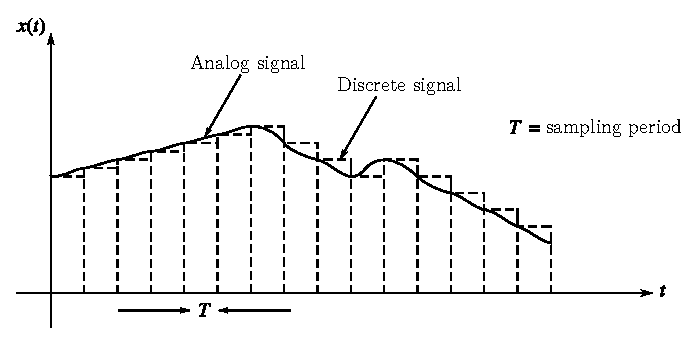
\includegraphics{chap5/fig5.1.eps}
\caption{Analog and discrete signal}\label{fig5.1}
\end{figure}

Then each sample of discrete signal is converted into a string of 0's and 1's (digitized) and the obtained signal is called digital signal. The digital signals could be processed with high speed with no disturbance from the noise. Digital signals could be processed independently at anytime other than the sampling period and is called off-line processing. If the signal is to be processed within the constraint of duration of time (eg: during sampling period), it is called on-line processing.

Digital signals (i.e., string of 0's and 1's) are processed using digital systems like digital computers, digital signal processors etc. using the concept of binary numbers and Boolean algebra (which refers ordinary algebra in some respects). The great advantage of digital signal is, it is less susceptible to disturbances (noise) compared to analog signal.

\section{Switching and Logic Levels}\label{sec5.2}

The digital systems are basically a discrete information (digital signal) processing systems. The signals may be in the form of voltage or current. The signals in all present day digital systems may have only two discrete values and are called binary. The binary may be either logic `0' or logic `1'. A logic value of 0 or 1 is often called a binary digit or bit. If an application requires more than two discrete levels, additional bits may be used. With `$n$' bits, we can have $2^{n}$ discrete levels or combinations.

Consider the two logic values of a binary signal shown in Fig.~\ref{fig5.2} below. One value must be higher than the other because the two values must be different in order to distinguish them.
\begin{figure}[H]
\centering
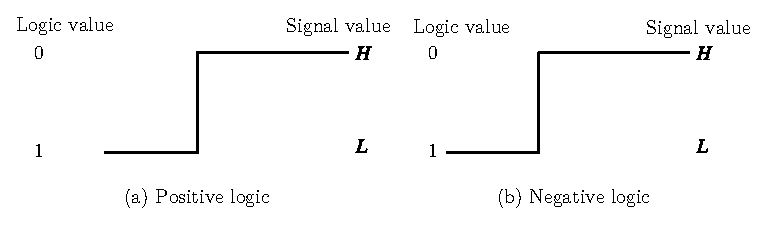
\includegraphics{chap5/fig5.2.eps}
\caption{Singal amplitude and logic assignment}\label{fig5.2}
\end{figure}

We designate the higher level of signal by $H$ and lower level by $L$. So there are 2 choices for the assignment of logic values. Choosing the higher level of signal $H$ as logic $L$ as in Fig.~\ref{fig5.2}(a) results in positive logic and choosing the lower level of signal $L$ as logic $l$ as in Fig.~\ref{fig5.2}(b) results in negative logic.
\begin{figure}[H]
\centering
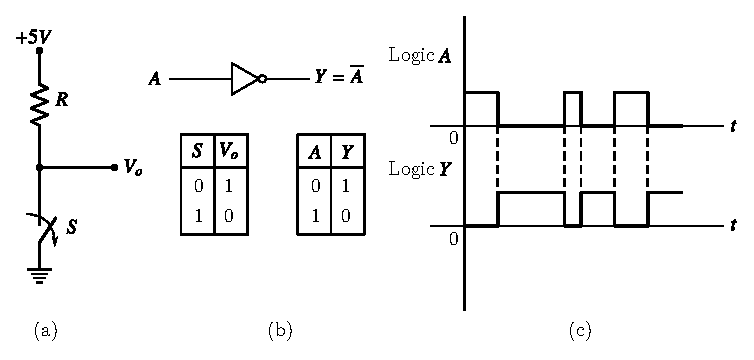
\includegraphics{chap5/fig5.3.eps}
\caption{(a) Switching circuit~ (b) Symbol \&\ truth table~ (c) Input/output waveform}\label{fig5.3}
\end{figure}

Consider a simple circuit shown in Fig.~\ref{fig5.3} below. The switch $S$ may be OFF or ON. The output voltage $\rmV_{\rmo}=5\rmV$ (HIGH). When $S$ is OFF and $\rmV_{\rmo}=0\rmV$ (LOW) when $S$ in ON. Assume that OFF as logic 0 and ON as logic 1 at the input and low as logic 0 and HIGH as logic 1 at the output, the circuit shown in Fig.~\ref{fig5.3} acts like an inverter i.e., the inpout 0 results in 1 at the output and vice versa. such circuits are known as logic gates and the particular gate under consideration is an inverter or NOT gate. The symbol and truth table of inverter or NOT gate is shown in Fig.~\ref{fig5.3}(b) below.


\smallskip
\itheading{Digital Waveform}

In electronic switching circuits, logic 0 and 1 are represented by voltage or current levels which are a range of values with clear margin between the high end of LOW and low end of HIGH. For eg. if logic 0 is ideally represented as 0V and logic 1 as 5V, the actual voltage ranges may be 0 to 0.2V and 3.7V to 5V with a forbidden region of 3.5V (i.e., $3.7-0.2=3.5\rmV$).

The digital waveforms for logic levels (ideal and actual) are shown in Fig.~\ref{fig5.4} below.
\begin{figure}[H]
\centering
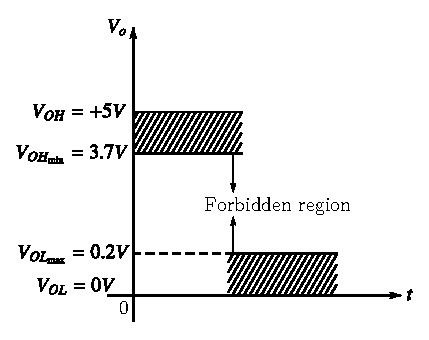
\includegraphics[scale=.95]{chap5/fig5.4.eps}
\caption{Logic level (ideal and actual)}\label{fig5.4}
\end{figure}
\vskip -.9cm
\begin{align*}
\text{Ideal~:}\quad & \text{Logic } 0=\rmV_{\rmo\rmL}=0\rmV\\[2pt]
                    & \text{Logic } 1=\rmV_{\rmo\rmH}=5\rmV\\[3pt]
\text{Actual~:}\quad & \rmV_{\rmo\rmL} <\text{ Logic } 0 <\rmV_{\rmo\rmL_{\max}}\\[2pt]
\therefore\quad & 0\leq \text{ logic } 0<0.2\rmV\\[2pt]
& \rmV_{\rmo\rmH_{\text{min}}}<\text{ Logic } 1< \rmV_{\rmo \rmH}\\[2pt]
\therefore\quad & 3.7\rmV < \text{ Logic } 1< 5\rmV
\end{align*}
$\therefore$~ Forbidden region = $(\rmV_{\rmo\rmH_{\min}}-\rmV_{\rmo\rmL_{\max}})=3.7-0.1=3.5\rmV$

In the forbidden region the signal cannot be recognized as either logic 0 or logic 1.

\vfill\eject

\smallskip
\itheading{Decimal Number System}

In regular day to day transactions, we use decimal number system in which only ten digits are used i.e., 0 to 9. Decimal number system is base 10 or radix 10 number system. The general form of a decimal number is,
$$
\rmd_{\rmm_{\rmc}}\rmd_{\rmm-1}\ldots \rmd_{3}\rmd_{2}\rmd_{1}\rmd_{0}\cdot \rmd_{-1}\rmd_{-2}\ldots \rmd_{-n}
$$
and its equivalent is given by,
\begin{align*}
\rmd_{\rmm}\times 10^{\rmm} &+ \rmd_{\rmm-1}\times 10^{\rmm-1}+\cdots+\rmd_{3}\times 10^{3}+\rmd_{2}\times 10^{2}+\rmd_{1}\times 10^{1}+\rmd_{0}\times 10^{0}\\
& + \rmd_{-1}\times 10^{-1}+d_{-2}\times 10^{-2}+\cdots+\rmd_{-n}\times 10^{-n}
\end{align*}

For example, consider a decimal number $(2504.187)_{10}$. The subscript or indicates the given number is in decimal or base 10 or radix 10 system. Its equivalents is given by,
\begin{align*}
&= 2\times 10^{3}+5\times 10^{2}+0\times 10^{1}+4\times 10^{0}+1\times 10^{-1}+8\times 10^{-2}+7\times 10^{-3}\\[3pt]
&= 2000+500+0+4+0.1+0.08+0.007\\[3pt]
&= (2504.187)_{\rmd}.
\end{align*}

In decimal number system instead of $\rmd$ we can use 10 also.

\smallskip
\itheading{Binary Number System}

In a digital electronic system, the active devices used are operated as switches and have only two states i.e., ON and OFF. For this reason, the binary numbering system is used in which only 2 digits i.e., 0 and 1 are allowed. So binary number system is base 2 or radix 2 number system.

The general form of a binary number is,
$$
\rmb_{\rmm}\rmb_{\rmm-1}\ldots \rmb_{3}\rmb_{2}\rmb_{1}\rmb_{0}\cdot \rmb_{-1}\rmb_{-2}\ldots \rmb_{-n}
$$
and decimal equivalent is given by,
\begin{align*}
\rmb_{\rmm}\times 2^{\rmm} &+ \rmb_{\rmm-1}\times 2^{\rmm-1}+\cdots+\rmb_{3}\times 2^{3}+\rmb_{2}\times 2^{2}+b_{1}\times 2^{1}+\rmb_{0}\times 2^{0}\\[3pt]
&+ \rmb_{-1}\times 2^{-1}+\rmb_{2}\times 2^{-2}+\cdots+\rmb_{-n}\times 2^{-n}
\end{align*}

For example, consider a binary number $=(1~1~0~1~1\,.\,1~1~0~1)_{2}$.

\eject

The subscript 2 or $\rmb$ indicates that the given number is in binary or base 2 or radix 2 system. Its decimal equivalent is,
\begin{align*}
&= 1\times 2^{4}+14\times 2^{3}+04\times 2^{2}+1\times 2^{1}+1\times 2^{0}\\
&\quad +1\times 2^{-1}+1\times 2^{-2}+0\times 2^{-3}+1\times 2^{-4}\\
&=16+8+0+2+1+0.5+0.25+0+0.0625\\
&=(27.8125)_{10}
\end{align*}

The subscript 10 indicates that the number is in decimal or base 10 or radix 10 system.

In a binary number, each digit is called bit.

The left most bit of a binary number is called most significant bit (MSB) and right most bit is called least significant bit (LSB).

\smallskip
\itheading{Octal and Hexadecimal Numbers}

Decimal (base 10 or radix 10) number system is must because, we use it in day-to-day transactions and binary (base 2 or radix 2) is important because binary numbers can be processed directly by digital system. Number in other radices or bases are not often processed directly, but they may be important for documentation or other purposes.

In particular, the radix 8 and radix 16 provide simple shorthand representations of multibit numbers in a digital system. The radix-8 system is also called an octal system and radix-16 system is also called hexadecimal system. The octal system needs 8 digits (0 to 9 and A to F. A to F are used to represent 10 to 15 respectively).

The general form of are octal number is,
$$
\rmO_{\rmm}\rmO_{\rmm-1}\ldots \rmO_{3}\rmO_{2}\rmO_{1}\rmO_{0}\cdot \rmO_{-1}\rmO_{-2}\ldots \rmO_{-n}
$$
and its decimal equivalent is given by,
\begin{align*}
\rmO_{\rmm}\times 8^{\rmm} &+ \rmO_{\rmm-1}\times 8^{\rmm-1}+\cdots+\rmO_{3}\times 8^{3}+\rmO_{2}\times 8^{2}+\rmO_{1}\times 8^{1}+\rmO_{0}\times 8^{0}\\
&+ \rmO_{-1}\times 8^{-1}+\rmO_{-2}\times 8^{-2}+\cdots+\rmO_{-\rmn}\times 8^{-\rmn}
\end{align*}

For example consider a number $=(736.52)_{0}$. The subscript `8' or `O' indicates that the given number is in octal system. Its decimal equivalent is given by,
\begin{align*}
&= 7\times 8^{2}+3\times 8^{1}+6\times 8^{0}+5\times 8^{-1}+2\times 8^{-2}\\
&= 448+24+6+0.625+0.03125\\
&= (478.65625)_{10}.
\end{align*}

Similarly, the general form of a hexadecimal number is given by,
$$
\rmH_{\rmm}\rmH_{\rmm-1}\ldots \rmH_{3}\rmH_{2}\rmH_{1}\rmH_{0}\cdot \rmH_{-1}\rmH_{-2}\ldots \rmH_{-\rmn}
$$
and its decimal equivalent is given by,
\begin{align*}
\rmH_{\rmm}\times 16^{\rmm} &+ \rmH_{\rmm-1}\times 16^{\rmm-1}+\cdots+\rmH_{3}\times 16^{3}+\rmH_{2}\times 16^{2}+\rmH_{1}\times 16^{1}+\rmH_{0}\times 16^{0}\\
&+ \rmH_{-1}\times 16^{-1}+\rmH_{-2}\times 16^{-2}+\cdots \rmH_{-\rmn}\times 16^{\rmn}.
\end{align*}

For example, consider a hexadecimal number (A3F2.5E)$_{16}$ = (A3F2.5E)$_{\rmH}$. The subscript 16 or H indicates that the given number is in hexadecimal system. Its decimal equivalent is given by,
\begin{align*}
&= 10\times 16^{3}+3\times 16^{2}+15\times 16^{1}+2\times 16^{0}+5\times 16^{-1}+14\times 16^{-2}\\
&= (41970.367875)_{10}.
\end{align*}

\begin{center}
\rule{4cm}{1pt}\\
{\bf\Large Problems}\\[-3pt]
\rule{4cm}{1pt}
\end{center}

\begin{problem}\label{prob5.1}
Convert the following binary numbers into decimal system.

\medskip
\noindent
(i)~ (1 0 1 1)$_{2}$\hfil~~ (ii)~ (1 1 1 0 1\,.\,0 1)$_{2}$\hfil~~
(iii)~  (1 1 1 1 1 0 1 0 1)$_{2}$\hfil~~ (iv)~ (1 0 1 0 1 0\,.\,1 0 1)$_{2}$
\end{problem}

\begin{solution}
\begin{itemize}
\item[(i)] (1 0 1 1)$_{2}$

\qquad~~~~~~~~ = $1\times 2^{3}+0\times 2^{2}+1\times 2^{1}+1\times 2^{0}$

\qquad~~~~~~~~ = (1 1)$_{10}$

\item[(ii)]
\begin{tabbing}
\= (1 1 1 0 1\,.\,0 1)$_{2}$\\[3pt]
\> = $1\times 2^{4}+1\times 2^{3}+1\times 2^{2}+0\times 2^{1}+1\times 2^{0}+0\times 2^{-1}+1\times 2^{-2}$\\[3pt]
\> = $(29.25)_{10}$
\end{tabbing}

\item[(iii)]
\begin{tabbing}
\= (1 1 1 1 1 0 1 0 1)$_{2}$\\[3pt]
\>= $1\times 2^{8}+1\times 2^{7}+1\times 2^{6}+1\times 2^{5}+1\times 2^{4}+0\times 2^{3}+$\\[3pt]
\>~ $1\times 2^{2}+0\times 2^{1}+1\times 2^{0}$\\[3pt]
\>= $(501)_{10}$
\end{tabbing}

\item[(iv)]
\begin{tabbing}
\= (1 0 1 0 1 0\,.\,1 0 1)$_{2}$\\[4pt]
\>= $1\times 2^{5}+0\times 2^{4}+1\times 2^{3}+0\times 2^{2}+1\times 2^{1}+0\times 2^{0}+$\\[4pt]
\>~ $1\times 2^{-1}+0\times 2^{-2}+1\times 2^{-3}$\\[4pt]
\>= $(42.625)_{10}$
\end{tabbing}
\end{itemize}
\end{solution}

\begin{problem}\label{prob5.2}
Convert the following octal numbers into decimal system.

\medskip
(i)~ $(7034)_{8}$\hfil (ii)~ $(624.36)_{8}$\hfil
(iii) $(1616.16)_{8}$\hfil (iv)~  (1 0 1 0 1 0)$_{8}$
\end{problem}

\begin{solution}
\begin{itemize}
\item[(i)] $(7034)_{8}$

\qquad~~~~~~~~ = $7\times 8^{3}+0\times 8^{2}+3\times 8^{1}+4\times 8^{0}$

\qquad~~~~~~~~ = $(3612)_{10}$

\item[(ii)] 
\begin{tabbing}
\=$(624.36)_{8}$\\[4pt]
\>= $6\times 8^{2}+2\times 8^{1}+4\times 8^{0}+3\times 8^{-1}+6\times 8^{-2}$\\[4pt]
\>= $(404.46875)_{10}$
\end{tabbing}

\item[(iii)]
\begin{tabbing}
\=$(1616.16)_{8}$\\[4pt]
\>= $1\times 8^{3}+6\times 8^{2}+1\times 8^{1}+6\times 8^{0}+1\times 8^{-1}+6\times 8^{-2}$\\[4pt]
\>= $(910.21875)_{10}$
\end{tabbing}

\item[(iv)]
\begin{tabbing}
\=(1 0 1 0 1 0)$_{8}$\\[4pt]
\>= $1\times 8^{5}+0\times 8^{4}+1\times 8^{3}+0\times 8^{2}+1\times 8^{1}+0\times 8^{0}$\\[4pt]
\>= $(33288)_{10}$
\end{tabbing}
\end{itemize}
\end{solution}

\begin{problem}\label{prob5.3}
Convert the following hexadecimal numbers into decimal system.

\medskip
(i)~ (A38)$_{16}$\hfil (ii)~  (834.41)$_{16}$\hfil
(iii)~ (ABC.D)$_{16}$\hfil (iv)~ (1 1 1 0\,.\,0 1)$_{16}$
\end{problem}

\eject

\begin{solution}
\begin{itemize}
\item[(i)] (A38)$_{16}$

\qquad~~~ = $10\times 16^{2}+3\times 16^{1}+8\times 16^{0}$

\qquad~~~ = $(2616)_{10}$

\item[(ii)]
\begin{tabbing}
\== $(834.41)_{10}$\\[4pt]
\>= $8\times 16^{2}+3\times 16^{1}+4\times 16^{0}+4\times 16^{-1}+1\times 16^{-2}$\\[4pt]
\>= $(2100.25390625)_{10}$
\end{tabbing}

\item[(iii)] 
\begin{tabbing}
\==(ABC.D)$_{16}$\\[4pt]
\>= $10\times 16^{2}+11\times 16^{1}+12\times 16^{0}+13\times 16^{-1}$\\[4pt]
\>= $(2748.8125)_{10}$
\end{tabbing}

\item[(iv)] 
\begin{tabbing}
\=(1 1 1 0\,.\,0 1)$_{16}$\\[4pt]
\>= $1\times 16^{3}+1\times 16^{2}+1\times 16^{1}+0\times 16^{0}+0\times 16^{-1}+1\times 16^{-2}$\\[4pt]
\>= $(4368.00390625)_{10}$
\end{tabbing}
\end{itemize}
\end{solution}

\section{Number Base Conversion}\label{sec5.3}

In this section, we will discuss to convert a given number from one base to another.

\smallskip
\heading{(i) Decimal to any base-r}

Consider a given decimal number has both integer and fractional parts. The integer part of the decimal number is converted to base-r integer number, by successive division by r and the fractional part is converted to base-r fractional number by successive multiplication by r. The integer part of the decimal number is to be successively divided by r, till the quotient becomes zero. The last remainder is the MSB. The remainders read from bottom to top, give the equivalent base-r integer number. The fractional part of the decimal number is to be successively multiplied by r, till the fractional part of the product comes to zero or till the desired accuracy is obtained. The first integer obtained is MSB. Thus the integers read from top to bottom, give the base-r fractional number.

For example, consider a decimal number $(398.75)_{10}$. Say we want to convert it into binary. (i.e. base-r = 2). The integer part is 398 and fractional part is 75.

To convert the integer part into binary, divide 398 by 2 successively, till the quotient becomes zero and collect the remainders from bottom to top as below.
\begin{figure}[H]
\centering
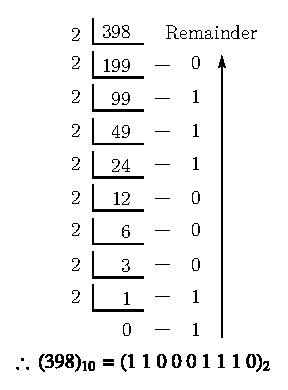
\includegraphics[scale=.9]{chap5/div1.eps}
\end{figure}


To convert the fractional part into binary, multiply 75 by 2 successively, till the fractional part of the product becomes zero or till the desired accuracy is obtained as below.
\begin{figure}[H]
\centering

\includegraphics{chap5/div2.eps}
\end{figure}

Combining we get,
$$
(398.75)_{10}=(1~1~0~0~0~1~1~1~0\,.\,1~1)_{2}
$$

\begin{center}
\rule{4cm}{1pt}\\
{\bf\Large Problems}\\[-3pt]
\rule{4cm}{1pt}
\end{center}

\begin{problem}\label{prob5.4}
Convert $(734)_{10}$ into binary.
\end{problem}

\begin{solution}
~
\begin{figure}[H]
\centering
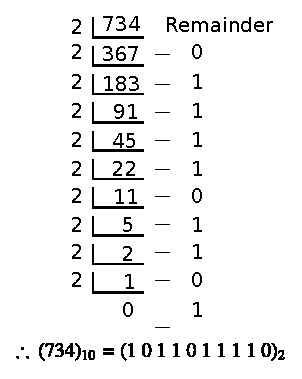
\includegraphics[scale=.9]{chap5/div3.eps}
\end{figure}
\end{solution}

\begin{problem}\label{prob5.5}
Perform the following $(2003)_{10}=(?)_{2}$.
\end{problem}

\begin{solution}
~
\begin{figure}[H]
\centering
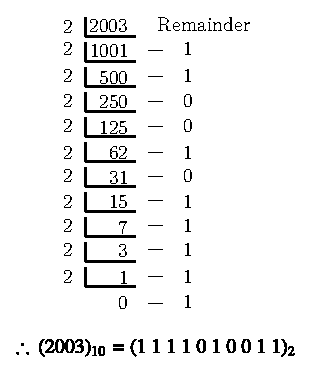
\includegraphics[scale=1.05]{chap5/div4.eps}
\end{figure}
\end{solution}

\begin{problem}
Convert $(1593.875)_{10}$ into binary.
\end{problem}

\begin{solution}
~
\begin{figure}[H]
\centering
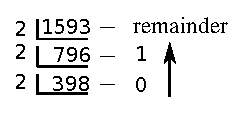
\includegraphics{chap5/div5a.eps}
\end{figure}
\begin{figure}[H]
\centering
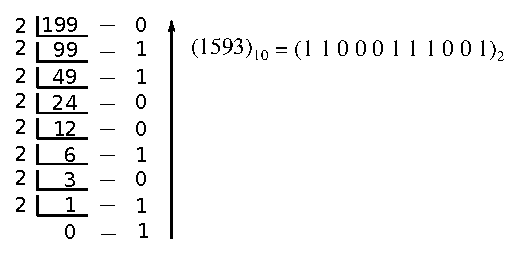
\includegraphics{chap5/div5.eps}
\end{figure}
\begin{figure}[H]
\centering
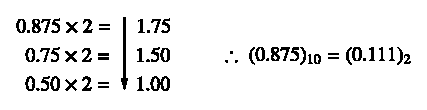
\includegraphics{chap5/div6.eps}
\end{figure}
$$
\therefore\quad (1593.875)_{10}=(1~1~0~0~0~1~1~1~0~0~1\,.\,1~1~1)_{2}
$$
\end{solution}

\begin{problem}\label{prob5.7}
Convert $(0.705)_{10}$ into binary.
\end{problem}

\begin{solution}
~
\begin{figure}[H]
\centering
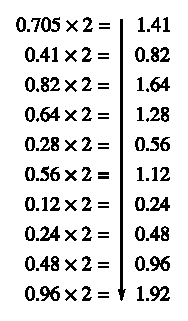
\includegraphics{chap5/div7.eps}
\end{figure}

This number cannot be represented accurately in binary.
$$
\therefore\quad (0.705)_{10}=(0\,.\,1~0~1~1~0~1~0~0~0~1\ldots)_{2}.
$$
\end{solution}

\begin{problem}\label{prob5.8}
Convert $(1~0~1~0\,.\,1~0~1)_{10}$ into binary.
\end{problem}

\begin{solution}
~
\begin{figure}[H]
\centering
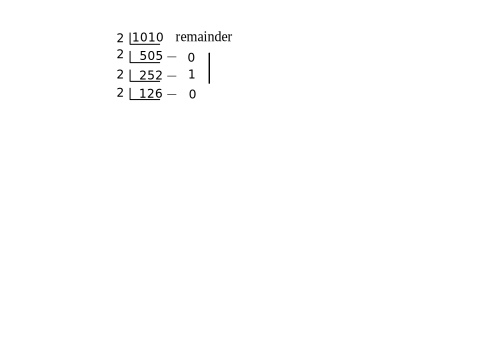
\includegraphics{chap5/div8.eps}
\end{figure}
\begin{figure}[H]
\centering
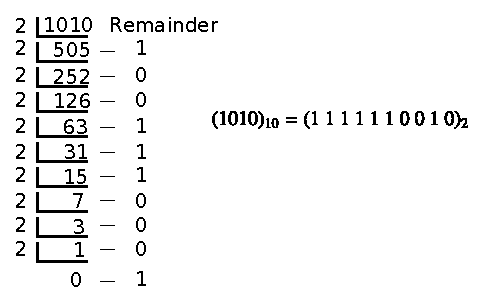
\includegraphics{chap5/div9.eps}
\end{figure}
\begin{figure}[H]
\centering
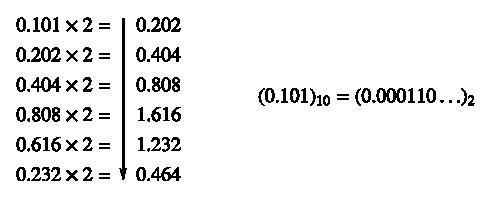
\includegraphics[scale=.97]{chap5/div9a.eps}
\end{figure}
$$
\therefore\quad (1~0~1~0\,.\,1~0~1)_{10}=(1~1~1~1~1~1~0~0~1~0\,.\,0~0~0~1~1~0...)_{2}
$$
\end{solution}

\begin{problem}\label{prob5.9}
Convert $(934)_{10}$ into octal.
\end{problem}

\begin{solution}
~
\begin{figure}[H]
\centering
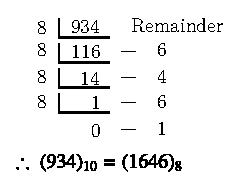
\includegraphics{chap5/div10.eps}
\end{figure}
\end{solution}

\begin{problem}\label{prob5.10}
Perform the following $(2003)_{10}=(?)_{8}$.
\end{problem}

\begin{solution}
~
\begin{figure}[H]
\centering
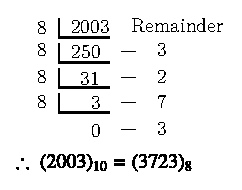
\includegraphics{chap5/div11.eps}
\end{figure}
\end{solution}

\begin{problem}\label{prob5.11}
Convert $(11582.875)_{10}$ into octal.
\end{problem}

\begin{solution}
~
\begin{figure}[H]
\centering
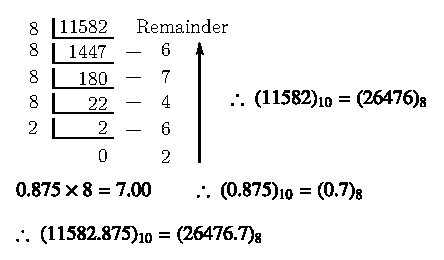
\includegraphics{chap5/div12.eps}
\end{figure}
\end{solution}

\vfill\eject

\begin{problem}\label{prob5.12}
Convert $(0.705)_{10}$ into octal.
\end{problem}

\begin{solution}
~
\begin{figure}[H]
\centering
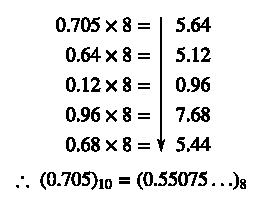
\includegraphics[scale=1.07]{chap5/div13.eps}
\end{figure}
\end{solution}

\begin{problem}\label{prob5.13}
Convert $(8899)_{10}$ into hexadecimal.
\end{problem}

\begin{solution}
~
\begin{figure}[H]
\centering
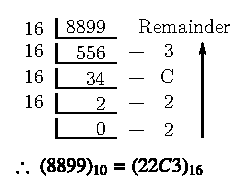
\includegraphics[scale=1.07]{chap5/div14.eps}
\end{figure}
\end{solution}

\begin{problem}\label{prob5.14}
Perform the following~:
$$
(894867)_{10}=(?)_{16}
$$
\end{problem}

\begin{solution}
~
\begin{figure}[H]
\centering
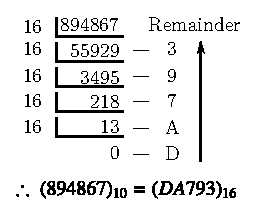
\includegraphics[scale=1.07]{chap5/div15.eps}
\end{figure}
\end{solution}

\eject

\begin{problem}\label{prob5.15}
Convert $(7084.95)_{10}$ into hexadecimal.
\end{problem}

\begin{solution}
~
\begin{figure}[H]
\centering
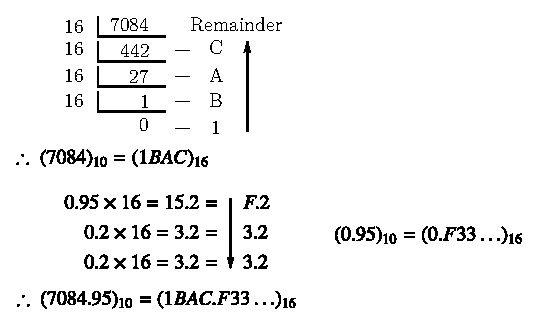
\includegraphics{chap5/div16.eps}
\end{figure}
\end{solution}

\begin{problem}\label{prob5.16}
Convert $(0.368)_{10}$ into hexadecimal.
\end{problem}

\begin{solution}
~
\begin{figure}[H]
\centering
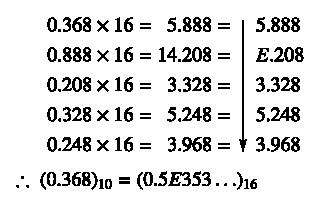
\includegraphics{chap5/div17.eps}
\end{figure}
\end{solution}

\begin{problem}\label{prob5.17}
Convert $(4477.85)_{10}$ into hexadecimal.
\end{problem}

\begin{solution}
~
\begin{figure}[H]
\centering
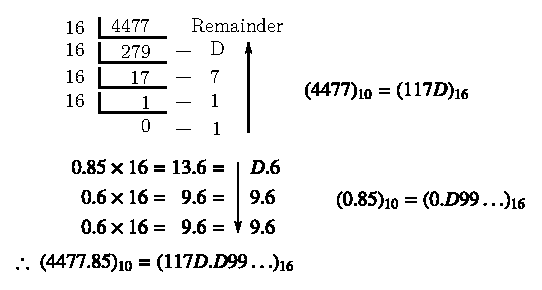
\includegraphics{chap5/div18.eps}
\end{figure}
\end{solution}

\smallskip
\heading{(ii) Binary to octal~:}

We know that in octal system, we use 8 digits i.e., 0 to 7. Since a string of 3 bits can take on 8 different combinations, it follows that each 3 bit string can be uniquely represented by one octal digit as shown in Table~\ref{tab7.1}.
\begin{table}[H]
\centering
\caption{}\label{tab7.1}
\renewcommand{\arraystretch}{1.2}
\tabcolsep=15pt
\begin{tabular}{|c|c|}
\hline
{\bf Octal} & {\bf Binary}\\[3pt]
\hline
0 & 000\\
1 & 001\\
2 & 010\\
3 & 011\\
4 & 100\\
5 & 101\\
6 & 110\\
7 & 111\\
\hline
\end{tabular}
\end{table}

Thus, it is very easy to convert a binary number to an octal. Starting at the binary point, we simply separate the bits into groups of three and replace each group with the corresponding octal digit.
\begin{align*}
\text{For example~: Consider~} & (\underbrace{110}_{6} \ \ \underbrace{101}_{5} \ \ \underbrace{111}_{7} \ \ \underbrace{011}_{3} \ \ \underbrace{101}_{5} \ \ \underbrace{101}_{5} \ \ \underbrace{110}_{6})_{2}\\[4pt]
&= (65735.56)_{8}
\end{align*}

In this procedure, we can freely add zeroes on the left of integer part and on the right of fractional part to make the total number of bits, multiples of 3 as required.

\medskip
\heading{(iii)~ Octal to binary~:}

Converting from octal to binary is also very easy. We simply replace each octal digit with the corresponding 3 bit string.
\begin{align*}
\text{For example~:~} & \text{Consider~ } (7~4~6~3~.~2~4~5)_{8}\\[3pt]
                      & \overbrace{111}^{7} \ \ \overbrace{100}^{4} \ \ \overbrace{110}^{6} \ \ \overbrace{011}^{3} \ \ \overbrace{010}^{2} \ \ \overbrace{100}^{4} \ \ \overbrace{101}^{5}\\[3pt]
\therefore\quad (7463.245)_{8} &= (1~1~1~1~0~0~1~1~0~0~1~1\,.\,0~1~0~1~0~0~1~0~1)_{2}
\end{align*}

\begin{center}
\rule{4cm}{1pt}\\
{\bf\Large Problems}\\[-3pt]
\rule{4cm}{1pt}
\end{center}

\begin{problem}\label{prob5.18}
Convert $(1~1~0~1~1~1~1~0~1~0\,.\,0~1~1~1~0~1~1)_{2}$ into octal.
\end{problem}

\begin{solution}
$\underbrace{011}_{3} \ \ \underbrace{011}_{3} \ \ \underbrace{111}_{7} \ \ \underbrace{010}_{2} \ \ \underbrace{011}_{3} \ \ \underbrace{101}_{5} \ \ \underbrace{100}_{4}$
$$
\therefore\quad (1~1~0~1~1~1~1~1~0~1~0\,.\,0~1~1~0~1~1)_{2}=(3372.354)_{8}
$$
\end{solution}

\begin{problem}\label{prob5.19}
Convert the following into octal.
\begin{itemize}
\item[(i)] $(1~1~0~1~1~0~1~1~1~1~0)_{2}$

\item[(ii)] $(1~1~1~0~1~1~0~1~1~1~0\,.\,1~1~1~0~1)_{2}$

\item[(iii)] $(0\,.\,1~1~1~1~0~1~0~1~1~0~1)_{2}$
\end{itemize}
\end{problem}

\begin{solution}
\begin{itemize}
\item[(i)] $\underbrace{011}_{3} \ \ \underbrace{011}_{3} \ \ \underbrace{011}_{3} \ \ \underbrace{110}_{6}$

\smallskip
\qquad\quad~~~ $\therefore~ (1~1~0~1~1~0~1~1~1~1~0)_{2}=(3336)_{8}$

\item[(ii)] $\underbrace{011}_{3} \ \ \underbrace{101}_{5} \ \ \underbrace{101}_{5} \ \ \underbrace{110}_{6} \ \ \underbrace{111}_{7} \ \ \underbrace{010}_{2}$

\smallskip
$\therefore~ (1~1~1~0~1~1~0~1~1~1~0\,.\,1~1~1~0~1)_{2}=(3556.72)_{8}$

\item[(iii)] $0 \ \ \underbrace{111}_{7} \ \ \underbrace{101}_{5} \ \ \underbrace{011}_{3} \ \ \underbrace{010}_{2}$

\smallskip
$\therefore$~ $(0\,.\,1~1~1~1~0~1~0~1~1~0~1)_{2}=(0.7532)_{8}$
\end{itemize}
\end{solution}

\heading{(iv)~ Binary to hexadecimal~:}

In hexadecimal system, we use 16 digits. i.e., 0 to 7 and A to F. Since a string of 4 bits can take on 16 different combinations, it follows that each 4 bit string can be uniquely represented by one hexadecimal digit as shown in Table~\ref{tab5.2}.
\begin{table}[H]
\centering
\caption{}\label{tab5.2}
\renewcommand{\arraystretch}{1.2}
\tabcolsep=10pt
\begin{tabular}{|c|c|c|c|}
\hline
{\bf Hexadecimal} & {\bf Binary} & {\bf Hexadecimal} & {\bf Binary}\\[3pt]
\hline
0 & 0 0 0 0 & 8 & 1 0 0 0\\
1 & 0 0 0 1 & 9 & 1 0 0 1\\
2 & 0 0 1 0 & A & 1 0 1 0\\
3 & 0 0 1 1 & B & 1 0 1 1\\
4 & 0 1 0 0 & C & 1 1 0 0\\
5 & 0 1 0 1 & D & 1 1 0 1\\
6 & 0 1 1 0 & E & 1 1 1 0\\
7 & 0 1 1 1 & F & 1 1 1 1\\
\hline
\end{tabular}
\end{table}

Thus, it is very easy to convert a binary number to hexadecimal. Starting at the binary point, we simply separate the bits into groups of 4 and replace each group with the corresponding hexadecimal digit.
\begin{align*}
\text{For example~: Consider~ } & (\underbrace{1~0~1~1}_{\rmB} \ \ \underbrace{0~1~1~1}_{7} \ \ \underbrace{1~0~1~1}_{\rmB} \ \ \underbrace{1~1~1~0}_{\rmE} \ \ \underbrace{1~1~1~0}_{\rmE} \ \ \underbrace{0~0~1~1}_{3})_{2}\\[3pt]
&= \text{(B7BE.E3)}_{16} 
\end{align*}

In this procedure also, we can freely add zeroes on the left of integer part and on the right of fractional part to make the total number of bits, multiples of 4 as required.

\smallskip
\heading{(v)~ Hexadecimal to binary~:}

Converting from hexadecimal to binary is also very easy. We simply replace each hexadecimal digit with the corresponding 4 bit string.
\begin{align*}
\text{For example~:~} &(\text{8BE6.7A})_{16}\\[3pt]
& \overbrace{1~0~0~0}^{8} \ \ \overbrace{1~0~1~1}^{\rmB} \ \ \overbrace{1~1~1~0}^{\rmE} \ \ \overbrace{0~1~1~0}^{6} \ \ \overbrace{0~1~1~1}^{7} \ \ \overbrace{1~0~1~0}^{\rmA}\\[3pt]
\therefore\quad (\text{8BE6.7A})_{16} &= (1~0~0~0 \ \ \ 1~0~1~1 \ \ \ 1~1~1~0 \ \ \ 0~1~1~0\,.\,0~1~1~1 \ \ \ 1~0~1~0)_{2}
\end{align*}

\eject

\begin{center}
\rule{4cm}{1pt}\\
{\bf\Large Problems}\\[-3pt]
\rule{4cm}{1pt}
\end{center}

\begin{problem}\label{prob5.20}
Convert (1 1 0 1 1 1 1 1 0 1 1 0 1 1\,.\,0 1 1 0 1)$_{2}$ into hexadecimal.
\end{problem}

\begin{solution}
$\underbrace{0~0~1~1}_{3} \ \ \underbrace{0~1~1~1}_{7} \ \ \underbrace{1~1~0~1}_{\rmD} \ \ \underbrace{1~0~1~1}_{\rmB} \ \ \underbrace{0~1~1~0}_{6} \ \ \underbrace{1~0~0~0}_{8}$
$$
\therefore\quad (1~1~0~1~1~1~1~1~0~1~1~0~1~1\,.\,0~1~1~0~1)_{2}=(\text{37DB.68})_{16}
$$
\end{solution}

\begin{problem}\label{prob5.21}
Convert the following into hexadecimal.
\begin{itemize}
\item[(i)] (1 1 0 1 1 1 1 0 1\,.\,0 1)$_{2}$

\item[(ii)] (1 1 0 1 1 1 1 0 1 0 1 1 1 0 1)$_{2}$

\item[(iii)] (0\,.\,1 1 0 1 0 1 0 1 1 1 0 1 1)$_{2}$
\end{itemize}
\end{problem}

\begin{solution}
\begin{itemize}
\item[(i)] $\underbrace{0~0~0~1}_{1} \ \ \underbrace{1~0~1~1}_{\rmB} \ \ \underbrace{1~1~0~1}_{\rmD} \ \ \underbrace{0~1~0~0}_{4}$

\smallskip
\qquad\quad~~~ $\therefore$~ (1 1 0 1 1 1 1 0 1\,.\,0 1)$_{2}$ = (1BD.4)$_{16}$

\item[(ii)] $\underbrace{0~1~1~0}_{6} \ \ \underbrace{1~1~1~1}_{\rmF} \ \ \underbrace{0~1~0~1}_{5} \ \ \underbrace{1~1~0~1}_{\rmD}$

\smallskip
$\therefore$~ (1 1 0 1 1 1 1 0 1 0 1 1 1 0 1)$_{2}$ = (6F5D)$_{16}$

\item[(iii)] $0 \ \ \underbrace{1~1~0~1}_{\rmD} \ \ \underbrace{0~1~0~1}_{5} \ \ \underbrace{1~1~0~1}_{\rmD} \ \ \underbrace{1~0~0~0}_{8}$

\smallskip
$\therefore$~ (0\,.\,1 1 0 1 0 1 0 1 1 1 0 1 1)$_{2}$ = (0.D5D8)$_{16}$
\end{itemize}
\end{solution}

\begin{problem}\label{prob5.22}
Find the binary, octal and hexadecimal equivalent of the following decimal numbers.
\begin{itemize}
\item[(i)] (345.75)$_{10}$

\item[(ii)] (44355)$_{10}$

\item[(iii)] (0.7585)$_{10}$
\end{itemize}
\end{problem}

\begin{solution}
\begin{itemize}
\item[(i)] (345.75)$_{10}$
\begin{figure}[H]
\centering
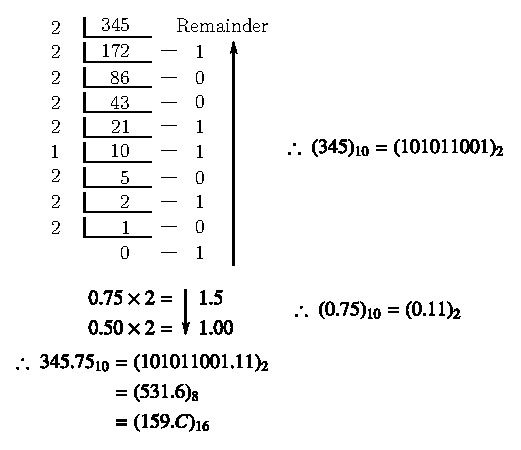
\includegraphics{chap5/div19.eps}
\end{figure}

\item[(ii)] (44355)$_{10}$
\begin{figure}[H]
\centering
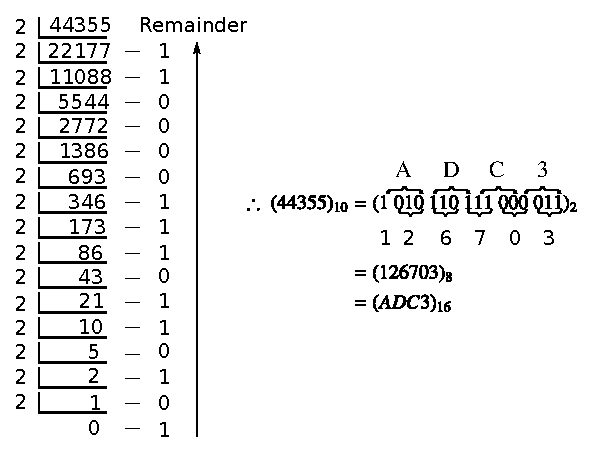
\includegraphics{chap5/div20.eps}
\end{figure}

\eject

\item[(iii)] $(0.7585)_{10}$
\begin{figure}[H]
\centering
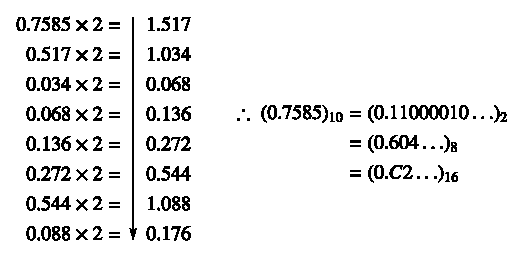
\includegraphics{chap5/div21.eps}
\end{figure}
\end{itemize}
\end{solution}

\section{Complements}\label{sec5.4}

For a given number N in base-r, we can define two types of complements.
\begin{itemize}
\item[(i)] r's complement

\item[(ii)] (r$-$1)'s complement
\end{itemize}

With the concept of complements, the subtraction operations and logical manipulations become easy in digital computers.

Consider a given positive number N in base-r with an integer part of n digits and a fractional part of m digits. Then the r's complement is given by,
\begin{alignat*}{2}
&= (\rmr^{\rma}-\rmN) &\qquad& ;\text{ for~ } \rmN\neq 0\\
&= 0                 &\qquad& ; \text{ for~ } \rmN = 0
\end{alignat*}
and the (r$-$1)'s complement is given by,
$$
=(\rmr^{\rmn}-\rmr^{-\rmm}-\rmN)
$$

For example, consider a decimal number (5734.35)$_{10}$. Here base r = 10. So we can define 10's complement (r's complement) and 9's complement ((r$-1$1)'s complement) for this number. In (5734.35)$_{10}$, number of digits in integer part is n = 4 and that in fractional part is m = 2.
\begin{align*}
\therefore\quad \text{10's complement of } (5734.35)_{10} &= 10^{4}-5734.35\\[3pt]
 &= (10000-5734.35)_{10}\\[3pt]
 &= 4265.65\\[3pt]
\text{and 9's complement of } (5734.35)_{10} &= 10^{4}-10^{-2}-5734.35\\[3pt]
&= (9999.99-5734.35)_{10}\\[3pt]
&= 4265.64
\end{align*}

Note that 10's complement of a decimal number can be obtained by leaving all least significant zeros unchanged, subtracting the first non-zero least significant digit from 10 and then subtracting all other higher significant digits from 9. The 9's complement of a decimal number is obtained simply by subtracting every digit from 9.

As another example, consider a binary number (1 0 1 1 0 0\,.\,0 1 1 0)$_{2}$. Here base r = 2. So we can define 2's complement and 1's complement for this number. In (1 0 1 1 0 0\,.\,0 1 1 0)$_{2}$, the number of digits in integer part is n = 6 and that in fractional part is m = 4.
\begin{align*}
\therefore~ \text{2's complement of } (1~0~1~1~0~0\,.\,0~1~1~0)_{2} &= (2^{6})_{10}-(1~0~1~1~0~0\,.\,0~1~1~0)_{2}\\[3pt]
&= (1~0~0~0~0~0~0 - 1~0~1~1~0~0\,.\,0~1~1~0)_{2}\\[3pt]
&= (0~1~0~0~1~1\,.\,1~0~1~0)\\[3pt]
\text{and 1's complement of (1 0 1 1 0 0\,.\,0 1 1 0)} &=(2^{6}-2^{-4})_{10}-(1~0~1~1~0~0\,.\,0~1~1~0)_{2}\\[3pt]
&= 0~1~0~0~1~1\,.\,1~0~0~1
\end{align*}

Note that the 2's complement of a binary number can be obtained by leaving all least significant zeros, the first least significant 1 unchanged and then replacing 1's by 0s and 0's by 1's.

The 1's complement of a binary number can be obtained easily by replacing 1's by 0's and 0's by 1's.
\begin{note}
If we take complement of complement of a number, the number turns to its original value.
\end{note}
\begin{center}
\rule{4cm}{1pt}\\
{\bf\Large Problems}\\[-3pt]
\rule{4cm}{1pt}
\end{center}

\begin{problem}\label{prob5.23}
Find the 10's and 9's complement of the following decimal numbers.
\begin{center}
\begin{tabular}{r@{\;}l@{\qquad}r@{\;}l@{\qquad}r@{\;}l}
(i) & 13579 & (ii) & 900900 & (iii) &  00000\\[4pt]
(iv) & 8374.59 & (v) & 17850.6584 & (vi) & 0.1035
\end{tabular}
\end{center}
\end{problem}

\eject

\begin{solution}
Given numbers are in decimal i.e., base r = 10.
\begin{itemize}
\item[(i)] $(13579)_{10}$\qquad ;~ Here n = 5 and m = 0
\begin{align*}
\therefore\quad \text{10's complement of } (13579)_{10} &= 10^{5}-13579\\[3pt]
&= 100000-13579\\[3pt]
&= 86421\\[3pt]
\text{and 9's complement of } (13579)_{10} &= 10^{5}-10^{-0}-13579\\[3pt]
&= 99999-13579\\[3pt]
&= 86420
\end{align*}

\item[(ii)] $(900900)_{10}$\qquad ;~ Here n = 6 and m = 0
\begin{align*}
\therefore~ \text{10's complement of } (900900)_{10} &= 10^{6}-900900\\[3pt]
&= 1000000 - 900900\\[3pt]
&= 099100\\[3pt]
\text{and 9's complement of } (900900)_{10} &= 10^{6}-10^{-0}-900900\\[3pt]
 &= 999999-900900\\[3pt]
 &= 099099
\end{align*}

\item[(iii)] $(00000)_{10}$\qquad ; Here n = 5 and m = 0.

The 10's complement of zero is zero. See the definition in Sec.~\ref{sec5.4}.
\begin{align*}
\therefore~ \text{9's complement of } (00000)_{10} &= 10^{5}-10^{-0}-00000\\[3pt]
                                                  &= 99999
\end{align*}

\item[(iv)] $(8374.59)_{10}$\qquad ; Here n = 4 and m = 2
\begin{align*}
\therefore~ \text{10's complement of } (8374.59)_{10} &= 10^{4}-8374.59\\[3pt]
&= 1625.41\\[3pt]
\text{and 9's complement of } (8374.59)_{10} &= 10^{4}-10^{-2}-8374.59\\[3pt]
&= 1625.40
\end{align*}

\item[(v)] $(17850.6584)_{10}$\qquad ; Here n = 5 and m = 4
\begin{align*}
\therefore~ \text{10's complement of } (17850.6584)_{10} &= 10^{5}-17850.6584\\[1pt]
&= 82149.3416\\[1pt]
\text{and 9's complement of } (17850.6584)_{10} &= 10^{5}-10^{-4}-17850.6584\\[1pt]
&= 82149.3415
\end{align*}

\item[(vi)] $(0.1035)_{10}$\qquad ; Here n = 0 and m = 4
\begin{align*}
\therefore~ \text{10's complement of } (0.1035)_{10} &= 10^{0}-0.1035\\[1pt]
&= 0.8965\\[1pt]
\text{and 9's complement of } (0.1035)_{10} &= 10^{0}-10^{-4}-0.1035\\[1pt]
&= 0.8964
\end{align*}
\end{itemize}
\end{solution}

\begin{problem}\label{prob5.24}
Find the 2's and 1's complement of the following binary numbers.
\begin{itemize}
\item[(i)] (1 0 1 0 1 1)$_{2}$\qquad\quad (ii)~ (1 1 1 1 1 0 1 0)$_{2}$
\end{itemize}
\end{problem}

\begin{solution}
Given numbers are in binary i.e., r = 2
\begin{itemize}
\item[(i)] $(1~0~1~0~1~1)_{2}$\qquad ; Here n = 6 and m = 0
\begin{align*}
\therefore~ \text{2's complement of } (1~0~1~0~1~1)_{2} &= (2^{6})_{10}-(1~0~1~0~1~1)_{2}\\[1pt]
&= (1~0~0~0~0~0~0-1~0~1~0~1~1)_{2}\\[1pt]
&= 0~1~0~1~0~1\\[1pt]
\text{and 1's complement of } (1~0~1~0~1~1)_{2} &= (2^{6}-2^{-0})_{10}-(1~0~1~0~1~1)_{2}\\[1pt]
&= (63)_{10}-(1~0~1~0~1~1)_{2}\\[1pt]
&= (1~1~1~1~1~1-1~0~1~0~1~1)_{2}\\[1pt]
&= 0~1~0~1~0~0
\end{align*}

\item[(ii)] (1 1 1 1 1 0 1 0)$_{2}$\qquad ; Here n = 8 and m = 0
\begin{align*}
\therefore~ \text{2's complement of } (1~1~1~1~1~0~1~0)_{2} &= (2^{8})_{10}-(1~1~1~1~1~0~1~0)_{2}\\[2pt]
&= (1~0~0~0~0~0~0~0~0~0-1~1~1~1~1~0~1~0)_{2}\\[2pt]
&= 0~0~0~0~0~1~1~0\\[2pt]
\text{and 1's complement of } (1~1~1~1~1~0~1~0)_{2} &= (2^{8}-2^{-0})_{10}-(1~1~1~1~1~0~1~0)_{2}\\[2pt]
&= (255)_{10}-(1~1~1~1~1~0~1~0)_{2}\\[2pt]
&= (1~1~1~1~1~1~1~1-1~1~1~1~1~0~1~0)_{2}\\[2pt]
&= 0~0~0~0~0~1~0~1
\end{align*}
\end{itemize}
\end{solution}

\begin{problem}\label{prob5.25}
Obtain the 8's and 7's complement of the following octal numbers.
\begin{itemize}
\item[(i)] $(7364)_{8}$

\item[(ii)] $(55442)_{8}$
\end{itemize}
\end{problem}

\begin{solution}
Given numbers are in octal. i.e., base r = 8
\begin{itemize}
\item[(i)] $(7364)_{8}$\qquad ; Here n = 4 and m = 0
\begin{align*}
\therefore~ \text{8's complement of } (7364)_{8} &= (8^{4})_{10}-(7364)_{8}\\[3pt]
 &= (4096)_{10}-(7364)_{8}\\[3pt]
&= (10000-7364)_{8}\\[3pt]
&= 0414\\[3pt]
\text{and 7's complement of } (7364)_{8} &= (8^{4}-8^{-0})_{10}-(7364)_{8}\\[3pt]
&= (4095)_{10}-(7364)_{8}\\[3pt]
&= (7777-7364)_{8}\\[3pt]
&= 0413
\end{align*}

\item[(ii)] $(55442)_{8}$\qquad ; Here n = 5 and m = 0
\begin{align*}
\therefore~ \text{8's complement of } (55442)_{8} &= (8^{5})_{10}-(55442)_{8}\\[3pt]
&= (32768)_{10}-(55442)_{8}\\[3pt]
&= 22336\\[3pt]
\text{and 7's complement of } (55442)_{8} &= (8^{5}-8^{-0})_{10}-(55442)_{8}\\[3pt]
&= (32767)_{10}-(55442)_{8}\\[3pt]
&= (77777-55442)_{8}\\[3pt]
&= 22335
\end{align*}
\end{itemize}
\end{solution}

\begin{problem}\label{prob5.26}
Find the 16's and 15's complement of the following hexadecimal numbers.
\begin{itemize}
\item[(i)] (8AC7)$_{16}$

\item[(ii)] (BABA7)$_{16}$
\end{itemize}
\end{problem}

\begin{solution}
Given numbers are in hexadecimal i.e., r = 16
\begin{itemize}
\item[(i)] (8AC7)$_{16}$\qquad ; Here n = 4 and m = 0
\begin{align*}
\therefore~ \text{16's complement of (8AC7)}_{16} &= (16^{4})_{10}-(\text{8AC7})_{4}\\[3pt]
&= (10000-8\rmA\rmC 7)_{4}\\[3pt]
&= 7539\\[3pt]
\text{and 15's complement of (8AC7)}_{16} &= (16^{4}-16^{-0})_{10}-(8\rmA\rmC 7)_{16}\\[3pt]
&= (65535)_{10}-(8\rmA\rmC 7)_{16}\\[3pt]
&= 7538
\end{align*}

\item[(ii)] (BABA7)$_{16}$\qquad ; Here n = 5 and m =0
\begin{align*}
\therefore~ \text{16's complement of (BABA7)}_{16} &= (16^{5})_{10}-(\text{BABA7})_{16}\\[3pt]
&= (100000-\text{BABA7})_{16}\\[3pt]
&= 45459\\[3pt]
\text{and 15's complement of (BABA7)}_{16} &= (16^{5}-16^{-0})_{10}-(\text{BABA7})_{16}\\[3pt]
&= (\text{FFFFF}-\text{BABA7})_{16}\\[3pt]
&= 45458.
\end{align*}
\end{itemize}
\end{solution}

\section{Binary addition}\label{sec5.5}

In the decimal system when two numbers are added, if the sum becomes greater than 9, a carry is generated from the unit position to the 10's position and so on. Similarly, in binary system, if the added value is greater than 1, a carry is generated. For various combinations of the augend and the addend, the sum (S) and carry (C) is shown below.
\begin{center}
\begin{tabular}{c@{\qquad}c@{\qquad}c@{\qquad}c}
\begin{tabular}{ccc}
 & & 0\\
+ & & 0\\
\cline{2-3}
 & 0 & 0\\
 & $\downarrow$ & $\downarrow$\\
 & C & S
\end{tabular}
&
\begin{tabular}{ccc}
 & & 0\\
+ & & \\
\cline{2-3}
 & 0 & 1\\
 & $\downarrow$ & $\downarrow$\\
 & C & S
\end{tabular}
&
\begin{tabular}{ccc}
 & & 1\\
+ & & 0\\
\cline{2-3}
 & 0 & 1\\
 & $\downarrow$ & $\downarrow$\\
 & C & S
\end{tabular}
&
\begin{tabular}{ccc}
 & & 1\\
+ & & 1\\
\cline{2-3}
 & 1 & 0\\
 & $\downarrow$ & $\downarrow$\\
 & C & S
\end{tabular}
\end{tabular}
\end{center}

Consider, we want to add a binary numbers 1 0 1 0 and 1 1 1, 

\medskip
\begin{tabular}{@{}l@{\qquad\qquad}cr}
i.e., & & 1 0 1 0\\
   & + & 1 1 1\\
\cline{2-3}
 & & 1 0 0 0 1
\end{tabular}

\begin{center}
\rule{4cm}{1pt}\\
{\bf\Large Problems}\\[-3pt]
\rule{4cm}{1pt}
\end{center}

\begin{problem}\label{prob5.27}
Add the following binary numbers.

\smallskip
(i)~ 1 0 1 0 + 1 1 1 1 1\hfil (ii)~ 1 1 0 1 1 + 0 1\hfil (iii)~ 1 1 1 1 + 1 0 1 0 1
\end{problem}

\begin{solution}
\begin{itemize}
\item[(i)] 1 0 1 0 + 1 1 1 1 1
\begin{center}
\begin{tabular}{r@{\;}r}
 & 1 0 1 0\\
+ & 1 1 1 1 1\\
\cline{2-2}
 & 1 0 1 0 0 1
\end{tabular}
\end{center}
Answer = 1 0 1 0 0 1

\item[(ii)] 1 1 0 1 1 + 0 1
\begin{center}
\begin{tabular}{r@{\;}r}
 & 1 1 0 1 1\\
+ & 0 1\\
\cline{2-2}
 & 1 1 1 0 0 
\end{tabular}
\end{center}
Answer = 1 1 1 0 0

\item[(iii)] 1 1 1 1 + 1 0 1 0 1
\begin{center}
\begin{tabular}{r@{\;}r}
 & 1 1 1 1\\
+ & 1 0 1 0 1\\
\cline{2-2}
 & 1 0 0 1 0 0
\end{tabular}
\end{center}
Answer = 1 0 0 1 0 0.
\end{itemize}
\end{solution}

\section{Binary subtraction using 1's and 2's complements}\label{sec5.6}

So far, we studied to represent a positive number in different base-r. But representation of signed number (+ve or $-$ve) is different. One way of representing signed number is sign-complement form.

The 2's (or 1's) complement system for representing signed number is explained below.
\begin{enumerate}
\item If the number is positive, the magnitude is represented in its true binary form and a sign bit `0' is placed in front of MSB.

\item If the number is negative, the magnitude is in its 2's (or 1's) complement form and a sign bit `1' is placed in front of MSB.
\end{enumerate}

Consider a decimal number $+59$. In sign-1's complement system, it is represented as,
\begin{figure}[H]
\centering
\includegraphics{chap5/div22.eps}
\end{figure}

But, $-59$ is represented as,
\begin{figure}[H]
\centering
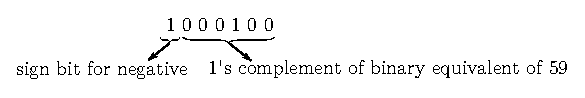
\includegraphics{chap5/div23.eps}
\end{figure}

\begin{note}
1's complement of binary number is simply obtained by replacing 0's by 1's and 1's by 0's.
\end{note}

In sign-2's complement system, $+59$ is represented as,
\begin{figure}[H]
\centering
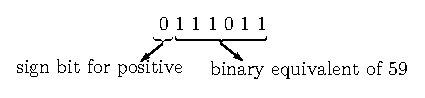
\includegraphics{chap5/div24.eps}
\end{figure}

Thus, for positive number the representation is same in both sign-1's complement and sign-2's complement systems.

But $-59$ is represented as,
\begin{figure}[H]
\centering
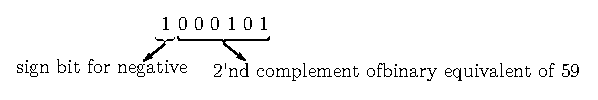
\includegraphics{chap5/div25.eps}
\end{figure}

\begin{note}
2's complement of a binary number is simply obtained by leaving all least significant zeros, the first least significant 1 unchanged and then replacing 1's by 0's and 0's by 1's.
\end{note}

\itheading{Subtraction using 1's complement}

\smallskip
The procedures for subtraction using 1's complement are explained below~:

Say, we want to perform M $-$ N (both M and N are positive numbers). The steps to be followed are,
\begin{itemize}
\item[(i)] Add the minuend M to the 1's complement of subtrahend N.

\item[(ii)] Inspect the result obtained in step (i) for an end carry.
\begin{itemize}
\item[(a)] If an end carry occurs, add 1 to the least significant bit (end around carry).

\item[(b)] If an end carry does not occur, take 1's complement of the number obtained in step (i) and place a negative sign in front of it.
\end{itemize}
\end{itemize}

Consider that we want to perform $58-34$.
\begin{figure}[H]
\centering
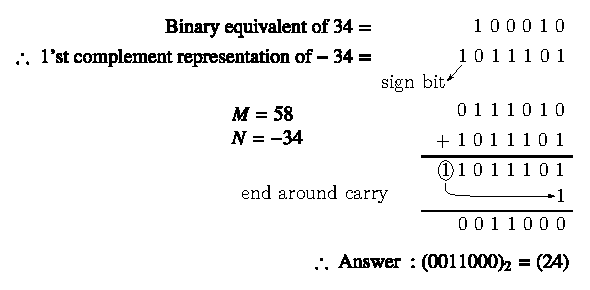
\includegraphics{chap5/div26.eps}
\end{figure}

Now consider $78-90$
\begin{figure}[H]
\centering
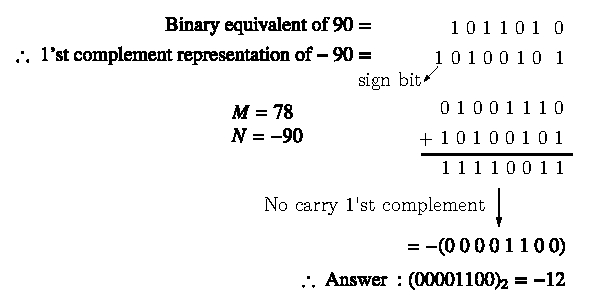
\includegraphics{chap5/div27.eps}
\end{figure}

\itheading{Subtraction using 2's complement}

\smallskip
The procedures for subtraction using 2's complement are explained below~:

Say, we want to perform M $-$ N (both M and N are positive numbers). The steps to be followed are,
\begin{itemize}
\item[(i)] Add the minuend M to the 2's complement of the subtrahend N.

\item[(ii)] Inspect the result obtained in step (i) for an end carry.
\begin{itemize}
\item[(a)] If an end carry occurs, discard it.

\item[(b)] If an end carry does not occur, take the 2's complement of the number obtained in step (i) and place a negative sign in front of it.
\end{itemize}
\end{itemize}

Consider that we want to perform $78-69$.
\begin{figure}[H]
\centering
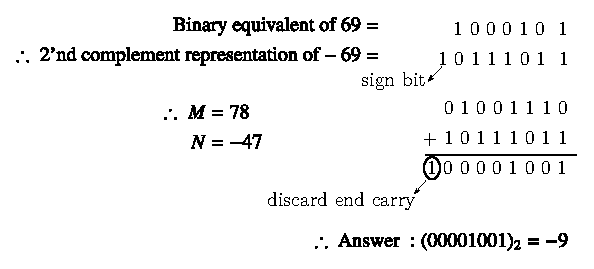
\includegraphics{chap5/div28.eps}
\end{figure}

Now consider $78-84$.
\begin{figure}[H]
\centering
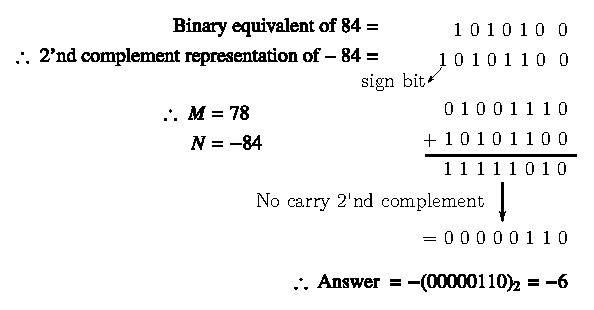
\includegraphics{chap5/div29.eps}
\end{figure}

\eject

\begin{center}
\rule{4cm}{1pt}\\
{\bf\Large Problems}\\[-3pt]
\rule{4cm}{1pt}
\end{center}

\begin{problem}\label{prob5.28}
Perform the following subtractions using 1's complement. Numbers are given in decimal.

\smallskip
(i)~ $47-40$\hfil (ii)~ $505-470$\hfil (iii)~ $39-48$\hfil (iv)~ $2003-2003$
\end{problem}

\begin{solution}
\begin{itemize}
\item[(i)] $47-40$
%\begin{center}
%\begin{tabular}{r@{\qquad}r}
%Binary equivalent of 40 = & 1 0 1 0 0 0\\[3pt]
%$\therefore$~ 1's complement representation of $-40$ = & 1 0 1 0 1 1 1
%\end{tabular}
%\end{center}
\begin{figure}[H]
\centering
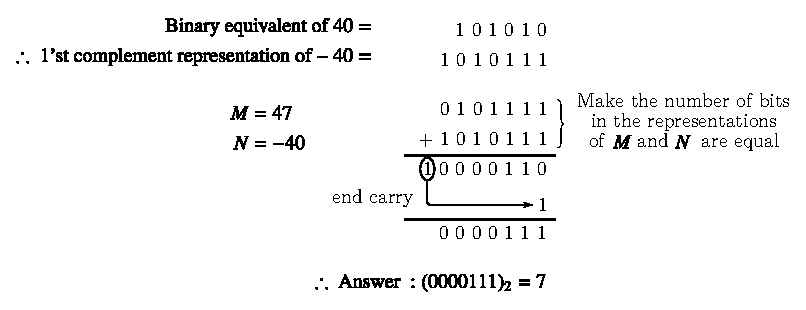
\includegraphics{chap5/div30.eps}
\end{figure}

\item[(ii)] $505-470$
\begin{figure}[H]
\centering
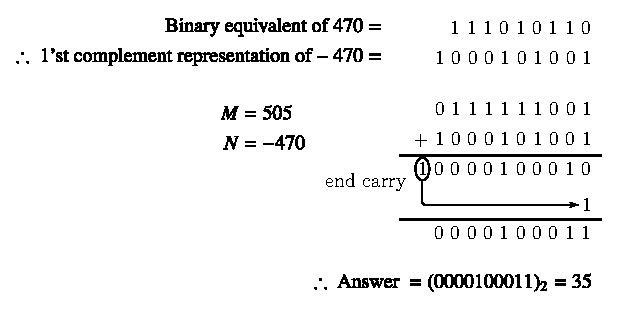
\includegraphics{chap5/div31.eps}
\end{figure}

\eject

\item[(iii)] $39-48$
\begin{figure}[H]
\centering
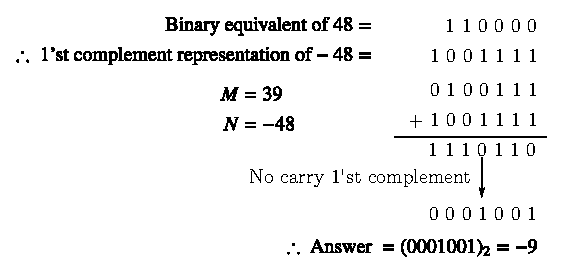
\includegraphics[scale=.97]{chap5/div32.eps}
\end{figure}

\item[(iv)] $2003-2003$
%\begin{center}
%\begin{tabular}{r@{\qquad}r}
%Binary equivalent of 2003 = & 1 1 1 1 1 0 1 0 0 1 1\\[3pt]
%1's complement representation of $-2003$ = & 1 0 0 0 0 0 1 0 1 1 0 0
%\end{tabular}
%\end{center}
\begin{figure}[H]
\centering
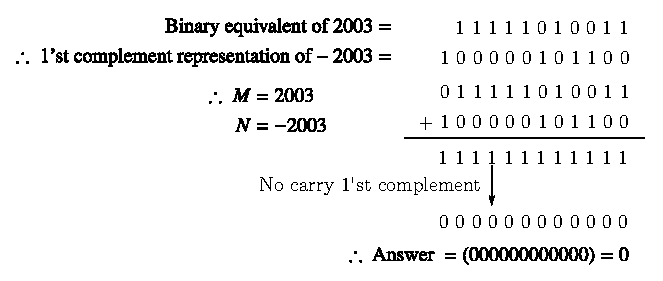
\includegraphics[scale=.97]{chap5/div33.eps}
\end{figure}
\end{itemize}
\end{solution}

\begin{problem}\label{prob5.29}
Perform the subtraction with the following binary numbers using 1's complement.
\begin{center}
\begin{tabular}{r@{\;\,}l@{\qquad\quad}r@{\;\,}l}
(i) & 1 1 0 1 0 $-$ 1 1 0 1 & (ii) & 1 0 0 1 0 $-$ 1 0 0 1 1\\[4pt] 
(iii) & 1 1 0 1 0 $-$ 1 0 0 0 0 & (iv) & 1 0 0 $-$ 1 1 0 0 0 0 
\end{tabular}
\end{center}
\end{problem}

\begin{solution}
Note : In all the cases, the number of bits in the representation of M and N should be made equal.
\begin{itemize}
\item[(i)] 1 1 0 1 0 $-$ 1 1 0 1
\begin{figure}[H]
\centering
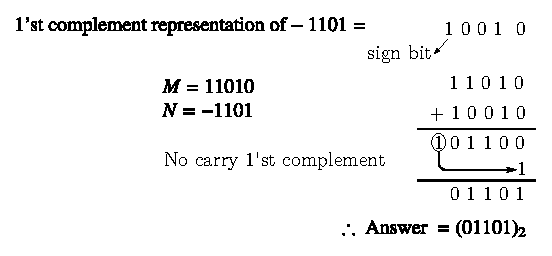
\includegraphics{chap5/div34.eps}
\end{figure}

\item[(ii)] 1 0 0 1 0 $-$ 1 0 0 1 1
\begin{figure}[H]
\centering
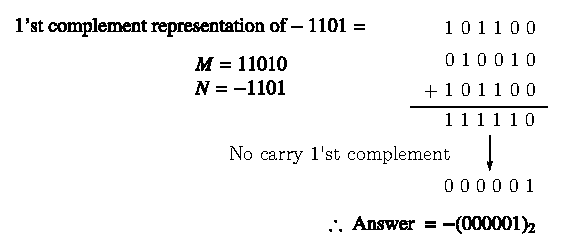
\includegraphics{chap5/div35.eps}
\end{figure}

\item[(iii)] 1 1 0 1 0 $-$ 1 0 0 0 0
\begin{figure}[H]
\centering
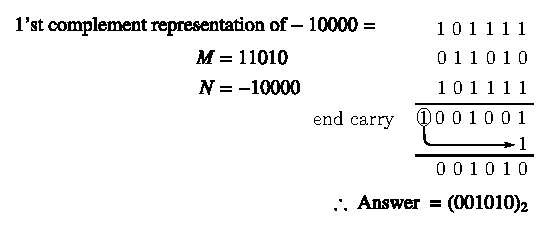
\includegraphics{chap5/div36.eps}
\end{figure}

\item[(iv)] 1 0 0 $-$ 1 1 0 0 0 0
\begin{figure}[H]
\centering
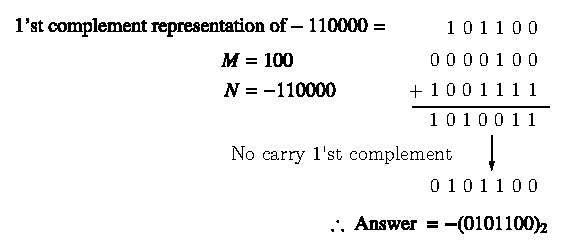
\includegraphics{chap5/div37.eps}
\end{figure}
\end{itemize}
\end{solution}

\begin{problem}\label{prob5.30}
Perform the following subtractions using 2's complement. Numbers are given in decimal.

\smallskip
(i)~ $78-65$\hfil (ii)~ $708-648$\hfil (iii)~ $24-36$\hfil (iv)~ $1029-1029$
\end{problem}

\eject

\begin{solution}
\begin{itemize}
\item[(i)] $78-65$
\begin{figure}[H]
\centering
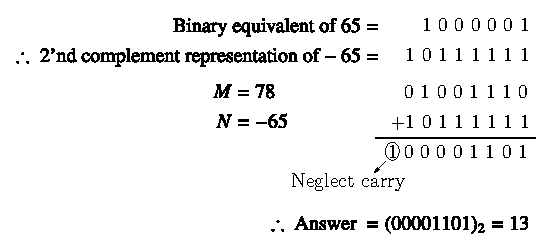
\includegraphics{chap5/div38.eps}
\end{figure}

\item[(ii)] $708-648$
\begin{figure}[H]
\centering
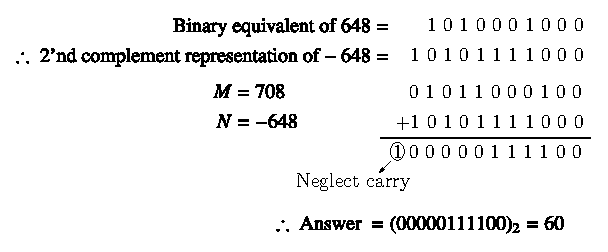
\includegraphics{chap5/div39.eps}
\end{figure}

\item[(iii)] $24-36$
\begin{figure}[H]
\centering
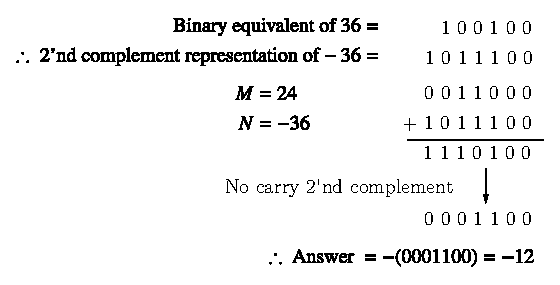
\includegraphics{chap5/div40.eps}
\end{figure}

\eject

\item[(iv)] $1029-1029$
\begin{figure}[H]
\centering
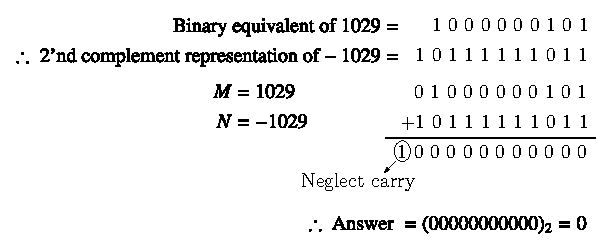
\includegraphics{chap5/div41.eps}
\end{figure}
\end{itemize}
\end{solution}

\begin{problem}\label{prob5.31}
Perform the subtraction with the following binary numbers using 2's complements.
\begin{center}
\begin{tabular}{r@{\;\,}l@{\qquad\quad}r@{\;\,}l}
(i) & 1 1 0 1 0 $-$ 1 1 0 1 & (ii) & 1 0 0 1 0 $-$ 1 0 0 1 1\\[3pt]
(iii) & 1 1 0 1 0 $-$ 1 0 0 0 0 & (iv) & 1 0 0 $-$ 1 1 0 0 0 0
\end{tabular}
\end{center}
\end{problem}

\begin{solution}
\begin{itemize}
\item[(i)] 1 1 0 1 0 $-$ 1 1 0 1
\begin{figure}[H]
\centering
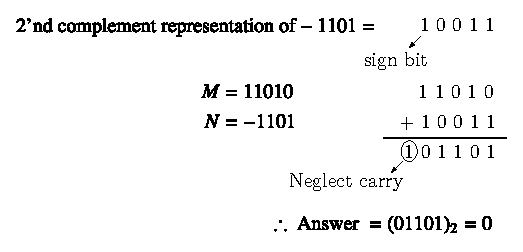
\includegraphics{chap5/div42.eps}
\end{figure}

\item[(ii)] 1 0 0 1 0 $-$ 1 0 0 1 1
\begin{figure}[H]
\centering
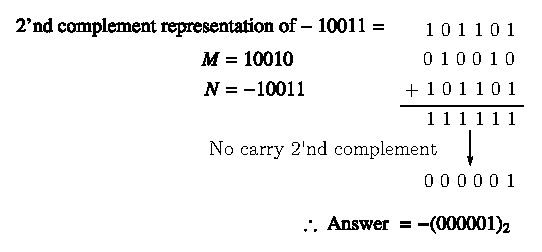
\includegraphics{chap5/div43.eps}
\end{figure}

\eject

\item[(iii)] 1 1 0 1 0 $-$ 1 0 0 0 0
\begin{figure}[H]
\centering
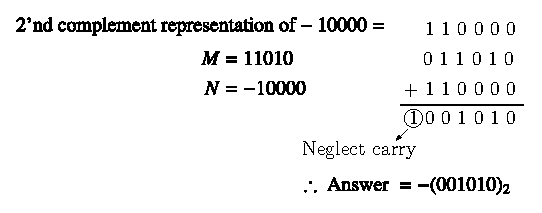
\includegraphics{chap5/div44.eps}
\end{figure}

\item[(iv)] 1 0 0 $-$ 1 1 0 0 0 0
\begin{figure}[H]
\centering
\includegraphics{chap5/div45.eps}
\end{figure}
\end{itemize}
\end{solution}

\section{Addition in other number systems}\label{sec7.7}

\heading{(i) {\em Addition in octal system}}

The addition in octal system can be performed by the same way as in the decimal system. Add the digits in each column in decimal and convert this sum into octal. Write the sum in that column and carry the carry term to the next higher significant column.

For example, add $(334.65)_{8}$ to $(671.14)_{8}$
\begin{figure}[H]
\centering
\includegraphics{chap5/div46.eps}
\end{figure}

\noindent
$\therefore$~ Answer $= (1226.01)_{8}$.

\smallskip
\heading{(ii) {\em Addition in hexadecimal system}}

The addition in hexadecimal system can also be carried out by the same way. i.e., add the digits in each column in decimal and convert this sum into hexadecimal. Write the sum in that column and carry the carry term to the higher significant column.

For example, add (7AB.67)$_{16}$  to (15C.71)$_{16}$
\begin{figure}[H]
\centering
\includegraphics{chap5/div47.eps}
\end{figure}

\noindent
$\therefore$~ Answer = (907.D8)$_{16}$.

\begin{center}
\rule{4cm}{1pt}\\
{\bf\Large Problems}\\[-3pt]
\rule{4cm}{1pt}
\end{center}

\begin{problem}\label{prob5.32}
Add the following octal numbers.
\begin{center}
\begin{tabular}{r@{\;\,}l@{\qquad}r@{\;\,}l@{\qquad}r@{\;\,}l}
(i) & $173+265$ & (ii) & $1247-2053$ & (iii) & $25.76+16.57$\\[3pt]
(iv) & $273.56+425.07$ & (v) & $74632.002+652.02$ &
\end{tabular}
\end{center}
\end{problem}

\medskip
\begin{solution}
\begin{itemize}
\item[(i)] 
$173+265$

\begin{tabular}{rcccc}
 & {\footnotesize 1} & {\footnotesize 1} & &\\
 & 1 & 7 & 3&\\
+ & 2 & 6 & 5&\\
\cline{2-4}
 & 4 & 6 & 0&\\[10pt]
\multicolumn{5}{l}{$\therefore~(173)_{8}+(265)_{8}=(460)_{8}$}
\end{tabular}

\item[(ii)] 
$1247+2053$

\begin{tabular}{rccccc}
 & {\footnotesize 0} & {\footnotesize 1} & {\footnotesize 1} & &\\
 & 1 & 2 & 4 & 7 &\\
+ & 2 & 0 & 5 & 3 &\\
\cline{2-5}
 & 3 & 3 & 2 & 2 &\\[10pt]
\multicolumn{6}{l}{$\therefore~(1247)_{8}+(2053)_{8}=(3322)_{8}$}
\end{tabular}


\medskip

\item[(iii)] $25.76+16.57$

\begin{tabular}[t]{rcccccc}
 & {\footnotesize 1} & {\footnotesize 1} & & {\footnotesize 1} & &\\
 & 2 & 5 & . & 7 & 6 & \\
+ & 1 & 6 & . & 5 & 7 &\\
\cline{2-6}
 & 4 & 4 & . & 5 & 5 &\\[10pt]
\multicolumn{7}{l}{$\therefore~(25.76)_{8}+(16.57)_{8}=(44.55)_{8}$}
\end{tabular}

\item[(iv)]
$273.56+425.07$

\begin{tabular}[t]{rccccccc}
 & {\footnotesize 1} & {\footnotesize 1} & {\footnotesize 0} & & {\footnotesize 1} & &\\
 & 2 & 7 & 3 & . & 5 & 6 &\\
+ & 4 & 2 & 5 & . & 0 & 7\\
\cline{2-6}
 & 7 & 2 & 0 & . & 6 & 5 &\\[10pt]
\multicolumn{8}{l}{$\therefore~(273.56)_{8}+(425.07)_{8}=(720.65)_{8}$}
\end{tabular}

\item[(v)] $74632.002+652.02$

\begin{tabular}{rcccccccccc}
 & {\footnotesize 0} & {\footnotesize 1} & {\footnotesize 1} & {\footnotesize 0} & {\footnotesize 0} & & {\footnotesize 0} & {\footnotesize 0} & &\\
 & 7 & 4 & 6 & 3 & 2 & . & 0 & 0 & 2 &\\
+ & & & 6 & 5 & 2 & . & 0 & 2 &&\\
\cline{2-10}
 & 7 & 5 & 5 & 0 & 4 & . & 0 & 2 & 2 &\\[10pt]
\multicolumn{11}{l}{$\therefore~ (74632.002)_{8}+(652.02)_{8}=(75504.022)_{8}$}
\end{tabular}
\end{itemize}
\end{solution}

\begin{problem}
Add the following hexadecimal numbers.
\begin{itemize}
\item[(i)] AC6 + B59

\item[(ii)] A0FC + B75F

\item[(iii)] E0F3.5D + 49E6.F7

\item[(iv)] AA.BB + 10.7E

\item[(v)] E0F3.47 + 41.3
\end{itemize}
\end{problem}

\begin{solution}
\begin{itemize}
\item[(i)] AC6 + B59

\begin{tabular}{rccc}
{\footnotesize 1} & {\footnotesize 1} & {\footnotesize 0} &\\
 & A & C & 6\\
+ & B & 5 & 9\\
\hline
1 & 6 & 1 & F
\end{tabular}

\medskip
$\therefore$~ (AC6)$_{16}$ + (B59)$_{16}$ = (161F)$_{16}$

\item[(ii)] A0FC + B75F

\begin{tabular}{ccccc}
{\footnotesize 1} & {\footnotesize 0} & {\footnotesize 1} & {\footnotesize 1} & \\
 & A & 0 & F & C \\
+ & B & 7 & 5 & F\\
\hline
1 & 5 & 8 & 5 & B
\end{tabular}

\medskip
$\therefore$~ (A0FC)$_{16}$ + (B75F)$_{16}$ = (1585B)$_{16}$

\item[(iii)] E0F3.5D + 49E6.F7

\begin{tabular}{cccccccc}
{\footnotesize 1} & {\footnotesize 0} & {\footnotesize 1} & {\footnotesize 0} & {\footnotesize 1} & & {\footnotesize 1} &\\
 & E & 0 & F & 3 & . & 5 & D\\
+ & 4 & 9 & E & 6 & . & F & 7\\
\hline
1 & 2 & A & D & A & . & 5 & 4
\end{tabular}

\medskip
$\therefore$~ (E0F3.5D)$_{16}$ + (49E6.F7)$_{16}$ = (12ADA.54)$_{18}$

\item[(iv)] AA.BB + 10.7E

\begin{tabular}{cccccc}
 & {\footnotesize 0} & {\footnotesize 1} & & {\footnotesize 1} &\\
 & A & A & . & B & B\\
+ & 1 & 0 & . & 7 & E\\
\cline{2-5}
 & B & B & . & 3 & 9
\end{tabular}

\medskip
$\therefore$~ (AA.BB)$_{16}$ + (10.7E)$_{16}$ = (BB.39)$_{16}$

\item[(v)] E0F3.47 + 41.3

\begin{tabular}{cccccccc}
 & {\footnotesize 0} & {\footnotesize 1} & {\footnotesize 0} & {\footnotesize 0} & & {\footnotesize 0} & \\
 & E & 0 & F & 3 & . & 4 & 7\\
+ & & & 4 & 1 & . & 3 & \\
\cline{2-8}
\end{tabular}

\medskip
$\therefore$~ (E0F3.47)$_{16}$ + (41.3)$_{16}$ = (E134.77)$_{16}$
\end{itemize}
\end{solution}

\section{Subtraction in other number systems}\label{sec5.8}

\heading{(i)~ {\em Subtraction in octal system}}

Subtraction in octal system can be performed by using either 7's or 8's complement method. The 7's complement of an octal number may be obtained by subtracting each digit of that number from 7. To obtain 8's complement of an octal number, add 1 to it's 7's complement.

\smallskip
\heading{Subtraction by 7's complement method :} The steps for subtraction in octal system, using 7's complement method are as follows. Remember that the number of digits in a minuend and subtrahend must be equal.
\begin{description}
\item[Step 1~:] Find the 7's complement of subtrahend.

\item[Step 2~:] Add two octal numbers (i.e., minuend and 7's complement of subtrahend).

\item[Step 3~:] 
\begin{itemize}
\item[(a)] If an end carry occurs, add 1 to the least significant digit.

\item[(b)] If an end carry does not occur, take 7's complement of the number obtained in step 2 and place a negative sign in front of it.
\end{itemize}
\end{description}

\heading{Subtraction by 8's complement method~:} The steps for subtraction in octal system using 8's complement method are as follows. Remember that the number of digits in minuend and subtrahend must be equal.
\begin{description}
\item[Step 1~:] Find the 8's complement of subtrahend.

\item[Step 2~:] Add two octal numbers (i.e., minuend and 8's complement of subtrahend.

\item[Step 3~:] 
\begin{itemize}
\item[(a)] If an end carry occurs, discard it.

\item[(b)] If an end carry does not occur, take 8's complement of the number obtained in step 2 and place a negative sign in front of it.
\end{itemize}
\end{description}

\begin{center}
\rule{4cm}{1pt}\\
{\bf\Large Problems}\\[-3pt]
\rule{4cm}{1pt}
\end{center}

\begin{problem}\label{prob5.34}
Subtract $(5425.65)_{8}$ from $(267.51)_{8}$ using 7's complement method.
\end{problem}

\begin{solution} Minuend = $(257.51)_{8}$

\qquad\!Subtrahend = $(5425.65)_{8}$

\smallskip
7's complement of subtrahend = $(2352.12)_{8}$

Now
\begin{center}
\begin{tabular}{rccccccc}
 & 0 & 2 & 6 & 7 & . & 5 & 1\\
+ & 2 & 3 & 5 & 2 & . & 1 & 2\\
\cline{2-8}
No end carry & 2 & 6 & 4 & 1 & . & 6 & 3
\end{tabular}
\end{center}
Since, end carry does not occur, take 7's complement of $(2641.63)_{8}$ and place negative sign in front of it.

$\therefore$~ Answer = $-(5136.14)_{8}$.
\end{solution}

\eject

\begin{problem}\label{prob5.35}
Subtract $(5425.65)_{8}$ from $(267.51)_{8}$ using 8's complement method.
\end{problem}

\begin{solution}
Minuend = $(0267.51)_{8}$

\qquad\!Subtrahend = $(5425.65)_{8}$

\smallskip
8's complement of subtrahend = 7's complement of subtrahend + 1


\medskip
\begin{tabular}{@{\hspace{4.75cm}}rrr}
 = && 2 3 5 2 . 1 2\\
   & + & 1\\
\cline{2-3}
 & & (2 3 5 2 . 1 3)$_{8}$\!\!\!\!\!
\end{tabular}

\smallskip
Now
\begin{center}
\begin{tabular}{rccccccc}
 & 0 & 2 & 7 & . & 5 & 1\\[3pt]
+ & 2 & 3 & 5 & 2 & . & 1 & 3\\
\cline{2-8}
No end carry & 2 & 6 & 4 & 1 & . & 6 & 4
\end{tabular}
\end{center}
Since end carry does not occur, take 8's complement of $(2641.64)_{8}$ and place negative sign in front of it.

\medskip
\begin{tabular}{rr}
$\therefore$~ 8's complement of $(2641.64)_{8}$ is = & 5  1  3  6 . 1  3\\
 + & 1\\
\cline{2-2}
 & (5 1 3 6 . 1 4)$_{8}$\!\!\!\!
\end{tabular}
\smallskip

$\therefore$~ Answer = $-(5136.14)_{8}$
\end{solution}

\begin{problem}\label{prob5.36}
Subtract $(2347.15)_{8}$ from $(6573.16)_{8}$ using 7's complement method.
\end{problem}

\begin{solution}
Minuend = $(6573.16)_{8}$

\qquad\!Subtrahend = $(2347.15)_{8}$

\smallskip
7's complement of subtrahend = $(5430.62)_{8}$
\begin{figure}[H]
\centering
\includegraphics{chap5/div48.eps}
\end{figure}
\end{solution}

\begin{problem}\label{prob5.37}
Subtract $(2347.15)_{8}$ from $(6573.16)_{8}$ using 8's complement method.
\end{problem}

\begin{solution}
Minuend = $(6573.16)_{8}$

\qquad\!Subtrahend = $(2347.15)_{8}$
\medskip

\begin{tabular}{rr}
8's complement of subtrahend = & 5 4 3 0 . 6 2\\
+ & 1\\
\cline{2-2}
 & (5 4 3 0 . 6 3)$_{8}$\!\!\!\!
 \end{tabular}

\eject

Now
\begin{center}
\tabcolsep=4pt
\begin{tabular}{rcccccccc}
 && 6 & 5 & 7 & 3 & . & 1 & 6\\
&+ & 5 & 4 & 3 & 0 & . & 6 & 3\\
\cline{2-9}
end carry & \mycirc{1} & 4 & 2 & 2 & 4 & . & 0 & 1
\end{tabular}
\end{center}

Here, an end carry occurs, so discard it.

$\therefore$~ Answer = $(4224.01)_{8}$.
\end{solution}

\begin{problem}\label{prob5.38}
Subtract $(4317.64)_{8}$ from $(42.345)_{8}$ using
\begin{itemize}
\item[(i)] 7's complement method.

\item[(ii)] 8's complement method.
\end{itemize}
\end{problem}

\begin{solution}
Minuend = $(0042.345)_{8}$

\qquad\!Subtrahend = $(4317.640)_{8}$
\begin{itemize}
\item[(i)] Using 7's complement method.

7's complement of subtrahend = $(3460.137)_{8}$

Now
\begin{center}
\begin{tabular}{rcccccccc}
 & 0 & 0 & 4 & 2 & . & 3 & 4 & 5\\
+ & 3 & 4 & 6 & 0 & . & 1 & 3 & 7\\
\cline{2-8}
No end carry & 3 & 5 & 2 & 2 & . & 5 & 0 & 4
\end{tabular}
\end{center}
Here, an end carry does not occur. So take the 7's complement of $(3522.504)_{8}$ and place negative sign in front of it.

$\therefore$~ Answer = $(4255.273)_{8}$.

\item[(ii)] Using 8's complement method.

8's complement of subtrahend = 7's complement of subtrahend ${}+1$
\begin{center}
\begin{tabular}{rrrc@{\hspace{.22cm}}}
= && 3  4  6  0  .  1  3  7 &\\
& + & 1&\\
\cline{3-3}
 && (3 4 6 0 . 1 4 0)$_{8}$\!\!\!\! & 
\end{tabular}
\end{center}

Now
\begin{center}
\tabcolsep=4pt
\begin{tabular}{rcccccccc}
 & 0 & 0 & 4 & 2 & . & 3 & 4 & 5\\
+ & 3 & 4 & 6 & 0 & . & 1 & 4 & 0\\
\cline{2-9}
No end carry & 3 & 5 & 2 & 2 & . & 5 & 0 & 5
\end{tabular}
\end{center}
Here, and end carry does not occur. So take 8's complement of $(3522.505)_{8}$ and add negative sign in front of it.

\medskip
\begin{tabular}{rr}
8's complement of $(3522.505)_{8}$ = & 4 2 5 5 . 2 7 2\\
+ & 1\\
\cline{2-2}
 & (4 2 5 5 . 2 7 3)$_{8}$\!\!\!\!
\end{tabular}

$\therefore$~ Answer = ${}-(4255.273)_{8}$.
\end{itemize}
\end{solution}

\begin{problem}\label{prob5.39}
Subtract $(146.736)_{8}$ from $(2347.051)_{8}$ using
\begin{itemize}
\item[(i)] 7's complement method.

\item[(ii)] 8's complement method.
\end{itemize}
\end{problem}

\begin{solution}
Minuend = $(2347.051)_{8}$

\qquad\!Subtrahend = $(0146.736)_{8}$
\begin{itemize}
\item[(i)] Using 7's complement method

7's complement of subtrahend = $(7631.041)_{8}$
\begin{figure}[H]
\centering
\includegraphics{chap5/div49.eps}
\end{figure}

$\therefore$~ Answer $=(2200.113)_{8}$

\item[(ii)] Using 8's complement method

8's complement of subtrahend = 7's complement of subtrahend ${}+1$

\smallskip
\begin{tabular}{@{\hspace{4.75cm}}rr}
= & 7 6 3 1 . 0 4 1\\
+ & 1\\
\cline{2-2}
 & (7 6 3 1 . 0 4 2)$_{8}$\!\!\!\!
\end{tabular}

Now
\begin{center}
\tabcolsep=4pt
\begin{tabular}{rccccccccc}
 & & 2 & 3 & 4 & 7 & . & 0 & 5 & 1\\
 & + & 7 & 6 & 3 & 1 & . & 0 & 4 & 2\\
\cline{2-10}
end carry & \mycirc{1} & 2 & 3 & 0 & 0 & . & 1 & 1 & 3
\end{tabular}
\end{center}
Here an end carry occurs. So discard it.

$\therefore$~ Answer = $(2200.113)_{8}$.
\end{itemize}
\end{solution}

\heading{(ii) {\em Subtraction in hexadecimal system~:}}

Subtraction in hexadecimal system can be performed by using either 15's complement or 16's complement method. The 15's complement of a hexadecimal number may be obtained by subtracting each digit of that number by 15 (i.e., F). To obtain 16's complement of a hexadecimal number, add 1 to its 15's complement.

\smallskip
\heading{Subtraction by 15's complement method~:} The steps for subtraction in hexadecimal system using 15's complement method are as follows. Remember that the number of digits in minuend and subtrahend must be equal.
\begin{description}
\item[Step 1~:] Find the 15's complement of subtrahend.

\item[Step 2~:] Add two hexadecimal numbers (i.e., minuend and 15's complement of subtrahend).

\item[Step 3~:] 
\begin{itemize}
\item[(a)] If an end carry occurs, add 1 to the least significant digit.

\item[(b)] If an end carry does not occur, take 15's complement of the number obtained in step 2 and place a negative sign in front of it.
\end{itemize}
\end{description}

\heading{Subtraction by 16's complement method~:} The steps for subtraction in hexadecimal system using 16's complement method are as follows. Remember that the number of digits in minuend and subtrahend must be equal.
\begin{description}
\item[Step 1~:] Find the 16s complements of subtrahend.

\item[Step 2~:] Add two hexadecimal numbers (i.e., minuend and 16's complement of subtrahend).

\item[Step 3~:] 
\begin{itemize}
\item[(a)] If an end carry occurs, discard it.

\item[(b)] If an end carry does not occur, take 16's complement of the number obtained in step 2 and place a negative sign in front of it.
\end{itemize}
\end{description}

\eject

\begin{center}
\rule{4cm}{1pt}\\
{\bf\Large Problems}\\[-3pt]
\rule{4cm}{1pt}
\end{center}

\begin{problem}\label{prob5.40}
Subtract (A68.C4)$_{16}$ from (B74.AB)$_{16}$ using
\begin{itemize}
\item[(i)] 15's complement method.

\item[(ii)] 16's complement method.
\end{itemize}
\end{problem}

\begin{solution}
Minuend = (B74.AB)$_{16}$

\qquad\!Subtrahend = (A68.C4)$_{16}$
\begin{itemize}
\item[(i)] Using 15's complement method

\smallskip
15's complement of subtrahend = (5 9 7 . 3 B)$_{16}$
\begin{figure}[H]
\centering
\includegraphics{chap5/div50.eps}
\end{figure}
%$\therefore$~ Answer = (10B.E7)$_{16}$.

\item[(ii)] Using 16's complement method.

16's complement of subtrahend = 15's complement of subtrahend ${}+1$

\smallskip
\begin{tabular}{@{\hspace{4.95cm}}rr}
= & 5 9 7 . 3 B\\
+ & 1\\
\cline{2-2}
 & 5 9 7 . 3 C
\end{tabular}

Now
\begin{center}
\tabcolsep=4pt
\begin{tabular}{rccccccc}
 & & B & 7 & 4 & . & A & B\\
 & + & 5 & 9 & 7 & . & 3 & C\\
\cline{2-8}
end carry & \mycirc{1} & 1 & 0 & B & . & E & 7
\end{tabular}
\end{center}
Here, an end carry occurs. So discard it.

$\therefore$~ Answer = (10B.E7)$_{16}$.
\end{itemize}
\end{solution}

\eject

\begin{problem}\label{prob5.41}
Perform the following using 15's complement method.
\begin{itemize}
\item[(a)] (74A)$_{16}$ $-$ (84C)$_{16}$

\item[(b)] (1B76)$_{16}$ $-$ (4A)$_{16}$

\item[(c)] (3A47.C8)$_{16}$ $-$ (743.4AC)$_{16}$

\item[(d)] (47A.6)$_{16}$ $-$ (187A.43)$_{16}$
\end{itemize}
\end{problem}

\begin{solution}
\begin{itemize}
\item[(a)] (74A)$_{16}$ $-$ (84C)$_{16}$
\begin{center}
\begin{tabular}{r@{\;=\;}l}
Minuend & (74A)$_{16}$\\[3pt]
Subtrahend & (84C)$_{16}$
\end{tabular}
\end{center}
15's complement of subtrahend = (7B3)$_{16}$

Now
\begin{center}
\tabcolsep=4pt
\begin{tabular}{rccc}
 & 7 & 4 & A\\
+ & 7 & B & 3\\
\cline{2-4}
no end carry & E & F & D
\end{tabular}
\end{center}
Here, no end carry occurs. So take 15's complement of (EFD)$_{16}$ and place negative sign in front of it.

$\therefore$~ Answer = ${}-(102)_{16}$.

\item[(b)] (1B76)$_{16}$ $-$ (4A)$_{16}$
\begin{center}
\begin{tabular}{r@{\;=\;}l}
Minuend & (1B76)$_{16}$\\[3pt]
Subtrahend & (004A)$_{16}$
\end{tabular}
\end{center}
15's complement of subtrahend = (FFB5)$_{16}$
\begin{figure}[H]
\centering
\includegraphics{chap5/div51.eps}
\end{figure}
%$\therefore$~ Answer = (1B2C)$_{16}$

\eject

\item[(c)] (3A47.C8)$_{16}$ $-$ (743.4AC)$_{16}$
\begin{center}
\begin{tabular}{r@{\;=\;}l}
Minuend & (3A47.C80)$_{16}$\\[3pt]
Subtrahend & (0743.4AC)$_{16}$
\end{tabular}
\end{center}
15's complement of subtrahend = (F8BC.B53)$_{16}$
\begin{figure}[H]
\centering
\includegraphics{chap5/div52.eps}
\end{figure}
%$\therefore$~ Answer = (3304.7D4)$_{16}$

\item[(d)] (47A.6)$_{16}$ $-$ (187A.43)$_{16}$
\begin{center}
\begin{tabular}{r@{\;=\;}l}
Minuend & (047A.60)$_{16}$\\[3pt]
Subtrahend & (187A.43)$_{16}$
\end{tabular}
\end{center}
15's complement of subtrahend = (E785.BC)$_{16}$.

Now
\begin{center}
\tabcolsep=4pt
\begin{tabular}{rccccccc}
 & 0 & 4 & 7 & A & . & 6 & 0\\
+ & E & 7 & 8 & 5 & . & B & C\\
\cline{2-8}
No end carry & E & C & 0 & 0 & . & 1 & C
\end{tabular}
\end{center}
Here, end carry does not occur. So take 15's complement of (EC00.1C)$_{8}$ and place negative sign in front of it.

$\therefore$~ Answer = $-$ (13FF.E3)$_{16}$.
\end{itemize}
\end{solution}

\begin{problem}\label{prob5.42}
Perform the following using 16's complement method.
\begin{itemize}
\item[(a)] (74A)$_{16}$ $-$ (84C)$_{16}$

\item[(b)] (1B76)$_{16}$ $-$ (4A)$_{16}$

\item[(c)] (3A47.C8)$_{16}$ $-$ (743.4AC)$_{16}$

\item[(d)] (47A.6)$_{16}$ $-$ (187A.43)$_{16}$
\end{itemize}
\end{problem}

\eject

\begin{solution}
\begin{itemize}
\item[(a)] (74A)$_{16}$ $-$ (84C)$_{16}$
\begin{center}
\begin{tabular}{r@{\;=\;}l}
Minuend & (74A)$_{16}$\\
Subtrahend & (84C)$_{16}$
\end{tabular}
\end{center}
16's complement of subtrahend = 15's complement of subtrahend ${}+1$

\smallskip
\begin{tabular}{@{\hspace{4.95cm}}rr}
= & 7 B 3\\
+ & 1\\
\cline{2-2}
 & 7 B 4
\end{tabular}

Now,
\begin{center}
\begin{tabular}{rcccr}
 & 7 & 4 & A &\\
+ & 7 & B & 4 & \\
\cline{2-4}
No end carry & E & F & E & \qquad\qquad
\end{tabular}
\end{center}

Here, an end carry does not occur. So take 16's complement of (EFE)$_{16}$ and place negative sign in front of it.
\begin{center}
\begin{tabular}{rr}
16's complement of (EFE)$_{16}$ = & 1  0  1\\
                + &  1\\
\cline{2-2}
 & 1 0  2
\end{tabular}
\end{center}
$\therefore$~ Answer = ${}-(102)_{16}$.

\item[(b)] (1B76)$_{16}$ = (4A)$_{16}$
\begin{center}
\begin{tabular}{r@{\;=\;}l}
Minuend & (1B76)$_{16}$\\
Subtrahend & (004A)$_{16}$
\end{tabular}
\end{center}
16's complement of subtrahend = 15's complement of subtrahend ${}+1$

\smallskip
\begin{tabular}{@{\hspace{4.95cm}}rr}
= & F F B 5\\
+ & 1\\
\cline{2-2}
 & (F F B 6)$_{16}$\!\!\!\!\!\!
\end{tabular}

Now,
\begin{center}
\tabcolsep=4pt
\begin{tabular}{rccccc}
 && 1 & B & 7 & 6\\
 & + & F & F & B & 6\\
\cline{2-6}
end carry & \mycirc{1} & 1 & B & 2 & C
\end{tabular}
\end{center}
Here, an end carry occurs. So discard it.

$\therefore$~ Answer = (1B2C)$_{16}$.

\item[(c)] (3A47.C8)$_{16}$ $-$ (743.4AC)$_{16}$
\begin{center}
\begin{tabular}{r@{\;=\;}l}
Minuend & (3A47.C80)$_{16}$\\
Subtrahend & (0743.4AC)$_{16}$
\end{tabular}
\end{center}
16's complement of subtrahend = 15's complement of subtrahend ${}+1$
\smallskip

\begin{tabular}{@{\hspace{4.95cm}}rr}
= & F 8 B C . B 5 3\\
+ & 1\\
\cline{2-2}
 & F 8 B C . B 5 4
\end{tabular}

Now
\begin{center}
\tabcolsep=4pt
\begin{tabular}{rc@{\,}cccccccc}
 & & 3 & A & 4 & 7 & . & C & 8 & 0\\
+ & & F & 8 & B & C & . & B & 5 & 4\\
\cline{3-10}
end carry & \mycirc{1} & 3 & 3 & 0 & 4 & . & 7 & D & 4
\end{tabular}
\end{center}
Here, and end carry occurs. So discard it.

$\therefore$~ Answer = (3304.7D4)$_{16}$.

\item[(d)] (47A.6)$_{16}$ $-$ (187A.43)$_{16}$.
\begin{center}
\begin{tabular}{r@{\;=\;}l}
Minuend & (047A.60)$_{16}$\\
Subtrahend & (187A.43)$_{16}$
\end{tabular}
\end{center}
16's complement of subtrahend = 15's complement of subtrahend ${}+1$.

\smallskip
\begin{tabular}{@{\hspace{2cm}}rr}
= & E 7 8 5 . B C\\
+ & 1\\
\cline{2-2}
 & (E 7 8 5 . B D)$_{16}$
\end{tabular}

Now,
\begin{center}
\tabcolsep=4pt
\begin{tabular}{rccccccc}
 & 0 & 4 & 7 & A & . & 6 & 0\\
+ & E & 7 & 8 & 5 & . & B & D\\
\cline{2-8}
No end carry & E & C & 0 & 0 & . & 1 & D
\end{tabular}
\end{center}
Here, an end carry does not occur. So take 16's complement of (EC00.1D)$_{16}$ and place a negative sign in front of it.

\eject

16's complement of (EC00.1D)$_{16}$ =
\begin{center}
\tabcolsep=3pt
\begin{tabular}{rccccccc}
 & 1 & 3 & F & F & . & E & 2\\
+ & & & & & & & 1\\
\cline{2-8}
 & 1 & 3 & F & F & . & E & 3
\end{tabular}
\end{center}
$\therefore$~ Answer = $-$ (13FF.E3)$_{16}$
\end{itemize}
\end{solution}

\heading{(iii)~ {\em Subtraction in decimal system}}

Subtraction in decimal system can be performed by using either 9's complement or 10's complement method. The 9's complement of a decimal number may be obtained by subtracting each digit of that number from 9. To obtain 10's complement of a decimal number, add 1 to its 9's complement.

\smallskip
\heading{Subtraction by 9's complement method~:} The steps for subtraction in decimal system using 9's complement method are as follows. Remember that the number of digits in minuend and subtrahend must be equal.
\begin{description}
\item[Step 1~:] Find the 9's complement of subtrahend.

\item[Step 2~:] Add two decimal numbers (i.e., minuend and 9's complement of subtrahend).

\item[Step 3~:] 
\begin{itemize}
\item[(a)] If an end carry occurs, add 1 to the least significant digit.

\item[(b)] If an end carry does not occur, take 9's complement of the number obtained in step 2 and place a negative sign in front of it.
\end{itemize}
\end{description}

\heading{Subtraction by 10's complement method~:} The steps for subtraction in decimal system using 10's complement method are as follows. Remember that the number of digits in minuend and subtrahend must be equal.
\begin{description}
\item[Step 1~:] Find the 10's complement of subtrahend.

\item[Step 2~:] Add two decimal numbers. (i.e., minuend and 10's complement of subtrahend).

\item[Step 3~:]
\begin{itemize}
\item[(a)] If an end carry occurs, discard it.

\item[(b)] If an end carry does not occur, take 10's complement of the number obtained in step 2 and place a negative sign in front it.
\end{itemize}
\end{description}

\eject

\begin{center}
\rule{4cm}{1pt}\\
{\bf\Large Problems}\\[-3pt]
\rule{4cm}{1pt}
\end{center}

\begin{problem}\label{prob5.43}
Perform the following using 9's complement method.
\begin{itemize}
\item[(a)] $(487)_{10}-(354)_{10}$

\item[(b)] $(8437)_{10}-(39)_{10}$

\item[(c)] $(309)_{10}-(1447)_{10}$

\item[(d)] $(4357.36)_{10}-(2003.42)_{10}$

\item[(e)] $(357.434)_{10}-(1048.05)_{10}$
\end{itemize}
\end{problem}

\begin{solution}
\begin{itemize}
\item[(a)] $(487)_{10}-(354)_{10}$
\begin{center}
\begin{tabular}{r@{\;=\;}l}
Minuend & $(487)_{10}$\\
Subtrahend & $(354)_{10}$
\end{tabular}
\end{center}
9's complement of subtrahend = $(645)_{10}$.
\begin{figure}[H]
\centering
\includegraphics{chap5/div53.eps}
\end{figure}
%$\therefore$~ Answer $=(133)_{10}$.

\item[(b)] $(8437)_{10}-(39)_{10}$
\begin{center}
\begin{tabular}{r@{\;=\;}l}
Minuend & $(8437)_{10}$\\
Subtrahend & $(0039)_{10}$
\end{tabular}
\end{center}
9's complement of subtrahend = $(9960)_{10}$.
\begin{figure}[H]
\centering
\includegraphics{chap5/div54.eps}
\end{figure}
%$\therefore$~ Answer = $(8398)_{10}$.

\item[(c)] $(309)_{10}-(1447)_{10}$
\begin{center}
\begin{tabular}{r@{\;=\;}l}
Minuend & $(0309)_{10}$\\
Subtrahend & $(1447)_{10}$
\end{tabular}
\end{center}
9's complement of subtrahend = $(8552)_{10}$.

Now,
\begin{center}
\tabcolsep=4pt
\begin{tabular}{rcccc}
 & 0 & 3 & 0 & 9\\
+ & 8 & 5 & 5 & 2\\
\cline{2-5}
No end carry & 8 & 8 & 6 & 1
\end{tabular}
\end{center}
Here, an end carry does not occur. So take 9's complement of $(8861)_{10}$ and place a negative sign in front of it.

$\therefore$~ Answer $=-(1138)_{10}$

\item[(d)] $(4357.36)_{10}-(2003.42)_{10}$
\begin{center}
\begin{tabular}{r@{\;=\;}l}
Minuend & $(4357.36)_{10}$\\
Subtrahend & $(2003.42)_{10}$
\end{tabular}
\end{center}
9's complement of subtrahend = $(7996.57)_{10}$.
\begin{figure}[H]
\centering
\includegraphics{chap5/div55.eps}
\end{figure}
%$\therefore$~ Answer $=(2353.94)_{10}$.

\item[(e)] $(357.434)_{10}-(1048.05)_{10}$
\begin{center}
\begin{tabular}{r@{\;=\;}l}
Minuend & $(0357.434)_{10}$\\
Subtrahend & $(1048.050)_{10}$
\end{tabular}
\end{center}
9's complement of subtrahend = $(8951.949)_{10}$.

Now
\begin{center}
\tabcolsep=4pt
\begin{tabular}{rcccccccc}
 & 0 & 3 & 5 & 7 & . & 4 & 3 & 4\\
+ & 8 & 9 & 5 & 1 & . & 9 & 4 & 9\\
\cline{2-9}
No end carry & 9 & 3 & 0 & 9 & . & 3 & 8 & 3
\end{tabular}
\end{center}
Here, an end carry does not occur. So take 9's complement of $(9309.383)_{10}$ and place a negative sign in front of it.

$\therefore$~ Answer $=-(0690.616)_{10}$.
\end{itemize}
\end{solution}

\begin{problem}\label{prob5.44}
Perform the following using 10's complement method.
\begin{itemize}
\item[(a)] $(487)_{10}-(354)_{10}$

\item[(b)] $(8437)_{10}-(39)_{10}$

\item[(c)] $(309)_{10}-(1447)_{10}$

\item[(d)] $(4357.36)_{10}-(2003.42)_{10}$

\item[(e)] $(357.434)_{10}-(1048.05)_{10}$
\end{itemize}
\end{problem}

\begin{solution}
\begin{itemize}
\item[(a)] $(487)_{10}-(354)_{10}$
\begin{center}
\begin{tabular}{r@{\;=\;}l}
Minuend & $(487)_{10}$\\
Subtrahend & $(354)_{10}$
\end{tabular}
\end{center}
10's complement of subtrahend = 9's complement subtrahend ${}+1$.
\begin{center}
\begin{tabular}{rrr@{\hspace{2cm}}}
= & 6 4 5 &\\
+ & 1 &\\
\cline{2-2}
 & 6 4 6 & 
\end{tabular}
\end{center}
Now,
\begin{center}
\tabcolsep=3pt
\begin{tabular}{rcccc}
  &  & 4 & 8 & 7\\
+ & & 6 & 4 & 6\\
\cline{2-5}
end carry & \mycirc{1} & 1 & 3 & 3
\end{tabular}
\end{center}
Here, an end carry occurs. So discard it.

$\therefore$~ Answer = $(133)_{10}$.

\item[(b)] $(8437)_{10}-(39)_{10}$
\begin{center}
\begin{tabular}{r@{\;=\;}l}
Minuend & $(8437)_{10}$\\
Subtrahend & $(0039)_{10}$
\end{tabular}
\end{center}
10's complement of subtrahend = 9's complement of subtrahend ${}+1$

\smallskip
\begin{tabular}{@{\hspace{4.95cm}}rr}
= & 9 9 6 0\\
+ & 1\\
\cline{2-2}
 & 9 9 6 1
\end{tabular}

Now,
\begin{center}
\tabcolsep=3pt
\begin{tabular}{rccccc}
 & & 8 & 4 & 3 & 7\\
+ & & 9 & 9 & 6 & 1\\
\cline{2-6}
end carry & \mycirc{1} & 8 & 3 & 9 & 8
\end{tabular}
\end{center}
Here, an end carry occurs. So discard it.

$\therefore$~ Answer $=(8398)_{10}$.

\item[(c)] $(309)_{10}-(1447)_{10}$
\begin{center}
\begin{tabular}{r@{\;=\;}l}
Minuend & $(0309)_{10}$\\
Subtrahend & $(1447)_{10}$
\end{tabular}
\end{center}
10's complement of subtrahend = 9's complement of subtrahend ${}+1$

\smallskip
\begin{tabular}{@{\hspace{4.95cm}}rr}
= & 8 5 5 2\\
+ & 1\\
\cline{2-2}
 & 8 5 5 3
\end{tabular}

Now,
\begin{center}
\tabcolsep=3pt
\begin{tabular}{rcccc}
 & 0 & 3 & 0 & 9\\
+ & 8 & 5 & 5 & 3\\
\cline{2-5}
No end carry & 8 & 8 & 6 & 2
\end{tabular}
\end{center}
Here, an end carry does not occur. So take 10's complement of $(8862)_{10}$ and place negative sign in front of it.
\begin{center}
\begin{tabular}{rr}
10's complement of $(8862)_{10}$ = & 1 1 3 7\\
+ & 1\\
\cline{2-2}
 & 1 1 3 8
\end{tabular}
\end{center}
$\therefore$~ Answer $= - (1138)_{10}$.

\eject

\item[(d)] $(4357.36)_{10}-(2003.42)_{10}$
\begin{center}
\begin{tabular}{r@{\;=\;}l}
Minuend & $(4357.36)_{10}$\\
Subtrahend & $(2003.42)_{10}$
\end{tabular}
\end{center}
10's complement of subtrahend = 9's complement of subtrahend ${}+1$

\smallskip
\begin{tabular}{@{\hspace{4.95cm}}rr}
= & 7 9 9 6 . 5 7\\
+ & 1\\
\cline{2-2}
 & 7 9 9 6 . 5 8
\end{tabular}

Now,
\begin{center}
\tabcolsep=3pt
\begin{tabular}{rcccccccc}
 & & 4 & 3 & 5 & 7 & . & 3 & 6\\
+ & & 7 & 9 & 9 & 6 & . & 5 & 8\\
\cline{2-9}
End carry & \mycirc{1} & 2 & 3 & 5 & 3 & . & 9 & 4
\end{tabular}
\end{center}
Here, an end carry occurs. So discard it.

$\therefore$~ Answer = $(2353.94)_{10}$.

\item[(e)] $(357.434)_{10}-(1048.05)_{10}$
\begin{center}
\begin{tabular}{r@{\;=\;}l}
Minuend & $(0357.434)_{10}$\\
Subtrahend & $(1048.050)_{10}$
\end{tabular}
\end{center}
10's complement of subtrahend = 9's complement of subtrahend ${}+1$

\smallskip
\begin{tabular}{@{\hspace{4.95cm}}rr}
= & 8 9 5 1 . 9 4 9\\
+ & 1\\
\cline{2-2}
 & 8 9 5 1 . 9 5 0
\end{tabular}

Now,
\begin{center}
\tabcolsep=3pt
\begin{tabular}{rcccccccc}
 & 0 & 3 & 5 & 7 & . & 4 & 3 & 4\\
+ & 8 & 9 & 5 & 1 & . & 9 & 5 & 0\\
\cline{2-9}
No end carry & 9 & 3 & 0 & 9 & . & 3 & 8 & 4
\end{tabular}
\end{center}
Here, an end carry does not occur. So take 10's complement of $(9309.384)_{10}$ and place a negative sign in front of it.
\begin{center}
\begin{tabular}{rr}
10's complement of $(9309.384)_{10}$ = & 0 6 9 0 . 6 1 5\\
+ & 1\\
\cline{2-2}
 & 0 6 9 0 . 6 1 6
\end{tabular}
\end{center}
$\therefore$~ Answer $=-(0690.616)_{10}$.
\end{itemize}
\end{solution}

\section{Fractional numbers}\label{sec5.9}

Consider a decimal number 378.75. Here, 378 is known as {\em integer part} and 75 is known as {\em fractional part}. The integer and fractional parts are separated by placing a point between them and it is known as {\em decimal point}. Similarly, consider a binary number ( 1 1 0 1\,.\,1 1)$_{2}$. Here, (1 1 0 1) is integer part and (1 1)$_{2}$ is fractional part. The point is called {\em binary point}. Any number which has fractional part is called {\em fractional numbers}.

\section{BCD Numbers}\label{sec5.10}

The {\em Binary Coded Decimal} (BCD) is a combination of four binary digits that represent decimal numbers. It is also called {\em 8421 code}. It has four bits and represents the decimal digits 0 to 9. The numbers 8, 4, 2 and 1 indicate the binary weights of the four bit. Table 7.3 gives the binary and BCD codes for the decimal numbers 0 to 15.
\begin{table}[H]
\centering
\caption{}\label{tab5.3}
\tabcolsep=12pt
\renewcommand{\arraystretch}{1.12}
\begin{tabular}{|c|c|c|}
\hline
{\bf Decimal Number} & {\bf Binary Number} & {\bf Binary Coded Decimal (BCD)}\\
\hline
0 & 0 0 0 0 & 0 0 0 0 \phantom{~~~ 0 0 0 0} \\
1 & 0 0 0 1 & 0 0 0 1 \phantom{~~~ 0 0 0 0} \\
2 & 0 0 1 0 & 0 0 1 0 \phantom{~~~ 0 0 0 0} \\
3 & 0 0 1 1 & 0 0 1 1 \phantom{~~~ 0 0 0 0} \\
4 & 0 1 0 0 & 0 1 0 0 \phantom{~~~ 0 0 0 0} \\
5 & 0 1 0 1 & 0 1 0 1 \phantom{~~~ 0 0 0 0} \\
6 & 0 1 1 0 & 0 1 1 0 \phantom{~~~ 0 0 0 0} \\
7 & 0 1 1 1 & 0 1 1 1 \phantom{~~~ 0 0 0 0} \\
8 & 1 0 0 0 & 1 0 0 0 \phantom{~~~ 0 0 0 0} \\
9 & 1 0 0 1 & 1 0 0 1 \phantom{~~~ 0 0 0 0} \\
10 & 1 0 1 0 & 0 0 0 1~~~ 0 0 0 0\\
11 & 1 0 1 1 & 0 0 0 1~~~ 0 0 0 1\\
12 & 1 1 0 0 & 0 0 0 1~~~ 0 0 1 0\\
13 & 1 1 0 1 & 0 0 0 1~~~ 0 0 1 1\\
14 & 1 1 1 0 & 0 0 0 1~~~ 0 1 0 0\\
15 & 1 1 1 1 & 0 0 0 1~~~ 0 1 0 1\\
\hline
\end{tabular}
\end{table}

To express any decimal number in BCD, each decimal digit should be replaced by the appropriate four-bit code.

\begin{center}
\rule{4cm}{1pt}\\
{\bf\Large Problems}\\[-3pt]
\rule{4cm}{1pt}
\end{center}

\begin{problem}\label{prob5.45}
Represent the following decimal numbers in BCD.
\begin{itemize}
\item[(a)] 743\qquad (b)~ 8437.3\qquad (c)~ 4144.375
\end{itemize}
\end{problem}

\begin{solution}
\begin{itemize}
\item[(a)] 743
\begin{gather*}
\underbrace{0~1~1~1}_{7} \ \ \underbrace{0~1~0~0}_{4} \ \ \underbrace{0~0~1~1}_{3}\\[4pt]
\therefore\quad (743)_{10}= (0~1~1~1~0~1~0~0~0~0~1~1)_{\text{BCD}.}
\end{gather*}

\item[(b)] $8437.3$
\begin{gather*}
\underbrace{1~0~0~0}_{8} \ \ \underbrace{0~1~0~0}_{4} \ \ \underbrace{0~0~1~1}_{3} \ \ \underbrace{0~1~1~1}_{7} \ \ \underbrace{0~0~1~1}_{3}\\[3pt]
\therefore\quad (8437.3)10 = (1~0~0~0~0~1~0~0~0~0~1~1~0~1~1~1\,.\,~0~0~1~1)_{\text{BCD}}
\end{gather*}

\item[(c)] $4144.375$
\begin{gather*}
\underbrace{0~1~0~0}_{4} \ \ \underbrace{0~0~0~1}_{1} \ \ \underbrace{0~1~0~0}_{4} \ \ \underbrace{0~1~0~0}_{4} \cdot \underbrace{0~0~1~1}_{3} \ \ \underbrace{0~1~1~1}_{7} \ \ \underbrace{0~1~0~1}_{5}\\[4pt]
\therefore\quad (4144.375)_{10} = (0~1~0~0~0~0~0~1~0~1~0~0~0~1~0~0\,.\,0~0~1~1~0~1~1~1~0~1~0~1)
\end{gather*}
\end{itemize}
\end{solution}

\begin{problem}\label{prob5.46}
Convert the following BCD numbers into decimal.
\begin{itemize}
\item[(a)] 1 1 0 1 1 1 0 0 0 0 1 0 0 1

\item[(b)] 1 1 0 0 0 1 0 0 1 1 0 0 1 0 0 0 0\,.\,0 1

\item[(c)] 1\,.\,0 1
\end{itemize}
\end{problem}

\begin{solution}
\begin{itemize}
\item[(a)] 1~1~0~1~1~1~0~0~0~0~1~0~0~1
\begin{gather*}
\underbrace{0~0~1~1}_{3} \ \ \underbrace{0~1~1~1}_{7} \ \ \underbrace{0~0~0~0}_{0} \ \ \underbrace{1~0~0~1}_{9}\\[3pt]
\therefore\quad (1~1~0~1~1~1~0~0~0~0~1~0~0~1)_{\text{BCD}}=(3709)_{10}
\end{gather*}

\item[(b)] 1~1~0~0~0~1~0~0~1~1~0~0~1~0~0~0~0\,.\,0~1
\begin{gather*}
\underbrace{0~0~0~1}_{1} \ \ \underbrace{1~0~0~0}_{8} \ \ \underbrace{1~0~0~1}_{9} \ \ \underbrace{1~0~0~1}_{9} \ \ \underbrace{0~0~0~0}_{0} \ \ \underbrace{0~1~0~0}_{4}\\[4pt]
\therefore\quad (1~1~0~0~0~1~0~0~1~1~0~0~1~0~0~0~0\,.\,0~1)_{\text{BCD}}=(18990.4)_{10}
\end{gather*}

\item[(c)] $1.01$
\begin{gather*}
\underbrace{0~0~0~1}_{1} \ \ \underbrace{0~1~0~0}_{4}\\[3pt]
\therefore\quad (1.01)_{\text{BCD}}=(1.4)_{10}
\end{gather*}
\end{itemize}
\end{solution}

\begin{problem}\label{prob7.47}
Convert the following decimal numbers into BCD, binary, octal and hexadecimal.
\begin{itemize}
\item[(i)] 438\qquad\quad (ii)~ 249.75
\end{itemize}
\end{problem}

\begin{solution}
\begin{itemize}
\item[(i)] 438

In BCD : 0 1 0 0 0 0 1 1 1 0 0 0
\begin{figure}[H]
\centering
\includegraphics{chap5/div56.eps}
\end{figure}
\begin{figure}[H]
\centering
\includegraphics{chap5/div56a.eps}
\end{figure}

An octal and hexadecimal number may be obtained from binary directly by grouping 3 bits and 4 bits respectively.
$$
\therefore\quad (438)_{10}=(0~1~0~0~0~0~1~1~1~0~0~0)_{\text{BCD}}=(1~1~0~1~1~0~1~1~0)_{2}=(666)_{8}=(1\text{B}6)_{16}
$$

\item[(ii)] 249.75

In BCD : 0 0 1 0 0 1 0 0 1 0 0 1\,.\,0 1 1 1 0 1 0 1
\begin{figure}[H]
\centering
\includegraphics[scale=1.1]{chap5/div57.eps}
\end{figure}
\vskip -.8cm
\begin{align*}
\therefore\quad (249.75)_{10} &= (1~1~1~1~1~0~0~1\,.\,1~1)_{2}\\[3pt]
&= (371.6)_{8}\\[3pt]
&= (\text{F9.C})_{16}
\end{align*}
\end{itemize}
\end{solution}

\section{Binary Logic}\label{sec5.11}

Binary logic deals with a set of variables which are designated by letters of the alphabets such as ($x, y, z, a, b, c, d, A, B, C$ etc.) that can take any one of the two discrete values and performing some operations on these variables, we get some logical meaning. The two discrete values, which the variables take, may be called by different names. (For eg.~: TRUE or FALSE, YES or NO etc.) But it is always convenient to assign these discrete values as 1 and 0. Binary logic is used to describe the manipulations and processing of binary informations mathematically. i.e., any digital system can be expressed by means of variables and logical operations. The different basic logical operations used in binary logic are AND, OR and NOT.

\subsection{Symbols for logical operations}\label{sec5.11.1}

In binary logic, the variables are designated by letters of the alphabet such as, $A, B, C, a, b, c, x, y, z$ etc. Each variable has any one of two possible discrete values. i.e., either 0 or 1. Also the three basic logical operations are AND, OR and NOT.

\heading{(i) AND~:} Usually this operation is represented by dot $(\cdot)$ sign. For example, $x.y=z$ which is read as ``x AND y equal to z''. The logical operation AND is interpreted to mean that $z=1$, if and only if $x=1$ and $y=1$; otherwise $z=0$. The AND operation can also be represented by the absence of an operator. For example, $xy=z$. Here, $x$, $y$ and $z$ are binary variables and can be equal to 0 or 1 and nothing else.

\heading{(ii) OR~:} This operation is represented by a plus $(+)$ sign. For example $x+y=z$, which is read as `$x$ Or $y$ equal to $z$''. This means that, $z=1$, if $x=1$ or $y=1$ or if both $x=1$ and $y=1$. If both $x=0$ and $y=0$, then $z=0$.

\heading{(iii) NOT~:} This operation is represented by a prime or bar. For example, $x'=\overline{x}=z$ is read as ``complement of $x$ is $z$'' or ``$x$ prime is equal to $z$''. This means that, if $x=0$ then $z=1$ but if $x=1$ then $z=0$.

The truth tables for AND, OR and NOT operation are shown in Table~\ref{tab5.4}.
\begin{table}[H]
\caption{Truth tables for basic logical operations}\label{tab5.4}
\begin{minipage}[c]{4.5cm}
\centering
\renewcommand{\arraystretch}{1.2}
\begin{tabular}{|cc|c|}
\hline
\multicolumn{3}{|c|}{\bf AND}\\
\hline
$x$ & $y$ & $z=xy$\\
\hline
0 & 0 & 0\\
0 & 1 & 0\\
1 & 0 & 0\\
1 & 1 & 1\\
\hline
\end{tabular}
\end{minipage}
\quad
\begin{minipage}[c]{4.5cm}
\centering
\renewcommand{\arraystretch}{1.2}
\begin{tabular}{|cc|c|}
\hline
\multicolumn{3}{|c|}{\bf OR}\\
\hline
$x$ & $y$ & $z=x+y$\\
\hline
0 & 0 & 0\\
0 & 1 & 1\\
1 & 0 & 1\\
1 & 1 & 1\\
\hline
\end{tabular}
\end{minipage}
\quad
\begin{minipage}[c]{4.5cm}
\centering
\renewcommand{\arraystretch}{1.1}
\begin{tabular}{|c|c|}
\hline
\multicolumn{2}{|c|}{\bf NOT}\\
\hline
$x$ & $z=x'$\\
\hline
0 & 1\\
1 & 0\\
\hline
\end{tabular}
\end{minipage}
\end{table}

The use of binary variables and the application of binary logic are demostrated by simple switching circuits shown in Fig.~\ref{fig5.5}.

Let the swithes $x$ and $y$ represents two binary variables with the value equal to 0 when the switch is open and with the value equal to 1 when the switch is closed. Let the lamp $l$ represents third binary variable with the value which is equal to 1 when the light is on and with the value equal to 0 when the light is off.
\begin{figure}[H]
\centering
\includegraphics{chap5/fig5.5.eps}
\caption{(a) Switches in series $\to$ logic AND\\ \qquad~~~~~~~~(b) Switches in parallel $\to$ logic OR}\label{fig5.5}
\end{figure}


For the switches in series, the light turns on if $x$ AND $y$ are closed. So the binary logic representation for Fig.~\ref{fig5.5}(a) is,
$$
l=x.y
$$

For the switches in parallel, the light turns on if $x$ OR $y$ is closed. So the binary logic representation for Fig.~\ref{fig5.5}(b) is,
$$
l=x+y
$$

Now consider, a switching circuit shown in Fig.~\ref{fig5.6} below.

The binary logic representation for Fig.~\ref{fig5.6} is,
$$
l=x.(y+z)
$$
\begin{figure}[H]
\centering
\includegraphics{chap5/fig5.6.eps}
\caption{A switching circuit}\label{fig5.6}
\end{figure}

\newpage

\begin{center}
\rule{4cm}{1pt}\\
{\bf\Large Problems}\\[-3pt]
\rule{4cm}{1pt}
\end{center}

\begin{problem}\label{prob5.48}
Write a switching circuit which is represented by the following binary logic.
\begin{itemize}
\item[(a)] $F(A,B,C,D)=AB+CD$

\item[(b)] $f(m,p,q,x,y,z)$

\item[(c)] $L(A,B,C,D,E)=ABC+D+E$
\end{itemize}
\end{problem}

\begin{solution}
Circuits are shown in Fig.~P7.48.1, P7.48.2 and P7.48.3 respectively.
\begin{itemize}
\item[(a)] $F = AB+CD$
\begin{figure}[H]
\centering
\includegraphics{chap5/figP5.48.1.eps}

\smallskip
{\bf Fig~: P7.48.1}
\end{figure}

\item[(b)] $f=m(x+yz+pq)$
\begin{figure}[H]
\centering
\includegraphics{chap5/figP5.48.2.eps}

\smallskip
{\bf Fig~: P7.48.2}
\end{figure}

\eject

\item[(c)] $L=ABC+D+E$
\begin{figure}[H]
\centering
\includegraphics[scale=.97]{chap5/figP5.48.3.eps}

\smallskip
{\bf Fig~: P7.48.3}
\end{figure}
\end{itemize}
\end{solution}

\section{Boolean Algebra}\label{sec5.12}

Boolean algebra resembles ordinary algebra in some respects. Actually, a Boolean algebra has been considered as a general mathematical system. But in binary logic, a special two valued Boolean algebra is established by specifying 2 elements (i.e., 0 \&\ 1) and defining the operations.

The set $B=\{0,1\}$ where $\overline{0}=1$ and $\overline{1}=0$ along with the operations $(\cdot)$ called the {\em AND} operation and $(+)$ called the {\em OR} operation defined by,
\begin{figure}[H]
\centering
\includegraphics[scale=.97]{chap5/fig5.7.eps}
\end{figure}
\noindent
is a {\em Boolean algebra}.

\subsection{Theorems and postulates of Boolean algebra}\label{sec5.12.1}

Tn this section, the different theorems and postulates of Boolean algebra are discussed.

\smallskip
\itheading{Duality~:} The important property of Boolean algebra is called the {\em duality principle}. It states that, every Boolean algebraic expression remains valid if the operators (+ and $\cdot$) and the identity elements (0 and 1) are interchanged. If the dual of Boolean expression is required, we simply interchange OR and AND operators and replace 0's by 1's and 1's by 0's.

Table \ref{tab5.5} gives a list of 6 theorems and 5 postulates of Boolean algebra. These are the basic relationships in Boolean algebra.

\vfill\eject

Note that, an each pair of relationships in Table \ref{tab5.5} are dual with each other.
\begin{table}[H]
\centering
\caption{Postulates and Theorems of Boolean algebra}\label{tab5.5}
\begin{tabular}{|c|l|l|l|l|}
\hline
\multirow{6}{.2cm}{\rotatebox{90}{\bf POSTULATES}} & P 1 & $\overline{0}=1$ &  & $\overline{1}=0$\\
 & P 2 & $x+1=1$ & Identity law & $x.0=0$\\
 & P 3 & $x+0=x$ & Intersection (union) & $x.1=x$\\
 & P 4 & $x+x'=1$ & Complementation & $x.x'=0$\\
 & P 5 & $x+y=y+x$ & Commutative & $x.y=y.x$\\
 & P 6 & $x(y+z)=xy+xz$ & Distribute & $x+yz=(x+y).(x+z)$\\
\hline
\multirow{6}{.2cm}{\rotatebox{90}{\bf THEOREMS}} & T 1 & $x+x=x$ & Idempotency & $x.x=x$\\
 & T 2 & $x+1=1$ & Intersection (union) & $x.0=0$\\
 & T 3 & $(x')'=x$ & Involution & $(x')'=x$\\
 & T 4 & $x+(y+z)=(x+y)+z$ & Association & $x(yz)=(xy)z$\\
 & T 5 & $x+xy=x$ & Absorption & $x(x+y)=x$\\
 & T 6 & $(x+y)'=x'.y'$ & De-Morgan's & \\
 &     &                & theorem & $(x.y)'=x'+y'$\\
\hline
\end{tabular}
\end{table}

\begin{center}
\rule{4cm}{1pt}\\
{\bf\Large Problems}\\[-3pt]
\rule{4cm}{1pt}
\end{center}

\begin{problem}\label{prob5.49}
Prove the associative law (i.e., T4 in Table~\ref{tab5.5}) using truth table.
\end{problem}

\begin{solution}
Associative law : 
(i)~ $x+(y+z)=(x+y)+z$\qquad (ii)~ $x(yz)=(xy)z$
\begin{itemize}
\item[(i)] To prove $x(y+z)=(x+y)+z$
\begin{table}[H]
\centering
\renewcommand{\arraystretch}{1.2}
\tabcolsep=10pt
\begin{tabular}{|ccc|c|c|c|c|}
\multicolumn{4}{c}{} & \multicolumn{3}{c}{$\xymatrix@C=4cm{\ar@{<->}@/^1pc/[r]|{\phantom{,}=\phantom{,}} &}$}\\
\hline
\boldmath$x$ & \boldmath$y$ & \boldmath$z$ & \boldmath$y+z$ & \boldmath$x+(y+z)$ & \boldmath$x+y$ & \boldmath$(x+y)+z$\\
\hline
0 & 0 & 0 & 0 & 0 & 0 & 0\\
0 & 0 & 1 & 1 & 1 & 0 & 1\\
0 & 1 & 0 & 1 & 1 & 1 & 1\\
0 & 1 & 1 & 1 & 1 & 1 & 1\\
1 & 0 & 0 & 0 & 1 & 1 & 1\\
1 & 0 & 1 & 1 & 1 & 1 & 1\\
1 & 1 & 0 & 1 & 1 & 1 & 1\\
1 & 1 & 1 & 1 & 1 & 1 & 1\\
\hline 
\end{tabular}
\end{table}
Note that the content of the columns 3 and 5 are equal. Hence the proof. The method used above is also called {\em induction method.}

\item[(ii)] To prove $x.(y.z)=(x.y).z$
\begin{table}[H]
\centering
\renewcommand{\arraystretch}{1.2}
\tabcolsep=10pt
\begin{tabular}{|ccc|c|c|c|c|}
\multicolumn{4}{c}{} & \multicolumn{3}{c}{$\xymatrix@C=3.5cm{\ar@{<->}@/^1pc/[r]|{\phantom{,}=\phantom{,}} &}$}\\
\hline
\boldmath$x$ & \boldmath$y$ & \boldmath$z$ & \boldmath$(y.z)$ & \boldmath$x.(y.z)$ & \boldmath$(x.y)$ & \boldmath$(x.y).z$\\
\hline
0 & 0 & 0 & 0 & 0 & 0 & 0\\
0 & 0 & 1 & 0 & 0 & 0 & 0\\
0 & 1 & 0 & 0 & 0 & 0 & 0\\
0 & 1 & 1 & 1 & 0 & 0 & 0\\
1 & 0 & 0 & 0 & 0 & 0 & 0\\
1 & 0 & 1 & 0 & 0 & 0 & 0\\
1 & 1 & 0 & 0 & 0 & 1 & 0\\
1 & 1 & 1 & 1 & 1 & 1 & 1\\
\hline 
\end{tabular}
\end{table}
Note that, columns 3 and 5 are equal. Hence the proof.
\end{itemize}
\end{solution}

\begin{problem}\label{prob5.50}
Prove the distribution law (i.e., P5 in Table \ref{tab5.5}) using tabular column.
\end{problem}

\begin{solution}
Distributive law~ (i) $x(y+z)=xy+xz$\quad (ii)~ $x+yz=(x+y).(x+z)$
\begin{itemize}
\item[(i)] To prove $x(y+z)=xy+xz$
\begin{table}[H]
\centering
\renewcommand{\arraystretch}{1.2}
\tabcolsep=10pt
\begin{tabular}{|ccc|c|c|c|c|c|}
\multicolumn{4}{c}{} & \multicolumn{4}{c}{$\xymatrix@C=4.5cm{\ar@{<->}@/^1pc/[r]|{\phantom{,}=\phantom{,}} &}$}\\
\hline
\boldmath$x$ & \boldmath$y$ & \boldmath$z$ & \boldmath$(y+z)$ & \boldmath$x.(y+z)$ & \boldmath$xy$ & \boldmath$xz$ & \boldmath$(xy+xz)$\\
\hline
0 & 0 & 0 & 0 & 0 & 0 & 0 & 0\\
0 & 0 & 1 & 1 & 0 & 0 & 0 & 0\\
0 & 1 & 0 & 1 & 0 & 0 & 0 & 0\\
0 & 1 & 1 & 1 & 0 & 0 & 0 & 0\\
1 & 0 & 0 & 0 & 0 & 0 & 0 & 0\\
1 & 0 & 1 & 1 & 1 & 0 & 1 & 1\\
1 & 1 & 0 & 1 & 1 & 1 & 0 & 1\\
1 & 1 & 1 & 1 & 1 & 1 & 1 & 1\\
\hline 
\end{tabular}
\end{table}
Note that, columns 3 and 6 are equal. Hence the proof.

\item[(ii)] To prove $(x+yz)=(x+y)(x+z)$
\begin{table}[H]
\centering
\renewcommand{\arraystretch}{1.2}
\tabcolsep=10pt
\begin{tabular}{|ccc|c|c|c|c|c|}
\multicolumn{4}{c}{} & \multicolumn{4}{@{\!\!\!\!\!\!\!\!}c}{$\xymatrix@C=5cm{\ar@{<->}@/^1pc/[r]|{\phantom{,}=\phantom{,}} &}$}\\
\hline
\boldmath$x$ & \boldmath$y$ & \boldmath$z$ & \boldmath$yz$ & \boldmath$(x+yz)$ & \boldmath$(x+y)$ & \boldmath$(x+z)$ & \boldmath$(x+y).(x+z)$\\
\hline
0 & 0 & 0 & 0 & 0 & 0 & 0 & 0\\
0 & 0 & 1 & 0 & 0 & 0 & 1 & 0\\
0 & 1 & 0 & 0 & 0 & 1 & 0 & 0\\
0 & 1 & 1 & 1 & 1 & 1 & 1 & 1\\
1 & 0 & 0 & 0 & 1 & 1 & 1 & 1\\
1 & 0 & 1 & 0 & 1 & 1 & 1 & 1\\
1 & 1 & 0 & 0 & 1 & 1 & 1 & 1\\
1 & 1 & 1 & 1 & 1 & 1 & 1 & 1\\
\hline 
\end{tabular}
\end{table}
Here, $3^{\text{rd}}$ and $6^{\text{th}}$ columns are equal. Hence the proof.
\end{itemize}
\end{solution}

\begin{proof}
State and Prove distributive and absorption law of Boolean algebra.
\end{proof}

\begin{solution}
Distributive law.
\begin{itemize}
\item[(i)] $A+BC=(A+B)(A+C)$
\begin{itemize}
\begin{multicols}{2}
\item[(i)] $A+BC=(A+B)(A+C)$
\begin{tabbing}
RHS \== $(A+B)(A+C)$\\
    \>= $AA+AC+AB+BC$\\
    \>= $A+A(C+B)+BC$\\
    \>= $A[1+(\underbrace{C+B}_{x})]+BC$\\
    \>= $A+BC$\quad [$\because \ 1+x=1$]\\
    \>= LHS
\end{tabbing}

\item[(ii)] $A(B+C)=AB+AC$
\begin{tabbing}
RHS \== $AB+AC$\\
    \>= $A(B+C)$\\
    \>= LHS\\\\\\[8pt]
\end{tabbing}
\end{multicols}
\end{itemize}

\item[(ii)] Absorption law.

\begin{minipage}[c]{5cm}
\begin{itemize}
\item[(i)] $A+AB=A$
\begin{tabbing}
       LHS~ \== $A+AB$\\
            \>= $A(1+B)$\\
            \>= $A$\\
            \>= RHS\\
\end{tabbing}
\end{itemize}
\end{minipage}
\qquad\quad~
\begin{minipage}[c]{5cm}
\begin{itemize}
\item[(ii)] $A(A+B)=A$
\begin{tabbing}
      LHS~ \== $A(A+B)$\\
           \>= $AA+AB$\\
           \>= $A+AB$\\
           \>= $A(HB)$\\
           \>= $A$
\end{tabbing}
\end{itemize}
\end{minipage}
\end{itemize}
\end{solution}

\section{De-Morgan's theorem}\label{sec5.13}

It is one of the important properties of Boolean algebra. It states that,
\begin{itemize}
\item[(a)] $(x+y)'=x'y'$

\item[(b)] $(xy)'=x'+y'$
\end{itemize}

Although, we have stated De-Morgan's theorem for two variables, it is applicable for any number of variables.

For example, for 3 variables ($x$, $y$ and $z$), it states that,
\begin{itemize}
\item[(a)] $(x+y+z)'=x'y'z'$

\item[(b)] $(x \ y \ z)'=(x'+y'+z')$
\end{itemize}
and for 4 variables ($A$, $B$, $C$ and $D$), it states that,
\begin{itemize}
\item[(a)] $(A+B+C+D)'=A'B'C'D'$

\item[(b)] $(ABCD)'=A'+B'+C'+D'$
\end{itemize}
and so on.

De-Morgan's theorem states that the complement of a Boolean function can be obtained by replacing each variable by its complement and then interchanging all AND and OR operations.

\begin{center}
\rule{4cm}{1pt}\\
{\bf\Large Problems}\\[-3pt]
\rule{4cm}{1pt}
\end{center}

\begin{problem}\label{prob5.51}
Prove the De-Morgan's theorem for two variables using truth table.
\end{problem}

\begin{solution}
De-Morgan's theorem is~~ (i) $(x+y)'=x'y'$\quad (ii)~ $(xy)'=x'+y'$
\begin{itemize}
\item[(i)] To prove $(x+y)'=x'y'$
\begin{table}[H]
\centering
\renewcommand{\arraystretch}{1.1}
\tabcolsep=10pt
\begin{tabular}{|cc|c|c|c|c|c|}
\multicolumn{3}{c}{} & \multicolumn{4}{c}{$\xymatrix@C=3.5cm{\ar@{<->}@/^1pc/[r]|{\phantom{,}=\phantom{,}} &}$}\\[-3pt]
\hline
\boldmath$x$ & \boldmath$y$ & \boldmath$x+y$ & \boldmath$(x+y)'$ & \boldmath$x'$ & \boldmath$y'$ & \boldmath$x'y'$\\
\hline
0 & 0 & 0 & 1 & 1 & 1 & 1\\
0 & 1 & 1 & 0 & 1 & 0 & 0\\
1 & 0 & 1 & 0 & 0 & 1 & 0\\
1 & 1 & 1 & 0 & 0 & 0 & 0\\
\hline 
\end{tabular}
\end{table}
Columns 3 and 6 are equal. Hence the proof.

\item[(ii)] To prove $(xy)'=x'+y'$
\begin{table}[H]
\centering
\renewcommand{\arraystretch}{1.2}
\tabcolsep=10pt
\begin{tabular}{|cc|c|c|c|c|c|}
\multicolumn{3}{c}{} & \multicolumn{4}{c}{$\xymatrix@C=3.5cm{\ar@{<->}@/^1pc/[r]|{\phantom{,}=\phantom{,}} &}$}\\
\hline
\boldmath$x$ & \boldmath$y$ & \boldmath$xy$ & \boldmath$(xy)'$ & \boldmath$x'$ & \boldmath$y'$ & \boldmath$x'+y'$\\
\hline
0 & 0 & 0 & 1 & 1 & 1 & 1\\
0 & 1 & 0 & 1 & 1 & 0 & 1\\
1 & 0 & 0 & 1 & 0 & 1 & 1\\
1 & 1 & 1 & 0 & 0 & 0 & 0\\
\hline
\end{tabular}
\end{table}
Columns 3 and 6 are equal. Hence the proof.
\end{itemize}
\end{solution}

\begin{problem}\label{prob5.52}
Prove the De-Morgan's theorem for 3 variables $(A,B,C)$ using truth table.
\end{problem}

\begin{solution}
De-Morgan's theorem for 3 variables~:
\begin{itemize}
\item[(i)] $(A+B+C)'=A'B'C'$

\item[(ii)] $(ABC)'=A'+B'+C'$
\end{itemize}
\begin{itemize}
\item[(i)] To prove $(A+B+C)'=A'B'C'$
\begin{table}[H]
\centering
\renewcommand{\arraystretch}{1.2}
\tabcolsep=10pt
\begin{tabular}{|ccc|c|c|c|c|c|c|}
\multicolumn{4}{c}{} & \multicolumn{5}{c}{$\xymatrix@C=4.7cm{\ar@{<->}@/^1pc/[r]|{\phantom{,}=\phantom{,}} &}$}\\
\hline
\boldmath$A$ & \boldmath$B$ & \boldmath$C$ & \boldmath$(A+B+C)$ & \boldmath$(A+B+C)'$ & \boldmath$A'$ & \boldmath$B'$ & \boldmath$C'$ & \boldmath$A'B'C'$\\
\hline
0 & 0 & 0 & 0 & 1 & 1 & 1 & 1 & 1\\
0 & 0 & 1 & 1 & 0 & 1 & 1 & 0 & 0\\
0 & 1 & 0 & 1 & 0 & 1 & 0 & 1 & 0\\
0 & 1 & 1 & 1 & 0 & 1 & 0 & 0 & 0\\
1 & 0 & 0 & 1 & 0 & 0 & 1 & 1 & 0\\
1 & 0 & 1 & 1 & 0 & 0 & 1 & 0 & 0\\
1 & 1 & 0 & 1 & 0 & 0 & 0 & 1 & 0\\
1 & 1 & 1 & 1 & 0 & 0 & 0 & 0 & 0\\
\hline
\end{tabular}
\end{table}
Columns 3 and 6 are equal. Hence the proof.

\eject

\item[(ii)] To prove $(ABC)'=A'+B'+C'$
\begin{table}[H]
\centering
\renewcommand{\arraystretch}{1.7}
\tabcolsep=10pt
\begin{tabular}{|ccc|c|c|c|c|c|c|}
\multicolumn{4}{c}{} & \multicolumn{5}{c}{$\xymatrix@C=5cm{\ar@{<->}@/^1pc/[r]|{\phantom{,}=\phantom{,}} &}$}\\
\hline
\boldmath$A$ & \boldmath$B$ & \boldmath$C$ & \boldmath$(ABC)$ & \boldmath$(ABC)'$ & \boldmath$A'$ & \boldmath$B'$ & \boldmath$C'$ & \boldmath$(A'+B'+C')$\\
\hline
0 & 0 & 0 & 0 & 1 & 1 & 1 & 1 & 1\\
0 & 0 & 1 & 0 & 1 & 1 & 1 & 0 & 1\\
0 & 1 & 0 & 0 & 1 & 1 & 0 & 1 & 1\\
0 & 1 & 1 & 0 & 1 & 1 & 0 & 0 & 1\\
1 & 0 & 0 & 0 & 1 & 0 & 1 & 1 & 1\\
1 & 0 & 1 & 0 & 1 & 0 & 1 & 0 & 1\\
1 & 1 & 0 & 0 & 1 & 0 & 0 & 1 & 1\\
1 & 1 & 1 & 1 & 0 & 0 & 0 & 0 & 0\\
\hline
\end{tabular}
\end{table}
Columns 3 and 6 are equal. Hence the proof.
\end{itemize}
\end{solution}

\section{Boolean function}\label{sec5.14}

We know that, a binary variable can take the value of 0 or 1. A Boolean function is an expression with binary variables, the three binary operators OR, AND and NOT, paranthesis and equal. The variables are designated by letters of alphabets like $A$, $B$, $C$, $a$, $b$, $c$, $x$, $y$, $z$ etc.

Consider an example,
\begin{equation}
f=xy'z\label{eq5.1}
\end{equation}

The function $f$ is equal to $1$, if $x=1$, $y'=1$ and $z=1$; otherwise $f=0$. Here, Boolean function is represented as an algebraic expression. A Boolean function may also be represented in a truth table. The number of rows in the truth table is $2^{n}$, where $n$ is the number of binary variables in the function. The 0's and 1's combination for each row is easily obtained from the binary numbers by counting 0 to $2^{n}-1$.

Consider the Boolean function in Eqn.~\eqref{eq5.1}. Here, we have 3 variables $x$, $y$ and $z$. So there will be $2^{3}=8$ rows in the truth table as shown in Table~\ref{tab5.6} below.
\begin{table}[H]
\centering
\caption{}\label{tab5.6}
\tabcolsep=10pt
\renewcommand{\arraystretch}{1.4}
\begin{tabular}{|ccc|c|}
\hline
\boldmath$x$ & \boldmath$y$ & \boldmath$z$ & \boldmath$f$\\
\hline
0 & 0 & 0 & 0\\
0 & 0 & 1 & 0\\
0 & 1 & 0 & 0\\
0 & 1 & 1 & 0\\
1 & 0 & 0 & 0\\
1 & 0 & 1 & 1\\
1 & 1 & 0 & 0\\
1 & 1 & 1 & 0\\
\hline
\end{tabular}
\end{table}

\heading{Simplification of Boolean function}
\smallskip

A Boolean function may be described by many Boolean expressions. By applying the theorems and postulates of Boolean algebra, it is possible to manipulate a Boolean expression into another form describing the same Boolean function. The type of manipulations that must be performed depends upon some objective that is to be achieved. For example, it may be desirable to obtain an expression with particular number of literals or with minimum number of literals etc. A literal is a primed or unprimed variable.

\begin{center}
\rule{4cm}{1pt}\\
{\bf\Large Problems}\\[-3pt]
\rule{4cm}{1pt}
\end{center}

\begin{problem}\label{prob5.53}
Construct a truth table for the following Boolean functions and from the truth table obtain an expression for the complementary function.
\begin{itemize}
\item[(i)] $f_{1}=A+B\overline{C}$

\item[(ii)] $f_{2}=AC+BC+AB$

\item[(iii)] $f_{3}=(A+\overline{B})(\overline{A}+\overline{B}+C)$
\end{itemize}
\end{problem}

\eject

\begin{solution}
\begin{itemize}
\item[(i)] Given~: $f_{1}=A+B\overline{C}$
\begin{table}[H]
\centering
\tabcolsep=10pt
\renewcommand{\arraystretch}{1.2}
\begin{tabular}{|ccc|c|c|c|c|}
\hline
$A$ & $B$ & $C$ & $\overline{C}$ & $B\overline{C}$ & $f_{1}=A+B\overline{C}$ & $\overline{f}_{1}$\\
\hline
0 & 0 & 0 & 1 & 0 & 0 & 1\\
0 & 0 & 1 & 0 & 0 & 0 & 1\\
0 & 1 & 0 & 1 & 1 & 1 & 0\\
0 & 1 & 1 & 0 & 0 & 0 & 1\\
1 & 0 & 0 & 1 & 0 & 1 & 0\\
1 & 0 & 1 & 0 & 0 & 1 & 0\\
1 & 1 & 0 & 1 & 1 & 1 & 0\\
1 & 1 & 1 & 0 & 0 & 1 & 0\\
\hline
\end{tabular}
\end{table}
\vskip -.7cm
\begin{align*}
\therefore\quad \overline{f}_{1} &= \overline{A}\,\overline{B}\,\overline{C}+\overline{A}\,\overline{B}C + \overline{A}BC\\[3pt]
&= \overline{A}\,\overline{B}(\overline{C}+C)+\overline{A}C(B+\overline{B})\\[3pt]
&= \overline{A}\,\overline{B}+\overline{A}C\\[3pt]
\therefore\quad \overline{f}_{1} &= \overline{A}(\overline{B}+C)
\end{align*}

\item[(ii)] Given~: $f_{2}=AC+BC+AB$
\begin{table}[H]
\centering
\tabcolsep=10pt
\renewcommand{\arraystretch}{1.2}
\begin{tabular}{|ccc|c|c|c|c|c|}
\hline
$A$ & $B$ & $C$ & $AC$ & $BC$ & $AB$ & $f_{2};AC+BC+AB$ & $\overline{f}_{2}$\\
\hline
0 & 0 & 0 & 0 & 0 & 0 & 0 & 1\\
0 & 0 & 1 & 0 & 0 & 0 & 0 & 1\\
0 & 1 & 0 & 0 & 0 & 0 & 0 & 1\\
0 & 1 & 1 & 0 & 1 & 0 & 1 & 0\\
1 & 0 & 0 & 0 & 0 & 0 & 0 & 1\\
1 & 0 & 1 & 1 & 0 & 0 & 1 & 0\\
1 & 1 & 0 & 0 & 0 & 1 & 1 & 0\\
1 & 1 & 1 & 1 & 1 & 1 & 1 & 0\\
\hline
\end{tabular}
\end{table}
\vskip -.7cm
\begin{align*}
\therefore\quad \overline{f}_{2} &= \overline{A}\,\overline{B}\,\overline{C}+\overline{A}\,\overline{B}\,C+\overline{A}\,B\,\overline{C} + A\overline{B}\,\overline{C}\\[3pt]
&= \overline{A}\,\overline{B}(\overline{C}+\overline{C})+\overline{B}\,\overline{C}(\overline{A}+A)+\overline{A}\,\overline{C}(\overline{B}+B)\\[3pt]
&= \overline{A}\,\overline{B}+\overline{B}\,\overline{C}+\overline{A}\,\overline{C}
\end{align*}

\item[(iii)] Given~: $f_{3}=(A+\overline{B})(\overline{A}+\overline{B}+C)$
\begin{table}[H]
\centering
\tabcolsep=10pt
\renewcommand{\arraystretch}{1.2}
\begin{tabular}{|ccc|c|c|c|c|c|c|}
\hline
$A$ & $B$ & $C$ & $\overline{A}$ & $\overline{B}$ & $(A+\overline{B})$ & $(\overline{A}+\overline{B}+C)$ & $f_{3}$ & $\overline{f}_{3}$\\
\hline
0 & 0 & 0 & 1 & 1 & 1 & 1 & 1 & 0\\
0 & 0 & 1 & 1 & 1 & 1 & 1 & 1 & 0\\
0 & 1 & 0 & 1 & 0 & 0 & 1 & 0 & 1\\
0 & 1 & 1 & 1 & 0 & 0 & 1 & 0 & 1\\
1 & 0 & 0 & 0 & 1 & 1 & 1 & 1 & 0\\
1 & 0 & 1 & 0 & 1 & 1 & 1 & 1 & 0\\
1 & 1 & 0 & 0 & 0 & 1 & 0 & 0 & 1\\
1 & 1 & 1 & 0 & 0 & 1 & 1 & 1 & 0\\
\hline
\end{tabular}
\end{table}
\vskip -.7cm
\begin{align*}
\overline{f}_{3} &= \overline{A}\,B\,\overline{C}+\overline{A}\,BC+AB\,\overline{C}\\[4pt]
&= \overline{A}\,B (\overline{C}+C)+B\overline{C}(\overline{A}+A)\\[4pt]
&= \overline{A}\,B+B\,\overline{C}
\end{align*}
\end{itemize}
\end{solution}

\begin{problem}\label{prob5.54}
Simplify the following Boolean function to a minimum number of literals.
\begin{itemize}
\item[(i)] $f=x+x'y$

\item[(ii)] $f=x'y'z+x'yz$
\end{itemize}
\end{problem}

\begin{solution}
\begin{itemize}
\item[(i)]
\begin{tabbing}
\phantom{AAAAAA}$f$ \== $x+x'y$\qquad\qquad \=:~ This function has 3 literals.\\[3pt]
 \>= $(x+x')(x+y)$\qquad \>:~ using distributive law P 5.\\[3pt]
 \>= $1(x+y)$ \>:~ postulate P 3.\\[3pt]
 \>= $x+y$    \>:~ Postulate P 2.\\[3pt]
 \>           \>:~ Now the function has only 2 literals.
\end{tabbing}

\item[(ii)] \begin{tabbing}
$f$ \== $x'y'z+x'yz$\qquad\qquad \=:~ This function has 6 literals\\[3pt]
    \>= $x'z(y'+y)$              \>:~ using distributive law.\\[3pt]
    \>= $x'z.1$                  \>:~ using postulate P 3.\\[3pt]
$f$ \>= $x'z$                    \>:~ using postulate P 2.\\[3pt]
    \>                           \>:~ Now the function has only 2 literals. 
\end{tabbing}
\end{itemize}
\end{solution}

\eject

\begin{problem}\label{prob5.55}
Simplify the following Boolean function to a minimum number of literals.
\begin{itemize}
\item[(i)] $x(x'+y)$

\item[(ii)] $xy+x'z+yz$
\end{itemize}
\end{problem}

\begin{solution}
\begin{itemize}
\item[(i)] 
\begin{tabbing}
\phantom{AAAAAA}\=\quad $x(x'+y)$\\[3pt]
\>= $xx'+xy$\\[3pt]
\>= $0+xy$\\[3pt]
\>= $xy$
\end{tabbing}

\item[(ii)] 
\begin{tabbing}
\=\quad $xy+x'z+yz$\\[3pt]
\>= $xy+x'z+yz(x+x')$\\[3pt]
\>= $xy+x'z+xyz+x'yz$\\[3pt]
\>= $xy(1+z)+x'z(1+y)$\\[3pt]
\>= $xy+x'z$
\end{tabbing}
\end{itemize}
\end{solution}

\begin{problem}\label{prob5.56}
Simplyfy the following Boolean functions.
\begin{itemize}
\item[(i)] $Y=A\overline{B}+AB$

\item[(ii)] $y=ab+ac+bd+cd$

\item[(iii)] $y=(b+ca)(c+a'b)$

\item[(iv)] $Y=\overline{A}\,\overline{B}\,\overline{C}\,\overline{D}+\overline{A}\,\overline{B}\,\overline{C}\,D+A\,\overline{B}\,\overline{C}\,\overline{D}+A\,\overline{B}\,\overline{C}\,D$
\end{itemize}
\end{problem}

\begin{solution}
\begin{itemize}
\item[(i)]
\begin{tabbing}
\phantom{AAAAAA} $Y$ \== $A\,\overline{B}+AB$\\[3pt]
                       \>= $A(\overline{B}+B)$\\[3pt]
                       \>= $A\cdot 1$\\[3pt]
                       \>= $A$
\end{tabbing}

\item[(ii)] 
\begin{tabbing}
$y$ \== $ab+ac+bd+cd$\\[3pt]
    \>= $a(b+c)+d(b+c)$\\[3pt]
    \>= $(a+d)(b+c)$
\end{tabbing}

\item[(iii)]
\begin{tabbing}
$y$ \== $(b+ca)(c+a'b)$\\[3pt]
    \>= $bc+a'b+ac+aa'bc$\\[3pt]
    \>= $bc+a'b+ac+0$\\[3pt]
    \>= $bc+a'b+ac$
\end{tabbing}

\item[(iv)] 
\begin{tabbing}
$Y$ \== $\overline{A}\,\overline{B}\,\overline{C}\,\overline{D}+\overline{A}\,\overline{B}\,\overline{C}\,D+A\,\overline{B}\,\overline{C}\,\overline{D}+A\,\overline{B}\,\overline{C}\,D$\\[3pt]
    \>= $\overline{B}\,\overline{C}(\overline{A}\,\overline{D}+\overline{A}\,D+A\,\overline{D}+AD)$\\[3pt]
    \>= $\overline{B}\,\overline{C}[\overline{A}(\overline{D}+D)+A(\overline{D}+D)]$\\[3pt]
    \>= $\overline{B}\,\overline{C}[\overline{A}+A]$\\[3pt]
    \>= $\overline{B}\,\overline{C}\cdot 1$\\[3pt]
    \>= $\overline{B}\,\overline{C}$
\end{tabbing}
\end{itemize}
\end{solution}

\begin{problem}\label{prob5.57}
Simplify~~ (i)~ $F=B(A+C)+C$\quad (ii)~ $F=(A+B)BC+A$.
\end{problem}

\begin{solution}
\begin{itemize}
\item[(i)]
\begin{tabbing}
\phantom{AAAAAA} \=\quad $B(A+C)+C$\\[3pt]
                  \>= $AB+BC+C$\\[3pt]
                  \>= $AB+C(1+B)$\\[3pt]
                  \>= $AB+C$
\end{tabbing}

\item[(ii)]
\begin{tabbing}
$F$ \== $(A+B)BC+A$\\[3pt]
    \>= $ABC+BC+A$\\[3pt]
    \>= $A(1+BC)+BC$\\[3pt]
    \>= $A+BC$
\end{tabbing}
\end{itemize}
\end{solution}

\begin{problem}\label{prob5.58}
Simplify~~ (i)~ $F=B[(A+B')(B+C)]$\quad (ii)~ $F=A\overline{B}(B+C)$
\end{problem}

\begin{solution}
\begin{itemize}
\item[(i)] 
\begin{tabbing}
\phantom{AAAAAi} $F$ \== $B[(A+B')(B+C)]$\\[3pt]
                    \>= $B[AB+AC+BB'+B'C]$\\[3pt]
                    \>= $AB+ABC+BB'C$\\[3pt]
                    \>= $AB(1+C)+0$\\[3pt]
                    \>= $AB$
\end{tabbing}

\item[(ii)] 
\begin{tabbing}
$F$ \== $AB'(B+C)$\\[3pt]
    \>= $ABB'+AB'C$\\[3pt]
    \>= $AB'C$
\end{tabbing}
\end{itemize}
\end{solution}

\eject

\begin{problem}\label{prob5.59}
Reduce the following Boolean expressions.
\begin{itemize}
\item[(i)] $(wx+wy'(x+w)+wx(x'+y')$

\item[(ii)] $a'b+a'bc'+a'bcd+a'bc'd'e$

\item[(iii)] $abc[ab+c'(bc+ac)]$

\item[(iv)] $ab+\overline{ac}+ab'c(ab+c)$

\item[(v)] $\overline{(A\overline{B}C)(\overline{A\overline{B}})+BC}$ 
\end{itemize}
\end{problem}

\begin{solution}
\begin{itemize}
\item[(i)]
\begin{tabbing}
\phantom{AAAAAA} \=\quad $(wx+wy')(x+w)+wx(x'+y')$\\[3pt]
\>= $wx+wx+wxy'+wy'+wxx'+wxy'$\\[3pt]
\>= $wx(1+y'+x')+wy'(1+x)$\\[3pt]
\>= $wx+wy'$\\[3pt]
\>= $w(x+y')$
\end{tabbing}

\item[(ii)]
\begin{tabbing}
 \=\quad $a'b+a'bc'+a'bcd+a'bc'd'e$\\[3pt]
\>= $a'b[1+c'+cd+c'de]$\\[3pt]
\>= $a'b$
\end{tabbing}

\item[(iii)]
\begin{tabbing}
 \=\quad $abc[ab+c'(bc+ac)]$\\[3pt]
\>= $abc[ab+0]$\\[3pt]
\>= $abc$.
\end{tabbing}

\item[(iv)]
\begin{tabbing}
 \=\quad $ab+\overline{ac}+ab'c(ab+c)$\\[3pt]
\>= $ab+\overline{ac}+ab'c$\\[3pt]
\>= $a(b+b'c)+\overline{ac}$\\[3pt]
\>= $a(b+b')(b+c)+\overline{a}+\overline{c}$\\[3pt]
\>= $a(b+c)+\overline{a}+\overline{c}$\\[3pt]
\>= $ab+ac+\overline{a}+\overline{c}$\\[3pt]
\>= $(\overline{a}+a)(\overline{a}+b)+(\overline{c}+c)(\overline{c}+a)$\\[3pt]
\>= $\overline{a}+b+\overline{c}+a$\\[3pt]
\>= $1+b+\overline{c}$\\[3pt]
\>= 1.
\end{tabbing}
\end{itemize}
\end{solution}

\begin{problem}\label{prob5.60}
Simplify the following Boolean functions to a minimum number of literals.
\begin{itemize}
\item[(i)] $xyz+x'y+xyz'$

\item[(ii)] $xz+x'zy$

\item[(iii)] $y(wz'+wz)+xy$
\end{itemize}
\end{problem}

\begin{solution}
\begin{itemize}
\item[(i)]
\begin{tabbing}
\phantom{AAAAA} \=\quad $xyz+x'y+xyz'$\\[3pt]
\>= $xy(z+z')+x'y$\\[3pt]
\>= $xy+x'y$\\[3pt]
\>= $y(x+x')$\\[3pt]
\>= $y$.
\end{tabbing}

\item[(ii)]
\begin{tabbing}
\=\quad $xz+x'zy$\\[3pt]
\>= $z(x+x'y)$\\[3pt]
\>= $z(x+x')(x+y)$\\[3pt]
\>= $z(x+y)$
\end{tabbing}

\item[(iii)]
\begin{tabbing}
\=\quad $y(wz'+wz)+xy$\\[3pt]
\>= $wy(z+z')+xy$\\[3pt]
\>= $wy+xy$\\[3pt]
\>= $y(x+w)$
\end{tabbing}
\end{itemize}
\end{solution}

\begin{problem}\label{prob5.61}
Show that $A\overline{B}C+B+B\overline{D}+AB\overline{D}+\overline{A}C=B+C$.
\end{problem}

\begin{solution}
\begin{tabbing}
\phantom{AAAAAA} LHS \== $A\overline{B}C+B+B\overline{D}+AB\overline{D}+\overline{A}C$\\[3pt]
    \>= $A\overline{B}C+B(1+\overline{D}+A\overline{D})+\overline{A}C$\\[3pt]
    \>= $A\overline{B}C+B+\overline{A}C$\\[3pt]
    \>= $C(\overline{A}+A\overline{B})+B$\\[3pt]
    \>= $C(\overline{A}+A)(\overline{A}+\overline{B})+B$\\[3pt]
    \>= $C(\overline{A}+\overline{B})+B$\\[3pt]
    \>= $C\overline{A}+C\overline{B}+B$\\[3pt]
    \>= $C\overline{A}+(B+\overline{B})(B+C)$\\[3pt]
    \>= $C\overline{A}+B+C$\\[3pt]
    \>= $C(1+\overline{A})+B$\\[3pt]
    \>= $B+C$ 
\end{tabbing}
\end{solution}

\begin{problem}\label{prob5.62}
Reduce the following Boolean expressions to the required number of literals.
\begin{itemize}
\item[(i)] $ABC+A'B'C+A'BC+ABC'+A'B'C$ to five literals,

\item[(ii)] $[(CD)'+A]'+A+CD+AB$ to three literals.
\end{itemize}
\end{problem}

\begin{solution}
\begin{itemize}
\item[(i)] 
\begin{tabbing}
\phantom{AAAAAA} Given : \= $ABC+A'B'C+A'BC+ABC'+A'B'C'$\\[3pt]
        \>= $BC(A+A')+A'B'(C+C')+AB(C'+C)$\\[3pt]
        \>= $BC+A'B'+AB$\\[3pt]
        \>= $B(A+C)+A'B'$
\end{tabbing}

\item[(ii)] 
\begin{tabbing}
Given~: \= $[(CD)'+A]'+A+CD+AB$\\[3pt]
        \>= $[(CD)A']+A(1+B)+CD$\\[3pt]
        \>= $CDA'+A+CD$\\[3pt]
        \>= $CD(1+A')+A$\\[3pt]
        \>= $A+CD$
\end{tabbing}
\end{itemize}
\end{solution}

\begin{problem}\label{prob5.63}
Using De-Morgan's theorem, find the complement of the following Boolean functions.
\begin{itemize}
\item[(i)] $F=A\overline{B}+C$

\item[(ii)] $F=(A+B)(\overline{A}+C)$
\end{itemize}
\end{problem}

\begin{solution}
According to De-Morgan's theorem, the complement of a Boolean function may be obtained by replacing each variable by its complement and interchanging AND and OR sign. (i.e., by interchanging $\cdot$ and + sign).
\begin{itemize}
\item[(i)]
\begin{tabbing}
Given $F$ \== $A\overline{B}+C$\\[3pt]
\phantom{AI} $\therefore~ F'$ \>= $\overline{A\overline{B}+C}=(\overline{A\overline{B}})\cdot \overline{C}$\\[3pt]
\>= $(\overline{A}+B)\cdot \overline{C}$
\end{tabbing}

\item[(ii)] 
\begin{tabbing}
Given $F$ \== $(A+B)(\overline{A}+C)$\\[3pt]
\phantom{AI} $\therefore~ F'$ \>= $\overline{(A+B)(\overline{A}+C)}=(\overline{A+B})+(\overline{\overline{A}+C})$\\[3pt]
\>= $\overline{A}\cdot \overline{B}+A\cdot \overline{C}$
\end{tabbing}
\end{itemize}
\end{solution}

\begin{problem}\label{prob5.64}
Find the complement of each of the following Boolean function using De-Morgan's theorem.
\begin{itemize}
\item[(i)] $f_{1}=A(B+C)+B\overline{D}(\overline{A}+C)$

\item[(ii)] $f_{2}=[a\overline{b}+c(\overline{a}+de)][\overline{b}+ac(\overline{e}+\overline{b}\overline{d})]$
\end{itemize}
\end{problem}

\begin{solution}
\begin{itemize}
\item[(i)] Given~:
\begin{align*}
f_{1} &= A(B+C)+B\overline{D}(\overline{A}+C)\\[3pt]
\therefore\quad \overline{f}_{1} &= \overline{A(B+C)+B\overline{D}(\overline{A}+C)}
\end{align*}
Applying De-Morgan's theorem,
\begin{align*}
\overline{f}_{1} &= \overline{A(B+C)}\cdot \overline{B\overline{D}(\overline{A}+C)}\\[3pt]
&= (\overline{A}+\overline{B}\,\overline{C})\cdot [\overline{B\overline{D}}+(\overline{\overline{A}+C})]\\[3pt]
\therefore\quad f'_{1} &= (\overline{A}+\overline{B}\,\overline{C})\cdot [\overline{B}+D+A\overline{C}]
\end{align*}

\item[(ii)] Given~:
\begin{align*}
f_{2} &= [a\overline{b}+c(\overline{a}+de)][\overline{b}+ac(\overline{e}+\overline{b}\overline{d})]\\[3pt]
\overline{f}_{2} &= \overline{[a\overline{b}+c(\overline{a}+de)][\overline{b}+ac(\overline{e}+\overline{b}\,\overline{d})]}
\end{align*}
using De-Morgan's theorem,
\begin{align*}
\overline{f}_{2} &= \overline{[a\overline{b}+c(\overline{a}+de)]}+\overline{[\overline{b}+ac(\overline{e}+\overline{b}\,\overline{d})]}\\[3pt]
&= (a\overline{b})\cdot \overline{c(\overline{a}+de)}+b\cdot \overline{ac(\overline{e}+\overline{b}\,\overline{d})}\\[3pt]
&= (\overline{a}+b)\cdot [c+\overline{(\overline{a}+de)}]+b\cdot [\overline{ac}+\overline{(\overline{e}+\overline{b}\,\overline{d})}]\\[3pt]
&= (\overline{a}+b)\cdot [\overline{c}+(a+\overline{d}e)]+b[\overline{a}+\overline{c}+(e\cdot \overline{\overline{b}d})]\\[3pt]
\overline{f}_{2} &= (\overline{a}+b)\cdot [\overline{c}+a(\overline{d}+\overline{e})]+b[\overline{a}+\overline{c}+e\cdot (b+d)]
\end{align*}
\end{itemize}
\end{solution}

\begin{problem}\label{prob5.65}
Simplify the Boolean function.
$$
F=\overline{\overline{A}(B+\overline{C})}(A+\overline{B}+C)\overline{(\overline{A}\cdot \overline{B}\cdot \overline{C})}
$$
\end{problem}

\begin{solution}
Given
\begin{align*}
F &= \overline{\overline{A}(B+\overline{C})}(A+\overline{B}+C)\overline{(\overline{A}\cdot \overline{B}\cdot \overline{C})}\\[3pt]
&= (A+\overline{(B+\overline{C})})(A+\overline{B}+C)(A+B+C)\\[3pt]
&= (A+\overline{B}\cdot C)(A+C)(B+\overline{B})\\[3pt]
&= (A+\overline{B}C)(A+C)\cdot 1\\[3pt]
&= A+AC+A\overline{B}C+\overline{B}C\\[3pt]
&= A(1+C)+\overline{B}C(A+1)\\[3pt]
&= A+\overline{B}C.
\end{align*}
\end{solution}

\begin{problem}\label{prob5.66}
Simplify~~ $F=\overline{A(B+C)}+\overline{A}B+\overline{C}(\overline{A+B})$
\end{problem}

\begin{solution}
Given
\begin{align*}
F &= \overline{A(B+C)}+\overline{A}B+\overline{C}(\overline{A+B})\\[3pt]
  &= \overline{A}+(\overline{B+C})+\overline{A}B+\overline{C}(\overline{A}\cdot \overline{B})\\[3pt]
  &= \overline{A}+\overline{B}\cdot \overline{C}+\overline{A}B+\overline{A}\,\overline{B}\,\overline{C}\\[3pt]
  &= \overline{A}(1+B+\overline{B}\,\overline{C})+\overline{B}\,\overline{C}\\[3pt]
  &= \overline{A}+\overline{B}\,\overline{C}
\end{align*}
\end{solution}

\begin{problem}\label{prob5.67}
Prove the following.
\begin{itemize}
\item[(i)] $\overline{\overline{AB}+\overline{A}+AB}=0$

\item[(ii)] $AB+A(B+C)+B(B+C)=B+AC$

\item[(iii)] $a+\overline{b}c(a+\overline{\overline{b}c})=a$

\item[(iv)] $\overline{\overline{ABC+\overline{A}\,\overline{B}}+BC}=\overline{A}\,\overline{B}$
\end{itemize}
\end{problem}

\begin{solution}
\begin{itemize}
\item[(i)] To prove $\overline{\overline{AB}+\overline{A}+AB}=0$
\begin{align*}
\text{LHS } &= \overline{\overline{AB}+\overline{A}+AB}\\[3pt]
            &= (AB)\cdot A\cdot \overline{AB}\\[3pt]
            &= AB\cdot (\overline{A}+\overline{B})\\[3pt]
            &= 0. 
\end{align*}

\item[(ii)] To prove $AB+A(B+C)+B(B+C)=B+AC$
\begin{align*}
\text{LHS } &= AB+A(B+C)+B+BC\\[3pt]
 &= AB+AB+AC+B(1+C)\\[3pt]
 &= AB+AC+B\\[3pt]
 &= B(1+A)+AC\\[3pt]
 &= B+AC
\end{align*}

\item[(iii)] To prove $a+\overline{b}c(a+\overline{\overline{b}c})=a$
\begin{align*}
\text{LHS } &= a+\overline{b}c(a+\overline{\overline{b}c})\\[3pt]
            &= a+\overline{b}c[a+(b+\overline{c})]\\[3pt]
            &= a+a\overline{b}c+b\overline{b}c+\overline{b}c\overline{c}\\[3pt]
            &= a+a\overline{b}c\\[3pt]
            &= a(1+\overline{b}c)\\[3pt]
            &= a.
\end{align*}

\item[(iv)] To prove $\overline{\overline{ABC+\overline{A}\,\overline{B}}+BC}=\overline{A}\,\overline{B}$
\begin{align*}
\text{LHS } &= \overline{\overline{ABC+\overline{AB}}+BC}\\[3pt]
            &= (ABC+\overline{A}\,\overline{B})\cdot \overline{BC}\\[3pt]
            &= (ABC+\overline{A}\,\overline{B})\cdot (\overline{B}+\overline{C})\\[3pt]
            &= \overline{A}\,\overline{B}.
\end{align*}
\end{itemize}
\end{solution}

The NOT gate performs the basic logic function called {\em inversion} or {\em complementation}. The purpose of this gate is to convert one logic level into the opposite logic level. It has one input and one output. The logic symbol for NOT gate is shown in Fig.~\ref{fig5.7} below.
\begin{figure}[H]
\centering
\includegraphics{chap5/fig5.8.eps}
\caption{Logic symbol for NOT gate}\label{fig5.7}
\end{figure}

The truth table of a NOT gate is given in Table~\ref{tab5.10} below.
\begin{table}[H]
\centering
\caption{}\label{tab5.10}
\tabcolsep=10pt
%\renewcommand{\arraystretch}{1.1}
\begin{tabular}{|c|c|}
\hline
\boldmath$A$ & \boldmath$Y$\\
\hline
0 & 1\\
1 & 0\\
\hline
\end{tabular}
\end{table}

\subsection{OR gate}\label{sec5.14.1}

The OR gate performs logical addition known as OR operation. The OR gate has 2 or more inputs and only one output. The output of OR gate is high (i.e., logic 1), only when any one of the inputs is high. The output is low (i.e., logic 0), when all the inputs are low. The logic symbol for a 2 input OR gate is shown in Fig.~\ref{fig5.8} below.
\begin{figure}[H]
\centering
\includegraphics{chap5/fig5.9.eps}
\caption{Logic symbol for 2 input OR gate}\label{fig5.8}
\end{figure}

The truth table of a 2 input OR gate is given in Table~\ref{tab5.11} below.
\begin{table}[H]
\centering
\caption{}\label{tab5.11}
\tabcolsep=10pt
%\renewcommand{\arraystretch}{1.1}
\begin{tabular}{|cc|c|}
\hline
\boldmath$A$ & \boldmath$B$ & \boldmath$Y$\\
\hline
0 & 0 & 1\\
0 & 1 & 1\\
1 & 0 & 1\\
1 & 1 & 1\\
\hline
\end{tabular}
\end{table}

The number of inputs to an OR gate can be extended to more than two. For example, the logic symbol for a 3 input OR gate and its truth table are shown in Fig.~\ref{fig5.9} and Table~\ref{tab5.12} respectively.
\begin{figure}[H]
\centering
\includegraphics{chap5/fig5.10.eps}
\caption{}\label{fig5.9}
\end{figure}

\vfill\eject

\begin{table}[H]
\centering
\caption{}\label{tab5.12}
\tabcolsep=10pt
\renewcommand{\arraystretch}{1.1}
\begin{tabular}{|ccc|c|}
\hline
\boldmath$A$ & \boldmath$B$ & \boldmath$C$ & \boldmath$Y$\\
\hline
0 & 0 & 0 & 0\\
0 & 0 & 1 & 1\\
0 & 1 & 0 & 1\\
0 & 1 & 1 & 1\\
1 & 0 & 0 & 1\\
1 & 0 & 1 & 1\\
1 & 1 & 0 & 1\\
1 & 1 & 1 & 1\\
\hline
\end{tabular}
\end{table}

\subsection{AND gate}\label{sec5.14.2}

The AND gate performs logical multiplication known as AND operation. The AND gate has 2 or more inputs and only one output. The output of AND gate is high (logic 1), when all the inputs are high. The output is low (logic 0), when any one of the inputs is low. The logic symbol for a 2 input AND gate is shown in Fig.~\ref{fig5.10} below.
\begin{figure}[H]
\centering
\includegraphics{chap5/fig5.11.eps}
\caption{Logic symbol for 2 input AND gate}\label{fig5.10}
\end{figure}

The truth table of a 2 input AND gate is given in Table~\ref{tab5.13}.
\begin{table}[H]
\centering
\caption{}\label{tab5.13}
\tabcolsep=10pt
\renewcommand{\arraystretch}{1.2}
\begin{tabular}{|cc|c|}
\hline
\boldmath$A$ & \boldmath$B$ & \boldmath$Y$\\
\hline
0 & 0 & 0\\
0 & 1 & 0\\
1 & 0 & 0\\
1 & 1 & 1\\
\hline
\end{tabular}
\end{table}

The number of inputs to an AND gate can be extended to more than two. For example, the logic symbol for a 3 input AND gate and its truth table are shown in Fig.~\ref{fig5.11} and Table~\ref{tab5.14} respectively.
\begin{figure}[H]
\centering
\includegraphics{chap5/fig5.12.eps}
\caption{}\label{fig5.11}
\end{figure}
\vskip -.5cm
\begin{table}[H]
\centering
\caption{}\label{tab5.14}
\tabcolsep=10pt
\renewcommand{\arraystretch}{1.05}
\begin{tabular}{|ccc|c|}
\hline
\boldmath$A$ & \boldmath$B$ & \boldmath$C$ & \boldmath$Y$\\
\hline
0 & 0 & 0 & 0\\
0 & 0 & 1 & 0\\
0 & 1 & 0 & 0\\
0 & 1 & 1 & 0\\
1 & 0 & 0 & 0\\
1 & 0 & 1 & 0\\
1 & 1 & 0 & 0\\
1 & 1 & 1 & 1\\
\hline
\end{tabular}
\end{table}

\subsection{NOR gate}\label{sec5.14.3}

NOR is a contraction of NOT-OR. The NOR gate has 2 or more inputs and only one output. The output of NOR gate is high only when all the inputs are low. The output is low, when any one of the inputs is high. The logic symbol for a 2 input NOR gate is shown in Fig.~\ref{fig5.12} below.
\begin{figure}[H]
\centering
\includegraphics{chap5/fig5.13.eps}
\caption{Logic symbol for 2 input NOR gate}\label{fig5.12}
\end{figure}

The truth table of a 2 input NOR gate is given in Table~\ref{tab5.12a}.
\begin{table}[H]
\centering
\caption{}\label{tab5.12a}
\tabcolsep=10pt
\renewcommand{\arraystretch}{1.05}
\begin{tabular}{|cc|c|}
\hline
\boldmath$A$ & \boldmath$B$ & \boldmath$Y$\\
\hline
0 & 0 & 1\\
0 & 1 & 0\\
1 & 0 & 0\\
1 & 1 & 0\\
\hline
\end{tabular}
\end{table}
In NOR gate also the number of inputs can be made more than two.

\vfill\eject



\subsection{NAND gate5.14.4}

NAND is a contraction of NOT-AND. The NAND gate has 2 or more inputs and only one output. The output of NAND gate is low only when all the inputs are high. The output is high, when any one of the inputs is low. The logic symbol for a 2 input NAND gate is shown in Fig.~\ref{fig5.13} below.
\begin{figure}[H]
\centering
\includegraphics{chap5/fig5.14.eps}
\caption{Logic symbol for 2 input NAND gate}\label{fig5.13}
\end{figure}

The truth table of a 2 input NAND gate is given in Table~\ref{tab5.16a}.
\begin{table}[H]
\centering
\caption{}\label{tab5.16a}
\tabcolsep=10pt
\renewcommand{\arraystretch}{1.2}
\begin{tabular}{|cc|c|}
\hline
\boldmath$A$ & \boldmath$B$ & \boldmath$Y$\\
\hline
0 & 0 & 1\\
0 & 1 & 1\\
1 & 0 & 1\\
1 & 1 & 0\\
\hline
\end{tabular}
\end{table}

In NAND gate also the number of inputs can be made more than two.

\begin{note}
NOR and NAND gates are called {\em universal gates} because any basic logic gates (i.e., NOT, OR and AND) can be implemented using it.
\end{note}

\subsection{Ex-OR gate}\label{sec5.14.5}

An Ex-OR gate is a gate with two or more inputs and one output. The Ex-OR operation is denoted by $\oplus$. The output of Ex-OR gate is low, when all the inputs are identical, otherwise it is high. The logic symbol for a 2 input Ex-OR gate is shown in Fig.~\ref{fig5.14}.
\begin{figure}[H]
\centering
\includegraphics{chap5/fig5.15.eps}
\caption{Logic symbol for 2 input Ex-OR gate}\label{fig5.14}
\end{figure}

The truth table of a 2 input Ex-OR gate is given in Table~\ref{tab5.17a}.
\begin{table}[H]
\centering
\caption{}\label{tab5.17a}
\tabcolsep=10pt
\renewcommand{\arraystretch}{1.2}
\begin{tabular}{|cc|c|}
\hline
\boldmath$A$ & \boldmath$B$ & \boldmath$Y$\\
\hline
0 & 0 & 0\\
0 & 1 & 1\\
1 & 0 & 1\\
1 & 1 & 0\\
\hline
\end{tabular}
\end{table}

In Ex-OR gate also the number of inputs can be made more than two.

\subsection{Ex-NOR gate (Equivalence gate)}\label{sec5.14.6}

An Ex-NOR gate is a gate with two or more inputs and one output. The Ex-NOR operation is denoted by $\odot$. This is complementary of Ex-OR operation. i.e., the output of Ex-NOR gate is high, when all the inputs are identical; otherwise it is low. The logic symbol for a 2 input Ex-NOR gate is shown in Fig.~\ref{fig5.15}.
\begin{figure}[H]
\centering
\includegraphics{chap5/fig5.16.eps}
\caption{Logic symbol for NOT gate}\label{fig5.15}
\end{figure}

The truth table of a 2 input Ex-NOR gate is given in Table~\ref{tab5.15}.
\begin{table}[H]
\centering
\caption{}\label{tab5.15}
\tabcolsep=10pt
\renewcommand{\arraystretch}{1.2}
\begin{tabular}{|cc|c|}
\hline
\boldmath$A$ & \boldmath$B$ & \boldmath$Y$\\
\hline
0 & 0 & 1\\
0 & 1 & 0\\
1 & 0 & 0\\
1 & 1 & 1\\
\hline
\end{tabular}
\end{table}

In Ex-NOR gate also the number of inputs can be made more than two.

\section{Logic diagram for Boolean functions}\label{sec5.15}

A Boolean function can also be represented using logic diagram which consists of logic gates like NOT, AND, OR, NAND, NOR etc. When a Boolean function is implemented with logic gates, each literal in the function designates an input to a gate and each term is implemented with a gate. A literal is a complemented or uncomplemented variable in the function. The minimization of the number of literals and the number of terms in the function may result in a logic diagram with less number of gates.

\begin{center}
\rule{4cm}{1pt}\\
{\bf\Large Problems}\\[-3pt]
\rule{4cm}{1pt}
\end{center}

\begin{problem}\label{prob5.68}
Implement the Boolean function $f=xy+x'y'+y'z$ using logic gates. 
\end{problem}

\begin{solution}
Given~: $f=xy+x'y'+y'z$.

The logic diagram is shown in Fig.~P5.68.
\begin{figure}[H]
\centering
\includegraphics{chap5/figP5.65.eps}

\smallskip
{\bf Fig.~ P5.68}
\end{figure}
\end{solution}

\begin{problem}\label{prob5.69}
Realise the logic expression.
$$
Y=B'C'+A'C'+A'B'
$$
\end{problem}

\eject

\begin{solution}
The realisation is shown in Fig.~P5.69.
\begin{figure}[H]
\centering
\includegraphics{chap5/figP5.66.eps}

\smallskip
{\bf Fig.~ P5.69}
\end{figure}
\end{solution}

\begin{problem}\label{prob5.70}
Realise the Boolean function $F=(A+B)(A'+C)(B+D)$ using basic logic gates.
\end{problem}

\begin{solution}
Given~ $F=(A+B)(A'+C)(B+D)$.

The realisation is shown in Fig.~P5.70.
\begin{figure}[H]
\centering
\includegraphics{chap5/figP5.67.eps}

\smallskip
{\bf Fig.~ P5.70}
\end{figure}
\end{solution}

\eject

\begin{problem}\label{prob5.71}
Design a logic circuit for the Boolean expression $F=(A+B)\cdot \overline{AB}$. Also write its truth table.
\end{problem}

\begin{solution}
Given~ $F=(A+B)\cdot \overline{AB}$.

The logic circuit is shown in Fig.~P5.71.
\begin{figure}[H]
\centering
\includegraphics{chap5/figP5.68.eps}

\smallskip
{\bf Fig.~ P5.71}
\end{figure}


The truth table is given in Table~P5.71.
\begin{table}[H]
\centering
{\bf Table P5.71}

\medskip
\tabcolsep=10pt
\renewcommand{\arraystretch}{1.2}
\begin{tabular}{|cc|c|}
\hline
\boldmath$A$ & \boldmath$B$ & \boldmath$F$\\
\hline
0 & 0 & 0\\
0 & 1 & 1\\
1 & 0 & 1\\
1 & 1 & 0\\
\hline
\end{tabular}
\end{table}
\end{solution}

\begin{problem}\label{prob5.72}
Write the truth tables for the following Boolean expressions and draw the logic diagram.
\begin{itemize}
\item[(a)] $Y=\overline{A}\,\overline{B}\,C+\overline{A}\,BC+A\overline{B}$\qquad (b)~ $Y=A\,\overline{B}+\overline{A}\,C$
\end{itemize}
\end{problem}

\begin{solution}
\begin{itemize}
\item[(a)] $Y=\overline{A}\,\overline{B}\,C+\overline{A}\,BC+A\overline{B}$.

The truth table and the logic diagram are shown in Table P5.72(a) and Fig.~P5.72(a) respectively.
\begin{table}[H]
\centering
{\bf Table~P5.72(a)}
\medskip

\renewcommand{\arraystretch}{1.4}
\begin{tabular}{|ccc|c|c|c|c|c|c|}
\hline
\boldmath$A$ & \boldmath$B$ & \boldmath$C$ & \boldmath$\overline{A}$ & \boldmath$\overline{B}$ & \boldmath$\overline{A}\,\overline{B}\,C$ & \boldmath$\overline{A}\cdot B\cdot C$ & \boldmath$A\overline{B}$ & \boldmath$Y=\overline{A}\,\overline{B}\,C+\overline{A}\,BC+A\,\overline{B}$\\
\hline
0 & 0 & 0 & 1 & 1 & 0 & 0 & 0 & 0\\
0 & 0 & 1 & 1 & 1 & 1 & 0 & 0 & 1\\
0 & 1 & 0 & 1 & 0 & 0 & 0 & 0 & 0\\
0 & 1 & 1 & 1 & 0 & 0 & 1 & 0 & 1\\
1 & 0 & 0 & 0 & 1 & 0 & 0 & 1 & 1\\
1 & 0 & 1 & 0 & 1 & 0 & 0 & 1 & 1\\
1 & 1 & 0 & 0 & 0 & 0 & 0 & 0 & 0\\
1 & 1 & 1 & 0 & 0 & 0 & 0 & 0 & 0\\
\hline
\end{tabular}
\end{table}
\begin{figure}[H]
\centering
\includegraphics{chap5/figP5.69a.eps}

\smallskip
{\bf Figure P5.72(a)}
\end{figure}

\item[(b)] $Y=A\overline{B}+\overline{A}C$

The truth table and the logic diagram are shown in Table~P5.72(b) and Fig.~P5.72(b) respectively.
\begin{table}[H]
\centering
{\bf Table~P5.72(b)}
\medskip

\renewcommand{\arraystretch}{1.4}
\begin{tabular}{|ccc|c|c|c|c|c|}
\hline
\boldmath$A$ & \boldmath$B$ & \boldmath$C$ & \boldmath$\overline{A}$ & \boldmath$\overline{B}$ & \boldmath$A\overline{B}$ & \boldmath$\overline{A}C$ & \boldmath$Y=A\overline{B}+\overline{A}C$\\
\hline
0 & 0 & 0 & 1 & 1 & 0 & 0 & 0\\
0 & 0 & 1 & 1 & 1 & 0 & 1 & 1\\
0 & 1 & 0 & 1 & 0 & 0 & 0 & 0\\
0 & 1 & 1 & 1 & 0 & 0 & 1 & 1\\
1 & 0 & 0 & 0 & 1 & 1 & 0 & 1\\
1 & 0 & 1 & 0 & 1 & 1 & 0 & 1\\
1 & 1 & 0 & 0 & 0 & 0 & 0 & 0\\
1 & 1 & 1 & 0 & 0 & 0 & 0 & 0\\
\hline
\end{tabular}
\end{table}
\begin{figure}[H]
\centering
\includegraphics{chap5/figP5.69b.eps}

\smallskip
{\bf Fig.~P5.72(b)}
\end{figure}
\end{itemize}
\end{solution}

\begin{problem}\label{prob5.73}
Reduce the Boolean expression
$$
Y=\overline{A}BC\overline{D}+BC\overline{D}+B\overline{C}\overline{D}+B\overline{C}D
$$
and implement it using logic gates.
\end{problem}

\begin{solution}
\begin{tabbing}
\qquad\qquad~ $Y$ \== $\overline{A}BC\overline{D}+BC\overline{D}+B\overline{C}\,\overline{D}+B\overline{C}D$\\[4pt]
    \>= $BC\overline{D}(\overline{A}+1)+B\overline{C}\,\overline{D}+B\overline{C}D$\\[4pt]
    \>= $BC\overline{D}+B\overline{C}\,\overline{D}+B\overline{C}D$\\[4pt]
    \>= $B\overline{D}(C+\overline{C})+B\overline{C}D$\\[4pt]
    \>= $B(\overline{D}+\overline{C}D)$\\[4pt]
    \>= $B(\overline{D}+\overline{C})(\overline{D}+D)$\\[4pt]
\qquad\qquad~ $Y$ \>= $B(\overline{D}+\overline{C})$
\end{tabbing}

The logic diagram is shown in Fig.~P5.73.
\begin{figure}[H]
\centering
\includegraphics{chap5/figP5.70.eps}
\smallskip

{\bf Fig.~ P5.73}
\end{figure}
\end{solution}

\begin{problem}\label{prob5.74}
Implement the function specified by the truth table given in Table P5.74 using minimum number of gates.
\begin{table}[H]
\centering
{\bf Table~P5.74}
\medskip

\renewcommand{\arraystretch}{1.2}
\tabcolsep=10pt
\begin{tabular}{|ccc|c|}
\hline
\multicolumn{3}{|c|}{\bf Inputs} & {\bf Output}\\
\hline
\boldmath$A$ & \boldmath$B$ & \boldmath$C$ & \boldmath$Y$\\
\hline
0 & 0 & 0 & 1\\
0 & 0 & 1 & 0\\
0 & 1 & 0 & 0\\
0 & 1 & 1 & 0\\
1 & 0 & 0 & 1\\
1 & 0 & 1 & 0\\
1 & 1 & 0 & 1\\
1 & 1 & 1 & 1\\
\hline
\end{tabular}
\end{table}
\end{problem}

\begin{solution}
From the truth table, we observe that the output $Y$ is logic 1 for the input combinations of $\overline{A}\,\overline{B}\,\overline{C}$ or $A\overline{B}\,\overline{C}$ or $AB\overline{C}$ or $ABC$ only.
\begin{align*}
\text{i.e.,}\qquad Y &= \overline{A}\,\overline{B}\,\overline{C}+A\overline{B}\,\overline{C}+AB\,\overline{C}+ABC\\[3pt]
&= \overline{B}\,\overline{C}(\overline{A}+A)+AB(\overline{C}+C)\\[3pt]
Y &= \overline{B}\,\overline{C}+AB
\end{align*}

\eject

The logic diagram is shown in Fig.~P5.74.
\begin{figure}[H]
\centering
\includegraphics{chap5/figP5.71.eps}
\smallskip

{\bf Fig.~P5.74}
\end{figure}
\end{solution}

\begin{problem}\label{prob5.75}
A logic circuit has 3 inputs and one output variable. The output variable is at logic `1' when two or more inputs are at logic 1's. Write the truth table and draw the logic diagram using minimum number of logic gates.
\end{problem}

\begin{solution}
The truth table for the given case is shown in Table~P5.75 below.
\begin{table}[H]
\centering
{\bf Table~P5.75}
\medskip

\renewcommand{\arraystretch}{1.35}
\tabcolsep=10pt
\begin{tabular}{|c|c|c|c|}
\hline
\multicolumn{3}{|c|}{\bf Inputs} & {\bf Output}\\
\hline
\boldmath$A$ & \boldmath$B$ & \boldmath$C$ & \boldmath$Y$\\
\hline
0 & 0 & 0 & 0\\
0 & 0 & 1 & 0\\
0 & 1 & 0 & 0\\
0 & 1 & 1 & 1\\
1 & 0 & 0 & 0\\
1 & 0 & 1 & 1\\
1 & 1 & 0 & 1\\
1 & 1 & 1 & 1\\
\hline
\end{tabular}
\end{table}

\eject

From Table~P5.75, it is observed the output is logic 1 for the input combination of $\overline{A}BC$, $A\overline{B}\,C$, $AB\,\overline{C}$ and $ABC$ only.
\begin{align*}
\therefore\quad Y &= \overline{A}BC + A\overline{B}C + AB\overline{C} + ABC\\[4pt]
 &= \overline{A}BC + A\overline{B}C+ AB(\overline{C}+C)\\[4pt]
 &= \overline{A}BC+A\overline{B}C+AB\\[4pt]
 &= \overline{A}BC+A(\overline{B}C+B)\\[4pt]
 &= \overline{A}BC+A(\overline{B}+V)(C+B)\\[4pt]
 &= \overline{A}BC+A(C+B)\\[4pt]
 &= \overline{A}BC+AC+AB\\[4pt]
 &= AB+C(\overline{A}B+A)\\[4pt]
 &= AB+C(\overline{A}+A)(B+A)\\[4pt]
 &= AB+C(B+A)\\[4pt]
Y &= AB+AC+BC
\end{align*}

The logic diagram is shown in Fig.~P5.75 below.
\begin{figure}[H]
\centering
\includegraphics{chap5/figP5.72.eps}

\smallskip
{\bf Fig.~5.75}
\end{figure}
\end{solution}

\eject

\begin{problem}\label{prob5.76}
Draw a logic diagram to realize the following functions using only one AND gate and one OR gats~:
\begin{itemize}
\item[(i)] $f=(a+b+c+d)(a+b+c+e)(a+b+c+f)$

\item[(ii)] $F=WXYZ+VXYZ+UXYZ$
\end{itemize}
\end{problem}

\begin{solution}
\begin{itemize}
\item[(i)] Given
$$
f=(a+b+c+d)(a+b+c+e)(a+b+c+f)
$$
using distributive property,
$$
f=(a+b+c)+\text{def}
$$
The logic diagram is shown in Fig.~P5.76(a) below.
\begin{figure}[H]
\centering
\includegraphics{chap5/figP1.eps}
\smallskip

{\bf Fig.~P5.76(a)}
\end{figure}

\item[(ii)] Given~:
$$
F=WXYZ+VXYZ+UXYZ
$$
using distributive property,
$$
F=XYZ(W+V+U)
$$
The logic diagram is shown in Fig.~P5.76(b) below.
\begin{figure}[H]
\centering
\includegraphics{chap5/figP2.eps}
\smallskip

{\bf Fig.~P5.76(b)}
\end{figure}
\end{itemize}
\end{solution}

\eject

\begin{problem}\label{prob5.77}
For each of the following diagram, find the output and design a simpler diagram having the same output.

\smallskip
\noindent
{\bf Hint~:} Find the diagram output by first finding the output of each gate from left to right and simplify it.
\begin{itemize}
\item[(i)]~
\begin{figure}[H]
\centering
\includegraphics{chap5/figP3a.eps}
\smallskip

{\bf Fig.~P5.77(a)}
\end{figure}

\item[(ii)]~
\begin{figure}[H]
\centering
\includegraphics{chap5/figP3b.eps}
\smallskip

{\bf Fig.~P5.77(b)}
\end{figure}
\end{itemize}
\end{problem}

\begin{solution}
\begin{itemize}
\item[(i)]~
\begin{figure}[H]
\centering
\includegraphics{chap5/figS1.eps}
\smallskip

{\bf Fig.~S5.77(a)}
\end{figure}

\eject

~\phantom{a}

\vskip -.9cm

\begin{align*}
\therefore\quad Y_{1} &= \overline{(A'+A)B}\\[3pt]
                     &= \overline{1\cdot B}\\[3pt]
                     &= \overline{B}
\end{align*}

$\therefore$~ The simplified diagram is shown in Fig.~S5.77(b) below.
\begin{figure}[H]
\centering
\includegraphics{chap5/figS2.eps}
\smallskip

{\bf Fig.~S5.77(b)}
\end{figure}

\item[(ii)]~
\begin{figure}[H]
\centering
\includegraphics{chap5/figS3.eps}
\smallskip

{\bf Fig.~S5.77(c)}
\end{figure}
\vskip -.7cm
\begin{align*}
Y_{2} &= (AB'+AB+B)B+A\\[3pt]
&= [AB'+B(A+1)]B+A\\[3pt]
&= [AB'+B]B+A\\[3pt]
&= 0+B+A\\[3pt]
Y_{2} &= A+B
\end{align*}
The simplified diagram is shown in Fig.~S5.77(d) below.
\begin{figure}[H]
\centering
\includegraphics{chap5/figS4.eps}
\smallskip

{\bf Fig.~S5.77(d)}
\end{figure}
\end{itemize}
\end{solution}

\heading{NAND and NOR implementation}

NAND and NOR gates are called universal gates because any basic logic gates (i.e., NOT, OR and AND) can be implemented using it. Realisation of any Boolean function using any NAND and NOR gates is not unique.

\heading{Implementation of basic logic gates using NANO gates}

Implementation of the NOT gate using NAND gate is performed as shown in Fig.~\ref{fig5.16} below.
\begin{figure}[H]
\centering
\includegraphics{chap5/fig1.eps}
\caption{}\label{fig5.16}
\end{figure}

Implementation of the AND gate using NAND gates is simply performed by connecting two NAND gates in cascade. The first one performing the NAND operation while the second one is used as an inverter as shown in Fig.~\ref{fig5.17} below.
\begin{figure}[H]
\centering
\includegraphics{chap5/fig2.eps}
\caption{}\label{fig5.17}
\end{figure}

Implementation of the OR gate using NAND gates is performed as shown in Fig.~\ref{fig5.18} below.
$$
f=A+B=\overline{\overline{A+B}}=\overline{\overline{A} \ \overline{B}}
$$
\begin{figure}[H]
\centering
\includegraphics{chap5/fig3.eps}
\caption{}\label{fig5.18}
\end{figure}

\eject

\heading{Implementation of basic logic gates using NOR gates}

Implementation of the NOT gate using NOR gate is performed as shown in Fig.~\ref{fig5.19} below.
$$
f=\overline{A}=\overline{(A+A)}=A'\cdot A'=A'
$$
\begin{figure}[H]
\centering
\includegraphics{chap5/fig4.eps}
\caption{}\label{fig5.19}
\end{figure}

Implementation of the OR gate using NOR gates is simply performed by connecting two NOR gates in cascade. The first one performing the NOR operation while the second one is used as an inverter as shown in Fig.~\ref{fig5.20} below.
$$
f=A+B=\overline{\overline{A+B}}
$$
\begin{figure}[H]
\centering
\includegraphics{chap5/fig5.eps}
\caption{}\label{fig5.20}
\end{figure}

Implementation of the AND gates using NOR gates is performed as shown in Fig.~\ref{fig5.21} below.
$$
f=AB=\overline{\overline{A}+\overline{B}}
$$
\begin{figure}[H]
\centering
\includegraphics{chap5/fig6.eps}
\caption{}\label{fig5.21}
\end{figure}

\eject

\heading{NAND implementation of Boolean function}

To implement a Boolean function using NAND gates only, it is to be simplified in the sum of product (SOP) form and then apply De-Morgan's theorem twice. For example, consider $F=AB+CD+E$ (function is in SOP form).

Applying De-Morgan's theorem.
\begin{align*}
\overline{F} &= \overline{AB+CD+E}\\[3pt]
&= \overline{AB}\cdot \overline{CD}\cdot \overline{E}\\[3pt]
\therefore\quad F &= \overline{\overline{AB}\cdot \overline{CD}\cdot \overline{E}}
\end{align*}
The realisation is shown in Fig.~\ref{fig5.22} below.
\begin{figure}[H]
\centering
\includegraphics{chap5/fig7.eps}
\caption{}\label{fig5.22}
\end{figure}

Any given Boolean function in product of sum (POS) can also be realised using NAND gates only. (Refer problem \ref{???})

\begin{problem}\label{prob5.78}
Implement the following function using NAND gates only.
$$
F(x,y,z)=x'y'z'+xyz'
$$
Assume that variables are available both in complemented and non-complemented form.
\end{problem}

\begin{solution}
\begin{tabbing}
\qquad\qquad~~ $F$ \== $x'y'z'+xyz$\\[4pt]
\phantom{AAAAAAi}$\overline{F}$ \>= $\overline{x'y'z'+xyz'}$\\[4pt]
               \>= $\overline{x'y'z'}\cdot \overline{xyz'}$\\[4pt]
\phantom{AAAAI}$\therefore~~F$ \>= $\overline{\overline{x'y'z'}\cdot \overline{xyz'}}$
\end{tabbing}

The realisation is shown in Fig.~S5.78(a) below.
\begin{figure}[H]
\centering
\includegraphics{chap5/figS5.eps}

\smallskip
{\bf Fig.~S5.78(a)~:Two level realisation}
\end{figure}

Now let us try to simplify the complement of the function in sum of product (SOP).

Given,
\begin{align*}
F &= x'y'z'+xyz'\\[3pt]
\overline{F} &= \overline{x'y'z'+xyz'}\\[3pt]
&= (x+y+z)\cdot (x'+y'+z)\\[3pt]
&= xy'+xz+x'y+yz+x'z+y'z+z\\[3pt]
&= xy'+x'y+z(x+y+x'+y')\\[3pt]
&= xy'+x'y+z\\[3pt]
\therefore\quad F=\overline{\overline{F}} &= \overline{xy'+x'y+z} = \overline{\overline{\overline{xy'}\cdot x'y\cdot \overline{z}}}
\end{align*}
The realisation is shown in Fig.~S5.79(b) below.
\begin{figure}[H]
\centering
\includegraphics{chap5/figS6.eps}

\smallskip
{\bf Fig.~S5.78(b)~:Three level realisation}
\end{figure}
\end{solution}

\begin{problem}\label{prob5.79}
Implement the Boolean function.
$$
F=(A+\overline{B})(CD+E)
$$
using
\begin{itemize}
\item[(i)] AND-OR realisation.

\item[(ii)] NAND gates only.
\end{itemize}
\end{problem}

\begin{solution}
Given~:\quad $F=(A+\overline{B})(CD+E)$

Boolean function is given POS form.
\begin{itemize}
\item[(i)] AND-OR realisation.
\begin{figure}[H]
\centering
\includegraphics[scale=1.05]{chap5/figS7.eps}

\medskip
{\bf Fig.~S5.79(a)}
\end{figure}

\item[(ii)] Using NAND gates only.
\begin{align*}
F &= (A+\overline{B})(CD+E)\\[5pt]
\overline{F} &= \overline{(A+\overline{B})(CD+E)}\\[5pt]
\therefore\quad \overline{F} &= (A+\overline{B})+(\overline{CD+E})\\[5pt]
&= \overline{A}\cdot B+\overline{CD}\cdot \overline{E}\\[5pt]
\therefore\quad F=\overline{\overline{F}} &= \overline{\overline{A}B+\overline{CD}\cdot \overline{E}}\\[5pt]
&= \overline{\overline{A}B} \cdot \overline{\overline{CD}\cdot \overline{E}}
\end{align*}

\eject

\begin{figure}[H]
\centering
\includegraphics{chap5/figS8.eps}

\smallskip
{\bf Fig.~S5.79(b)}
\end{figure}
\end{itemize}
\end{solution}

\begin{problem}\label{prob5.80}
Simplify implement the following Boolean functions using NAND gates only.
\begin{itemize}
\item[(i)] $F_{1}=AC'+ACE+ACE'+A'CD'+A'D'E'$

\item[(ii)] $F_{2}=(B'+D')(A'+C'+D)(A+B'+C'+D)(A'+B+C'D')$
\end{itemize}
\end{problem}

\begin{solution}
\begin{itemize}
\item[(i)] Given
\begin{align*}
F_{1} &= AC'+ACE+ACE'+A'CD'+A'D'E'\\[5pt]
&= AC'+AC(E+E')+A'CD'+A'D'E'\\[5pt]
&= AC'+AC+A'CD'+A'D'E'\\[5pt]
&= A(C'+C)+A'CD'+A'D'E'\\[5pt]
&= A+A'(CD'+D'E')\\[5pt]
&= (A+A')(A+CD'+D'E')\\[5pt]
\therefore\quad F_{1} &= A+CD'+D'E'\\[5pt]
\therefore\quad \overline{F}_{1} &= \overline{A+CD'+D'E'}\\[5pt]
&= \overline{A}\cdot \overline{CD'}\cdot \overline{D'E'}\\[5pt]
F_{1}=\overline{\overline{F}}_{1} &= \overline{\overline{A}\cdot \overline{CD'}\cdot \overline{D'E'}}
\end{align*}

\eject

The realisation is shown in Fig.~S5.80(a) below.
\begin{figure}[H]
\centering
\includegraphics[scale=1.15]{chap5/figS9.eps}

\smallskip
{\bf Fig.~S5.80(a)}
\end{figure}

\item[(ii)] Given
\begin{align*}
F_{2} &= (B'+D')(A'+C'+D)(A+B'+C'+D)(A'+C'+B+D')\\[6pt]
     &= (B'+D')[A'+C'+D(B+D')](A+B'+C'+D)\quad \text{(using dist law)}\\[6pt]
&= (B'+D')(A'+C'+BD)(A+B'+C'+D)\\[6pt]
&= [B'+D'(A+C'+D)](A'+C'+BD)\quad\text{using dist law}\\[6pt]
&= (B'+AD'+C'D')(A'+C'+BD)\\[6pt]
&= A'B'+B'C'+AC'D'+A'C'D'+C'D'\\[6pt]
&= A'B'+B'C'+C'D'(A+A'+1)\\[6pt]
F_{2} &= A'B'+B'C'+C'D'\\[6pt]
\overline{F}_{2} &= \overline{A'B'+B'C'+C'D'}\\[6pt]
 &= \overline{A'B'}\cdot \overline{B'C'}\cdot \overline{C'D'}\\[6pt]
\therefore\quad F_{2}=\overline{\overline{F}}_{2} &= \overline{\overline{A'B'}\cdot \overline{B'C'}\cdot \overline{C'D'}}
\end{align*}

\eject

The realisation is shown in Fig.~S5.80(b) below.
\begin{figure}[H]
\centering
\includegraphics{chap5/figS10.eps}

\smallskip
{\bf Fig.~S5.80(b)}
\end{figure}
\end{itemize}
\end{solution}

\heading{NOR implementation of Boolean function}

To implement a Boolean function using NOR gates only, it is to be simplified in the product of sum (PSO) form and then apply De=Morgan's theorem twice. For example consider
\begin{align*}
F &= (\overline{C}+D)(A+\overline{B}+\overline{C})(\overline{A}+B+\overline{D})\\[3pt]
\therefore\quad \overline{F} &= \overline{(\overline{C}+D)(A+\overline{B}+\overline{C})(\overline{A}+B+\overline{D})}
\end{align*}
Applying De-Morgan's theorem,
\begin{align*}
\overline{F} &= \overline{\overline{C}+D}+\overline{(A+\overline{B}+\overline{C})}+\overline{(\overline{A}+B+\overline{D})}\\[3pt]
\therefore\quad F=\overline{\overline{F}} &= \overline{\overline{\overline{C}+D}+\overline{(A+\overline{B}+\overline{C})}+(\overline{A}+B+\overline{D})}
\end{align*}
The realisation is shown in Fig.~\ref{fig5.23} below.
\begin{figure}[H]
\centering
\includegraphics{chap5/fig8.eps}
\caption{}\label{fig5.23}
\end{figure}

Any Boolean function in sum-of-product (SOP-form) can also be realised using NOR gates only. (Refer proof. ???)

\begin{problem}
Implement the following Boolean funciton using NOR gates only.
\begin{itemize}
\item[(i)] $F_{1}=(A'+D')(C'+D')(A+B'+C')$

\item[(ii)] $F_{2}=B'D'+A'BD+A'CD$
\end{itemize}
\end{problem}

\begin{solution}
\begin{itemize}
\item[(i)] Given
\begin{align*}
F_{1} &= (A'+D')(C'+D')(A+B'+C')\\[3pt]
\therefore\quad \overline{F}_{1} &= \overline{(A'+D')(C'+D')(A+B'+C')}\\[3pt]
&= \overline{(A'+D')}+\overline{(C'+D')}+\overline{(A+B'+C')}\\[3pt]
&\quad \text{(using De-Morgan theorem)}\\[3pt]
\therefore\quad F_{1}=\overline{\overline{F}}_{1} &= \overline{\overline{(A'_{t}+D')}+\overline{(C'+D')}+\overline{(A+B'+C')}}
\end{align*}
The realization is shown in Fig.~S5.81(a) below.
\begin{figure}[H]
\centering
\includegraphics{chap5/figS11.eps}

\smallskip
{\bf Fig.~S5.81(a)}
\end{figure}
\vskip -.7cm
\begin{align*}
F_{2} &= B'D'+A'BD+A'CD'\\[3pt]
\overline{F}_{2} &= \overline{B'D'+A'BD+A'CD'}\\[3pt]
&= \overline{B'D'}\cdot \overline{A'BD}\cdot \overline{A'CD'}\\[3pt]
&= (B+D)(A+B'+D')(A+C'+D)\\[3pt]
\therefore\quad F_{2}=\overline{\overline{F}}_{2} &= \overline{(B+D)(A+B'+D')(A+C'+D)}\\[3pt]
&= \overline{(B+D)}+\overline{(A+B'+D')}+\overline{(A+C'+D)}
\end{align*}
The realisation is shown in Fig.~S5.81(b) below.
\begin{figure}[H]
\centering
\includegraphics{chap5/figS12.eps}

\smallskip
{\bf Fig.~S5.81(b)}
\end{figure}
\end{itemize}
\end{solution}

\begin{problem}\label{prob5.82}
Simplify the following Boolean function and implement it using NOR gates only.
\begin{itemize}
\item[(i)] $f=x'z'+y'z'+yz'+xyz$

\item[(ii)] $F=AB'CD'+A'BCD'+AB'C'D+A'BC'D$
\end{itemize}
\end{problem}

\begin{solution}
Given
\begin{align*}
f &= x'z'+y'z'+yz'+xyz\\[4pt]
 &= x'z'+z'(y+y')+xyz\\[4pt]
 &= x'z'+z'+xyz\\[4pt]
 &= z'(x'+1)+xyz\\[4pt]
 &= z'+xyz\\[4pt]
 &= (z'+xy)(z'+z)\\[4pt]
 &= z'+xy\\[4pt]
 &= z(z'+x)(z'+y)
\end{align*}

\eject

The realisation is shown in Fig.~S5.82(a) below.
\begin{align*}
\overline{f} &= \overline{(z'+x)(z'+y)}\\[5pt]
 &= \overline{(z'+x)+(z'+y)}\\[5pt]
f=\overline{\overline{f}} &= \overline{\overline{(z'+x)}+\overline{(z'+y)}}
\end{align*}
\begin{figure}[H]
\centering
\includegraphics{chap5/figS13.eps}

\smallskip
{\bf Fig.~S5.82(a)}
\end{figure}

\item[(ii)] Given
\begin{align*}
F &= AB'CD'+A'BCD'+AB'C'D+A'BC'D\\[6pt]
  &= AB'(CD'+C'D)+A'B(CD'+C'D)\\[6pt]
  &= (AB'+A'B)(CD'+C'D)\quad \text{(Distribution law)}\\[6pt]
  &= (AB'+A')(AB'+B)(CD'+C')(CD'+D)\\[6pt]
  &= (A+A')(B'+A')(A+B)(B'+B)(C+C')(D'+C')(C+D)(D'+D)\\[6pt]
  &= (A'+B')(A+B)(C'+D')(C+D)\\[6pt]
\overline{F}  &= \overline{(A'+B')(A+B)(C'+D')(C+D)}\\[6pt]
 &= \overline{(A'+B')}+\overline{(A+B)}+\overline{(C'+D')}+\overline{(C+D)}\\[6pt]
F=\overline{\overline{F}} &= \overline{\overline{(A'+B')}+\overline{(A+B)}+\overline{(C'+D')}+\overline{(C+D)}} 
\end{align*}

\eject

The realisation is shown in Fig.~S5.82(b).
\begin{figure}[H]
\centering
\includegraphics[scale=1.1]{chap5/figS14.eps}

\smallskip
{\bf Fig.~S5.82(b)}
\end{figure}
\end{solution}

\section{Half Adder}\label{sec5.16}

It can add 2 bits at a time and produce a 2-bit data i.e., sum and carry. Thus it has two inputs and two outputs. The block diagram of a half adder is shown in Fig.~\ref{fig5.24}. We know that binary addition of 2 bits always produces 2-bit output data i.e., one SUM and one CARRY. For example, $(0+1)$ gives a SUM of 1 and a CARRY of 0. Also $(1+1)$ gives a SUM of 0 and a CARRY of 1. The truth table of a half ader is given in Table~\ref{tab5.16}.
\begin{figure}[H]
\centering
\includegraphics[scale=1.1]{chap5/fig5.17.eps}
\caption{Half Adder}\label{fig5.24}
\end{figure}
\begin{table}[H]
\centering
\caption{}\label{tab5.16}
\renewcommand{\arraystretch}{1.2}
\tabcolsep=10pt
\begin{tabular}{|cc|cc|}
\hline
\multicolumn{2}{|c|}{\bf Input} & \multicolumn{2}{c|}{\bf Output}\\
\hline
\boldmath$A$ & \boldmath$B$ & \boldmath$S$ & \boldmath$C$\\
\hline
0 & 0 & 0 & 0\\
0 & 1 & 1 & 0\\
1 & 0 & 1 & 0\\
1 & 1 & 0 & 1\\
\hline
\end{tabular}
\end{table}

From the truth table it is observed that, the SUM output has the same logic pattern as when $A$ is Ex-OR ed with $B$ and the CARRY output has the same logic pattern as when $A$ is AND ed with $B$. Thus we have,
\begin{align*}
S &= A\oplus B\\[3pt]
\text{and}\quad C &= AB
\end{align*}
The logic diagram of a half adder is shown in Fig.~\ref{fig5.25}.
\begin{figure}[H]
\centering
\includegraphics[scale=1.05]{chap5/fig5.18.eps}
\caption{Logic diagram for a half adder}\label{fig5.25}
\end{figure}

\section{Full Adder}\label{sec5.17}

It has 3 inputs and 2 outputs. It can add 3 bits at a time. The block diagram of a full-adder is shown in Fig.~\ref{fig5.26}. The bits $A$ and $B$ which are to be come from the two registers and the third input $C_{i}$ comes from the carry generated by the addition of next lower significant bit. It produces two outputs : SUM ($S$) and CARRY $(C_{o})$. The truth table for a full-adder is shown in Table~\ref{tab5.17}.
\begin{figure}[H]
\centering
\includegraphics{chap5/fig5.19.eps}
\caption{A Full Adder}\label{fig5.26}
\end{figure}
\begin{table}[H]
\centering
\caption{}\label{tab5.17}
\tabcolsep=8pt
\renewcommand{\arraystretch}{1.2}
\begin{tabular}{|ccc|cc|}
\hline
\multicolumn{3}{|c|}{\bf Input} & \multicolumn{2}{c|}{\bf Output}\\
\hline
\boldmath$A$ & \boldmath$B$ & \boldmath$C_{i}$ & \boldmath$S$ & \boldmath$C_{o}$\\
\hline
0 & 0 & 0 & 0 & 0\\
0 & 0 & 1 & 1 & 0\\
0 & 1 & 0 & 1 & 0\\
0 & 1 & 1 & 0 & 1\\
1 & 0 & 0 & 1 & 0\\
1 & 0 & 1 & 0 & 1\\
1 & 1 & 0 & 0 & 1\\
1 & 1 & 1 & 1 & 1\\
\hline
\end{tabular}
\end{table}

The full-adder can be constructed from two half adders and one OR gate as shown in Fig.~\ref{fig5.27}.
\begin{figure}[H]
\centering
\includegraphics{chap5/fig5.20.eps}
\caption{Full-adder using 2-half-adder and an OR gate}\label{fig5.27}
\end{figure}

\eject

The logic diagram of a full adder is shown in Fig.~\ref{fig5.28}.
\begin{figure}[H]
\centering
\includegraphics{chap5/fig5.21.eps}
\caption{Logic diagram of a full adder}\label{fig5.28}
\end{figure}

\section{Parallel Binary Adder}\label{sec5.18}

For adding two 4-bit numbers, we need 4 full-adders connected in parallel as shown in Fig.~\ref{fig5.29}. The 2 numbers being added are $A_{3}A_{2}A_{1}A_{0}$ and $B_{3}B_{2}B_{1}B_{0}$ and their sum is $S_{4}S_{3}S_{2}S_{1}S_{0}$.
\begin{figure}[H]
\centering
\includegraphics{chap5/fig5.22.eps}
\caption{A 4-bit parallel binary adder}\label{fig5.29}
\end{figure}

The operation of the above 4-bit parallel binary adder may be better understood with the help of two 4-bit numbers say $A_{3}A_{2}A_{1}A_{0}=1010$ and $B_{3}B_{2}B_{1}B_{0}=1011$.

\eject

The least significant FA adds bit $A_{0}$ and $B_{0}$ to give sum $S_{0}=1$ and carry $C_{1}=0$. The next adder adds $1+1+0$ to give sum $S_{1}=0$ and carry $C_{2}=1$. The third adder adds $0+0+1$ to give sum $S_{2}=1$ and carry $C_{3}=0$. The fourth adder adds $1+1+0$ to give sum $S_{3}=0$ and carry $C_{4}=S_{4}=1$.

Hence the final addition of the two numbers appears as $10101$.

It may be noted that the largest binary numbers that can be added by this parallel adder are $A_{3}A_{2}A_{1}A_{0}=1111$ and $B_{3}B_{2}B_{1}B_{0}=1111$, which give a sum of $S_{4}S_{3}S_{2}S_{1}S_{0}=11110$. To increase its capacity, more number of full-adders may be added at left of Fig.~\ref{fig5.26}.

\begin{center}
\rule{4cm}{1pt}\\
{\bf\Large Exercises}\\[-3pt]
\rule{4cm}{1pt}
\end{center}

\begin{enumerate}
\renewcommand{\labelenumi}{\bf\theenumi.}
\item Conver the following binary numbers into decimal system.

\smallskip
\begin{tabular}{r@{\;}l@{\qquad}r@{\;}l@{\qquad}r@{\;}l}
(i) & 1 1 1 1 1 & (ii) & 1 0 1 0 1 & (iii) & 1 1 0 0 1\\[3pt]
(iv) & 1 0 1 0\,.\,1 1 0 & (v) & 1 1 1 0 1\,.\,1 0 1
\end{tabular}

\smallskip
{\bf Ans~:} (i)~ $(31)_{10}$\hfil (ii)~ $(21)_{10}$\hfil (iii)~ $(25)_{10}$\hfil (iv)~ $(10.75)_{10}$\hfil (v)~ $(29.625)_{10}$

\item Convert the following octal numbers in decimal system.

\smallskip
\begin{tabular}{r@{\;}l@{\qquad}r@{\;}l@{\qquad}r@{\;}l}
(i) & $(66)_{8}$ & (ii) & $(760)_{8}$ & (iii) & $(1170.4)_{8}$\\[3pt]
(iv) & $(364.35)_{8}$ & (v) & $(1117.56)_{8}$
\end{tabular}

\smallskip
{\bf Ans~:} (i)~ $(54)_{10}$\hfil (ii)~ $(496)_{10}$\hfil (iii)~ $(632.5)_{10}$\hfil (iv)~ $(244.453125)_{10}$\hfil (v)~ $(591.71875)_{10}$

\item Convert the following hexadecimal numbers into decimal system.

\smallskip
\begin{tabular}{r@{\;}l@{\qquad}r@{\;}l@{\qquad}r@{\;}l}
(i) & $(1\rmA)_{16}$ & (ii) & $(\rmA\rmB\rmC)_{16}$ & (iii) & $(347\rmA\rmC)_{16}$\\[5pt]
(iv) & $(31\rmC.\rmD\rmE)_{16}$ & (v) & $(\rmC\rmA\rmD.3\rmF)_{16}$
\end{tabular}

\medskip
{\bf Ans~:} (i)~ $(26)_{10}$\hfil (ii)~ $(2748)_{10}$\hfil (iii)~ $(214956)_{10}$\hfil 

\qquad (iv)~ $(796.8671875)_{10}$\qquad\!\!\! (v)~ $(3245.24609375)_{10}$

\item Convert the following decimal numbers into binary system.

\smallskip
\begin{tabular}{r@{\;}l@{\qquad}r@{\;}l@{\qquad}r@{\;}l}
(i) & $(789)_{10}$ & (ii) & $(1010)_{10}$ & (iii) & $(204.35)_{10}$\\[5pt]
(iv) & $(109.99)_{10}$ & (v) & $(757.75)_{10}$
\end{tabular}

\medskip
{\bf Ans~:} (i)~ (1 1 0 0 0 1 0 1 0 1)$_{2}$\hfil (ii)~ (1 1 1 1 1 1 0 0 1 0)$_{2}$

\qquad (iii)~ (1 1 0 0 1 1 0 0\,.\,0 1 0 1...)$_{2}$\hfil\!\!\!\!\!\! (iv)~ (1 1 0 1 1 0 1\,.\,1 1 1 1...)$_{2}$

\qquad (v)~ (1 0 1 1 1 1 0 1 0 1\,.\, 1 1)$_{2}$

\item Convert the following decimal numbers into octal system.

\smallskip
\begin{tabular}{r@{\;}l@{\qquad}r@{\;}l@{\qquad}r@{\;}l}
(i) & $(378)_{10}$ & (ii) & $(5497)_{10}$ & (iii) & $(3025)_{10}$\\[5pt]
(iv) & $(378.93)_{10}$ & (v) & $(8476.47)_{10}$
\end{tabular}

\medskip
{\bf Ans~:} (i)~ $(572)_{8}$\hfil (ii)~ $(12571)_{8}$\hfil (iii)~ $(5721)_{8}$

\qquad (iv)~ $(572.7341)_{8}$\qquad\qquad (v)~ $(20434.36)_{8}$

\item Convert the following decimal numbers into hexadecimal system.

\smallskip
\begin{tabular}{r@{\;}l@{\qquad}r@{\;}l@{\qquad}r@{\;}l}
(i) & $(1479)_{10}$ & (ii) & $(41209)_{10}$ & (iii) & $(49056)_{10}$\\[5pt]
(iv) & $(1248.56)_{10}$ & (v) & $(8957.75)_{10}$
\end{tabular}

\medskip
{\bf Ans~:} (i)~ $(5\rmC 7)_{16}$\hfil (ii)~ $(\rmA 0\rmF 9)_{16}$\hfil (iii)~ $(\rmB\rmF\rmA 0)_{16}$ 

\qquad (iv)~ $(4\rmE 0.8\rmE 5)_{16}$\qquad\qquad (v)~ $(22\rmF\rmD.\rmC)_{16}$

\item Convert the following decimal numbers into binary, octal and hexadecimal systems.

\smallskip
(i)~ $(31)_{10}$\hfil (ii)~ $(789)_{10}$\hfil (iii)~ $(1010)_{10}$\hfil (iv)~ $(378.93)_{10}$\hfil (v)~ $(1248.56)_{10}$
\begin{description}
\item[Ans~:] (i)~ (1 1 1 1 1)$_{2}$ = $(37)_{8}$ = (1F)$_{16}$

~(ii)~ (1 1 0 0 0 1 0 1 0 1)$_{2}$ = $(1425)_{8}$ = $(315)_{16}$

(iii)~ (1 1 1 1 1 1 0 0 1 0)$_{2}$ = $(1762)_{8}$ = (3F2)$_{16}$

~(iv)~ (1 0 1 1 1 1 0 1 0\,.\,1 1 1..)$_{2}$ = $(572.7341)_{8}=(17\rmA.\rmE\rmE 1)_{16}$

~~(v)~ (1 0 0 1 1 1 0 0 0 0 0\,.\,1 0....)$_{2}$ = $(2340.4345)_{8}=(4\rmE 0.8\rmE 5)_{16}$
\end{description}

\item Find the 10's complement of the following decimal numbers.

\smallskip
(i)~ 4069\qquad (ii)~ $1056.074$

\medskip
{\bf Ans~:} (i)~ 5931\qquad (ii)~ 8943.926

\item Find the 9's complement of the following decimal numbers.

\smallskip
(i)~ 3465\qquad (ii)~ 782.54\qquad (iii)~ 4526.075

\medskip
{\bf Ans~:}~ (i)~ 6534\qquad (ii)~ 217.45\qquad (iii)~ 5473.924

\item Find the 2's and 1's complement of the following binary numbers.

\smallskip
(i)~ 1 0 1 0\qquad (ii)~ 1 0 1 1 0 1 1 0\qquad (iii)~ 1 1 1 1 0 1 1 1\hfil
\begin{description}
\item[Ans~:] 1's complement : (i)~ 0 1 0 1\qquad (ii)~ 0 1 0 0 1 0 0 1\qquad (iii)~ 0 0 0 0 1 0 0 0

~ 2's complement : (i)~ 1 0 1 1\qquad (ii)~ 1 0 1 1 0 1 1 1\qquad (iii)~ 1 1 1 1 1 0 0 0
\end{description}

\item Find the 8's and 7's complement of the following octal numbers.

\smallskip
(i)~ 463\qquad (ii)~ 2056\qquad (iii)~ 77653\hfil
\begin{description}
\item[Ans~:] 8's complement : (i)~ 315\qquad (ii)~ 5722\qquad (iii)~ 00125

~ 7's complement : (i)~ 314\qquad (ii)~ 5721\qquad (iii)~ 00124
\end{description}

\item Find the 16's and 15's complement of the following hexadecimal numbers.

\smallskip
(i)~ 7A3F\qquad (ii)~ 33AC8\qquad (iii)~ ABCDEF
\begin{description}
\item[Ans~:] 16's complement : (i)~ 85C1\qquad (ii)~ CC538\qquad (iii)~ 543211

~ 15's complement : (i)~ 85C0\qquad (ii)~ CC537\qquad (iii)~ 543210
\end{description}

\item Add the following binary numbers.
\begin{itemize}
\item[(i)] 1 1 0 1 1 + 1 1 0 1\qquad (ii)~ 1 0 1 1 1 + 1 1 0\qquad 

\item[(iii)] 1 0 1 1 1\,.\,1 0 1 + 1 1 0 1 1 1\,.\,0 1
\end{itemize}

{\bf Ans~:} (i) 1 0 1 0 0 0\qquad (ii)~ 1 1 1 0 1\qquad (iii)~ 1 0 0 1 1 1 0\,.\,1 1 1

\item Subtract the following binary numbers using 1's and 2's complement method.

\smallskip
\begin{tabular}{r@{\;}l@{\qquad\quad}r@{\;}l}
(i) & 1 0 1 1 $-$ 1 0 1 & (ii) & 1 0 1 1 0 $-$ 1 0 1 1\\[4pt]
(iii) & 1 1 0 0\,.\,1 0 $-$ 1 1 1\,.\,0 1 & (iv) & 1 0 0 0 1\,.\,0 1 $-$ 1 1 1 1\,.\,1 1
\end{tabular}

\smallskip
{\bf Ans~:} (i)~ 1 1 0\qquad (ii)~ 1 0 1 1\qquad (iii)~ 1 0 1\,.\,0 1\qquad (iv)~ 1\,.\,1 0

\item Subtract the following decimal numbers using 1's and 2's complement method.

\smallskip
(i)~ $46-29$\qquad (ii)~ $270-469$\qquad (iii)~ $14-740$

\smallskip
{\bf Ans~:}~ (i)~ 17\qquad (ii)~ ${}-199$\qquad (iii)~ ${}-726$

\item Add the following octal numbers.

\smallskip
(i)~ $576+207$\qquad (ii)~ $425.706+52.17$\qquad (iii)~ $26.57+42.116$

\smallskip
{\bf Ans~:}~ (i) 1005\qquad (ii)~ 500.076\qquad (iii)~ 70.706

\item Add the following hexadecimal numbers.

\smallskip
(i)~ ABC + DEF\qquad (ii)~ A89 + 74C8\qquad (iii)~ 776A.0F + 861.AB

\smallskip
(i)~ 18AB\qquad (ii)~ 7F51\qquad (iii)~ 7FCB.BA

\item Subtract the following octal numbers using 7's and 8's complement.

\smallskip
(i)~ $64-37$\qquad (ii)~ $462-175$\qquad (iii)~ $175.6-47.7$\qquad (iv)~ $3006.05-2657.16$

\smallskip
{\bf Ans~:} (i)~ 25\qquad (ii)~ 265\qquad (iii)~ 125.7\qquad (iv)~ 126.67

\item Substract the following decimal numbers using 7's and 8's complement method.

\smallskip
(i)~ $76-25$\qquad (ii)~ $256-643$\qquad (iii)~ $173.5-66.6$\qquad (iv)~ $243.6-705.64$

\smallskip
{\bf Ans~:} (i)~ 51\qquad (ii)~ ${}-387$\qquad (iii)~ $106.9$\qquad (iv)~ ${}-462.04$

\item Subtract the following hexadecimal numbers using 15's and 16's complement method.

\smallskip
(i)~ BE $-$ 5E\qquad (ii)~ AB6 $-$ 745\qquad (iii)~ BC7.5 $-$ A53E.4B\qquad (iv)~ $4230.5-73\rmA.3$

\smallskip
{\bf Ans~:} (i)~ 60\qquad (ii)~ 371\qquad (iii) ${}-9976.\rmF\rmB$\qquad (iv)~ $3\rmA\rmF 6.2$

\item Subtract the following decimal numbers using 9's and 10's complement method.

\smallskip
(i)~ $537-410$\qquad (ii)~ $63-148$\qquad (iii)~ $948.3-623.25$\qquad (iv)~ $325.1-630.08$

\smallskip
{\bf Ans~:} (i)~ 127\qquad (ii)~ ${}-85$\qquad (iii)~ $325.05$\qquad (iv)~ ${}-304.98$

\item Represent the following decimal numbers in BCD.

\smallskip
(i)~ 849\qquad (ii)~ 70.89\qquad (iii)~ 4744.62

\smallskip
{\bf Ans~:} (i)~ 1 0 0 0 0 1 0 0 1 0 0 1\qquad (ii)~ 1 1 1 0 0 0 0\,.\,1 0 0 0 1 0 0 1

\qquad (iii)~ 1 0 0 0 1 1 1 0 1 0 0 0 1 0 0\,.\,0 1 1 0 0 0 1 0

\item Reduce the following Boolean expressions.

\smallskip
\begin{tabular}{r@{\;}l@{\qquad}r@{\;}l}
(i) & $A[B+\overline{C}\overline{(AB+A\overline{C})}]$ & (ii) & $A+B[AC+(B+\overline{C})D]$\\[4pt]
(iii) & $\overline{(x+\overline{yz})}(xy+xyz)$ & (iv) & $(B+BC)(B+\overline{B}C)(B+D)$
\end{tabular}

\smallskip
\noindent
{\bf Ans~:} (i)~ $AB$\qquad (ii)~ $A + BD$\qquad (iii)~ 0\qquad (iv) $B$

\item Show that $AB+A\overline{B}C+B\overline{C}=AC+B\overline{C}$.

\item Prove the following~:
\begin{itemize}
\item[(i)]  $AB+\overline{AC}+A\overline{B}C(AB+C)=1$

\item[(ii)] $A\overline{B}(C+BD)+\overline{A}\,\overline{B}=\overline{B}C$

\item[(iii)] $a[b+c\overline{(ab+ac)}]=ab$

\item[(iv)] $wxyz=wx(\overline{yz})+(\overline{wx})yz=wx+yz$

\item[(v)] $(A+\overline{A})(AB+AB\overline{C})=AB$
\end{itemize}

\item Draw the logic diagram for the following Boolean expressions.
\begin{itemize}
\item[(i)] $F=AB+BC$

\item[(ii)] $F=ABC+AD$

\item[(iii)] $F=AB(C+D)$

\item[(iv)] $f=(\overline{x+y})\cdot (z+w)$

\item[(v)] $f=\overline{\overline{xy}\cdot z+x'yz'}$
\end{itemize}

{\bf Ans~:}
\begin{itemize}
\item[(i)]~ 
\begin{figure}[H]
\centering
\includegraphics{chap5/ans5.1.eps}
\end{figure}

\item[(ii)]~ 
\begin{figure}[H]
\centering
\includegraphics{chap5/ans5.2.eps}
\end{figure}

\item[(iii)]~ 
\begin{figure}[H]
\centering
\includegraphics{chap5/ans5.3.eps}
\end{figure}

\item[(iv)]~ 
\begin{figure}[H]
\centering
\includegraphics{chap5/ans5.4.eps}
\end{figure}

\item[(v)]~ 
\begin{figure}[H]
\centering
\includegraphics{chap5/ans5.5.eps}
\end{figure}
\end{itemize}
\end{enumerate}


\label{5end}

